%%%%%%%%%%%%%%%%%%%%%%%%%%%%%%%%%%%%%%%%%%%%%%%%%%%%%%%
% A template for Wiley article submissions.
% Developed by Overleaf.
%
% Please note that whilst this template provides a
% preview of the typeset manuscript for submission, it
% will not necessarily be the final publication layout.
%
% Usage notes:
% The "blind" option will make anonymous all author, affiliation, correspondence and funding information.
% Use "num-refs" option for numerical citation and references style.
% Use "alpha-refs" option for author-year citation and references style.

%\documentclass[num-refs]{wiley-article}
\documentclass[alpha-refs]{wiley-article}

%%%%%%%%%%%%%%%%%%%%%%%%%%%%%%%%%%%%%%%%%%%%%%%%%%%%%%%%%
%%%%%%%%%%% JDT:  Annotation Code %%%%%%%%%%%%%%%%%%%%%%%%%%%%%%%%%%
%%%%%%%%%%%%%%%%%%%%%%%%%%%%%%%%%%%%%%%%%%%%%%%%%%%%%%%%%

\usepackage{color}
\usepackage{ulem}

% Uncomment to display with annotation; comment out otherwise
% \newcommand{\add}[1]{\textcolor{blue}{#1}}
% \newcommand{\delete}[1]{\textcolor{red}{\sout{#1}}}
% \newcommand{\edit}[2]{\textcolor{red}{\sout{#1}} \textcolor{blue}{#2}}
% \newcommand{\mnote}[1]{\marginpar{\textcolor{green}{\textbf{#1}}}}

% Uncomment to display without annotation; comment out otherwise
%\newcommand{\add}[1]{#1}
%\newcommand{\delete}[1]{}
%\newcommand{\edit}[2]{#2}
%\newcommand{\mnote}[1]{}

%%%%%%%%%%%%%%%%%%%%%%%%%%%%%%%%%%%%%%%%%%%%%%%%%%%%%%%%%
%%%%%%%%%%%%%%%%%%%%%%%%%%%%%%%%%%%%%%%%%%%%%%%%%%%%%%%%%
%%%%%%%%%%%%%%%%%%%%%%%%%%%%%%%%%%%%%%%%%%%%%%%%%%%%%%%%%

% Add additional packages here if required
\usepackage[titlenumbered,ruled]{algorithm2e}
\newtheorem{assumption}{Assumption}

\newcommand{\RN}[1]{ \textup{\uppercase\expandafter{\romannumeral#1}} }

\DeclareMathOperator*{\argmin}{\arg\!\min}
\DeclareMathOperator*{\argmax}{\arg\!\max}

% Update article type if known
\papertype{Original Article}
% Include section in journal if known, otherwise delete
\paperfield{Journal Section}

\title{High-Dimensional Multivariate Linear Regression with Weighted Nuclear Norm Regularization}

% List abbreviations here, if any. Please note that it is preferred that abbreviations be defined at the first instance they appear in the text, rather than creating an abbreviations list.
% \abbrevs{ABC, a black cat; DEF, doesn't ever fret; GHI, goes home immediately.}

% Include full author names and degrees, when required by the journal.
% Use the \authfn to add symbols for additional footnotes and present addresses, if any. Usually start with 1 for notes about author contributions; then continuing with 2 etc if any author has a different present address.
\author[1]{Namjoon Suh}
\author[2]{Li-Hsiang Lin}
\author[1]{Xiaoming Huo}

% Include full affiliation details for all authors
\affil[1]{H. Milton Stewart School of Industrial Systems and Engineering, Georgia Institute of Technology, Atlanta, Georgia, 30332, USA}
\affil[2]{Department of Experimental Statistics, Louisiana State University, Baton Rouge, Louisiana, 70803, USA}

\corraddress{Author One PhD, Department, Institution, Atlanta, Georgia, 30332, USA}
\corremail{correspondingauthor@email.com}

\fundinginfo{Funder One, Funder One Department, Grant/Award Number: 123456, 123457 and 123458; Funder Two, Funder Two Department, Grant/Award Number: 123459}

% Include the name of the author that should appear in the running header
\runningauthor{Suh, Lin, Huo}

\begin{document}

\maketitle

\begin{abstract}
We consider a low-rank matrix estimation problem when the data is assumed to be generated from the multivariate linear regression model. To induce the low-rank coefficient matrix, we employ the weighted nuclear norm (WNN) defined as the weighted sum of singular values. 
The weights are naturally set in the non-decreasing order, and this order is known to yield the non-convexity of the WNN function in the parameter space. 
We provide an efficient algorithm under the framework of alternative directional method of multipliers (ADMM) for estimating the coefficient matrix. 
The estimator from suggested algorithm converges to a stationary point of augmented Lagrangian function.
Under orthogonal design setting, effects of the weights for estimating singular values of ground-truth coefficient matrix are given.
Under Gaussian design setting, a minimax convergence rate on the estimation error is derived. 
We also propose a generalized cross-validation (GCV) criterion for the selection of the tuning parameter, and suggest an iterative algorithm for updating the weights.
Simulations and a real data analysis demonstrate competitive performance of our new method.

% Please include a maximum of seven keywords
\keywords{Weighted Nuclear Norm, Low-rank Matrix, Non-convex optimization, Generalized Cross Validation}
\end{abstract}

\section{Introduction}
We consider the problem of recovering an unknown coefficient matrix $\boldsymbol{\Theta^\star}\in \boldsymbol{R}^{d_{1} \times d_{2}}$ from $n$ observations of the response vector $y_{i} \in \mathbb{R}^{d_{2}}$ and predictor $x_{i}\in\mathbb{R}^{d_{1}}$, where the ground truth model is as follows:
\begin{equation}
    \boldsymbol{Y} = \boldsymbol{X}\boldsymbol{\Theta}^{\star} + \boldsymbol{E}. \label{MVR}
\end{equation}
Here, $\boldsymbol{Y}=(y_{1},\dots,y_{n})^{\top}$ is an $n \times d_{2}$ matrix, $\boldsymbol{X}=(x_{1},\dots,x_{n})^{\top}$ is an $n \times d_{1}$ matrix, and $\boldsymbol{E}=(e_{1},\dots,e_{n})^{\top}$ is an $n \times d_{2}$ regression noise matrix.
The vectors $\{e_{j}\}_{j=1}^{n}$ are independently sampled from $\mathcal{N}(0,\sigma^{2} \cdot \mathcal{I}_{d_{2}\times d_{2}})$ with variance parameter $\sigma^{2}>0$.
Throughout the paper, we write $p:=\text{min}(d_{1},d_{2})$, $r^{\star}:=\text{rank}(\boldsymbol{\Theta}^{\star})$ and $\mathcal{I}_{m \times m}$ as an $m \times m$ identity matrix.

The observational model~\eqref{MVR} is referred to as a multivariate linear regression model in the statistics literature.
This model is particularly attractive when there exists a dependence structure in the multivariate response, where the response matrix $\boldsymbol{Y}$ can be represented with a linear combination of only a small number of linearly transformed predictors.
The situation is induced from the assumption that the coefficient matrix $\boldsymbol{\Theta}^{\star}$ has a low rank, that is $r^{\star} \ll p$.

Given the noisy measurement pair $(\boldsymbol{X},\boldsymbol{Y})$, estimating the ground-truth $\boldsymbol{\Theta}^{\star}$ with the consistent rank has been intensively studied by many researchers during the past decades.
Among them,~\citet{yuan2007dimension} suggested the least-square problem with nuclear norm (also known as trace norm) penalization, giving the simultaneous dimension reduction and estimation of the coefficient matrix.
Analogous to the use of $\ell_{1}$-regularizer for enforcing sparsity of signal in linear regression setting,
nuclear norm is mathematically defined as the sum of singular values of a matrix, and enforces the sparsity in the vector of singular values.
However, estimator from the standard nuclear norm (SNN) penalized least-square method still suffers from the bias introduced from the penalization and generally has a higher rank estimate than other methods.
In order to mitigate this issue,~\citet{chen2013reduced} employed the idea of weighted nuclear norm (WNN) penalization.
The core idea of WNN is to put the small weights on large singular values to reduce the bias and to put the large weights on small singular values to encourage the estimated matrix to have a low rank.
Nonetheless,~\citet{chen2013reduced} considered the WNN penalization on $\boldsymbol{X\Theta}$ instead solely on $\boldsymbol{\Theta}$, where $\boldsymbol{\Theta}$ is a parameter of interests for inference.

Along this line of research, we consider the statistical estimation problem with WNN penalization only on the coefficient matrix $\boldsymbol{\Theta}$ by solving a following optimization problem:
\begin{equation}  \label{WMVR}
    \widehat{\boldsymbol{\Theta}} := \argmin_{\boldsymbol{\Theta}\in\mathbb{R}^{d_{1}\times d_{2}}} \bigg\{ \frac{1}{2n} \left\| \boldsymbol{Y}-\boldsymbol{X}\boldsymbol{\Theta} \right\|_{\text{F}}^{2} + \boldsymbol{\lambda}_{n} \left\| \boldsymbol{\Theta}\right\|_{\boldsymbol{\omega,\star}} \bigg\}
\end{equation}
with
\begin{equation} \label{WNN}
     \left\| \boldsymbol{\Theta} \right\|_{\boldsymbol{\omega,\star}} =\sum^{p}_{j=1} \omega_{j}\sigma_{j}(\boldsymbol{\Theta}),
\end{equation}
where $\sigma_{j}(\boldsymbol{\Theta})$ means the $j^{\text{th}}$ largest singular value of a matrix $\boldsymbol{\Theta} \in \boldsymbol{R}^{d_{1} \times d_{2}}, \boldsymbol{\omega} = (\omega_{1}, ..., \omega_{p}),\ \omega_{j}$ is a non-negative weight assigned to $\sigma_{j}(\boldsymbol{\Theta})$, $\boldsymbol{\lambda}_{n}\geq 0$ is a hyper-tuning parameter, and $\| \cdot \|_{\text{F}}:=\sqrt{\sum_{j=1}^{p}\sigma_{j}(\cdot)^{2}}$ is a Frobenius norm.
Specifically, it is a well-known fact that the landscape of~\eqref{WMVR} is non-convex when the weights are in non-decreasing order, $0\leq\omega_{1}\leq\omega_{2}\leq\cdots\leq\omega_{p}$.
Hereafter, our paper only considers the case of non-decreasing weights.
See the simple example provided in~\citet{chen2013reduced} which shows that~\eqref{WNN} is neither convex nor concave function when the weights are in the non-decreasing order.
Under this setting, we briefly summarize the contributions of our paper.

\subsection{Contributions}
We apply the classical alternative direction method of multipliers (ADMM) algorithm~\citep{boyd2011distributed} in~\eqref{WMVR} and show that the sequence of tuples generated from the suggested algorithm converges uniquely to a stationary point of augmented Lagrangain function. 
We refer our algorithm as WMVR-ADMM where the WMVR stands for weighted multivariate regression.
This should be contrasted with the result from~\citet{chen2013reduced}, in which they provide the closed form solution of the 
$\widehat{\boldsymbol{\Theta}}$ of~\eqref{WMVR}, not with the penalization $||\boldsymbol{\Theta}||_{\boldsymbol{\omega,\star}}$ but 
with $||\boldsymbol{X\Theta}||_{\boldsymbol{\omega,\star}}$.
See Corollary $1$ in their paper.
Furthermore, the theoretical analysis of~\citet{chen2013reduced} is focused on the behavior of prediction error, not the estimation error which is one of the theoretical objects of interest in our paper.

Our paper provides a theoretical explanation on the role of weights for estimating the ground-truth coefficient matrix.
Motivated from~\citet{yuan2007dimension}, under the orthogonal design setting, we derive the closed-form solution of the minimizer $\widehat{\boldsymbol{\Theta}}$ and provide a non-asymptotic convergence rate of its singular values to its ground-truth counterparts.
We show that the smaller weights compared to $2\sigma$ are desirable for estimating the non-zero $\sigma_{j}(\boldsymbol{\Theta}^{\star})$s, whereas the larger weights than $2\sigma$ are required for estimating zero $\sigma_{j}(\boldsymbol{\Theta}^{\star})$s under a proper choice of $\boldsymbol{\lambda}_{n}$.
Under a Gaussian random design setting, we derive the minimax rate of the estimation error by adopting the technique used by~\citet{negahban2011estimation} under high-dimensional regime (i.e., $n \ll d_{1}d_{2}$).
We will elaborate their work in the following sections in the context of our work.

Finally, we develop a data-driven method for choosing tuning parameters in the model.
For updating the weights on the singular value, we borrow the idea from the seminal work of~\citet{candes2008enhancing}.
The algorithm we propose consists of solving a sequence of WNN problems, where the weights used for the next iteration are computed from the singular values of the current solution from~\eqref{WMVR}.
Regarding a choice of hyper-tuning parameter $\boldsymbol{\lambda}_{n}$, we adopt a generalized cross-validation (GCV) type of criterion.
This is enabled through the development of a surrogate function (equation \eqref{closed_form}), whose solution can be closely approximated to the solution of~\eqref{WMVR}. The solution also allows us to approximate the degrees of freedom of the original multivariate linear regression problem,  and this set-up makes the GCV statistic computable.

\begin{figure}
  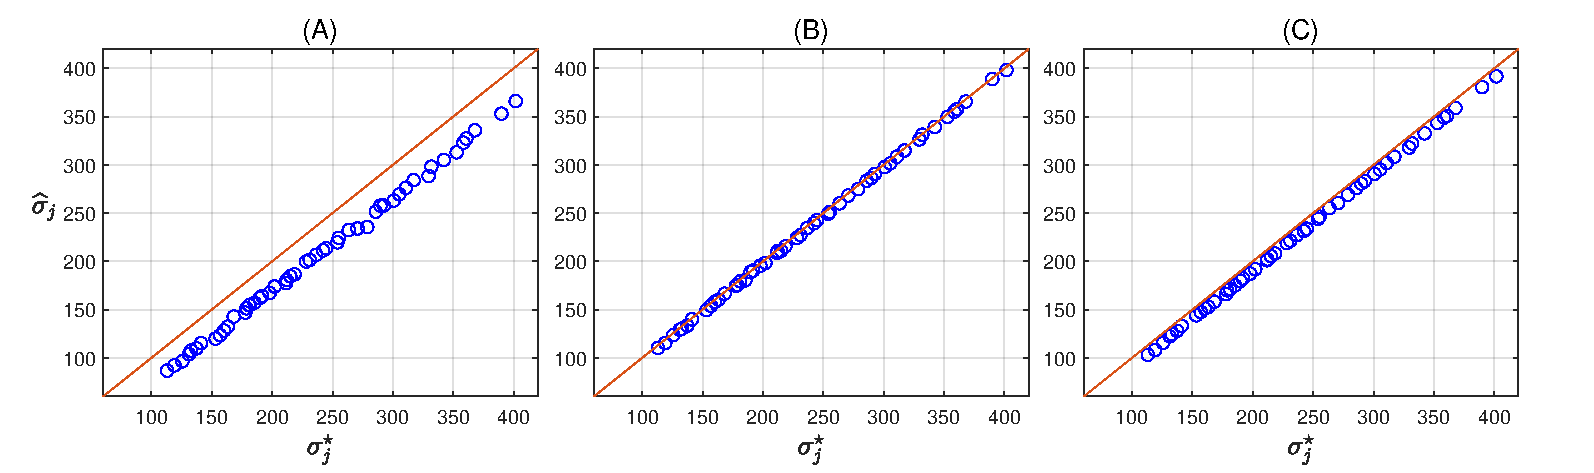
\includegraphics[width=150mm]{Figure/Fig1.pdf}
  \centering
  \caption{Three panels display the plots of estimated sigular values versus ground truth singular values $\sigma^{\star}_{j}$.
  The first two panels $(A)$ and $(B)$ are results from WMVR-ADMM algorithm with one weight update iteration under $n=250$.
  The panel $(C)$ exhibits the result when the estimator is obtained from SNN penalized least square under $n=1000$. }
  \label{Fig1}
\end{figure}

A following example demonstrates the sample efficiency of our proposed method for estimating the singular values of $\boldsymbol{\Theta^{\star}}$ when it is compared with the traditional SNN method.
We consider a setting of coefficient matrix $\boldsymbol{\Theta}^{\star}\in\mathbb{R}^{250 \times 250}$ with $r^{\star}=50$ and generate $\boldsymbol{A}, \boldsymbol{B} \in \mathbb{R}^{250 \times 50}$ with each entry from $\mathcal{N}(0,1)$ and set $\boldsymbol{\Theta}^{\star}=\boldsymbol{AB^{\top}}$.
Each entry of $\boldsymbol{X}\in\mathbb{R}^{n \times d_{1}}$ is sampled from $\mathcal{N}(0,1)$.
Variance parameter $\sigma$ is set as $1$, and hyper-tuning parameter $\boldsymbol{\lambda}_{n}$ is set as $5\sqrt{\frac{d_{1}+d_{2}}{n}}$, where $d_{1}=d_{2}=250$.
Panels in Figure~\ref{Fig1} display the plots of singular values of the minimizer $\widehat{\boldsymbol{\Theta}}$ in~\eqref{WMVR} against the singular values of ground-truth matrix $\boldsymbol{\Theta^{\star}}$.
Panel (A) exhibits the result of the first iteration of WMVR-ADMM with sample size $n=250$, and panel (B) exhibits the result of the second iteration of the algorithm with the updated weights.
Here, we set the $j^{\text{th}}$ weight $\omega_{j}$ as the inverse of the $j^{\text{th}}$ singular value of $\widehat{\boldsymbol{\Theta}}$ from the first iteration.
Note that we start the WMVR-ADMM with $\{\omega_{j}\}_{j=1}^{p}=1$, equivalent to solving SNN problem.
Panel (C) displays the result of SNN problem with $n=1000$.
It is worth noting that WMVR-ADMM achieves a satisfactory result within two iterations of loop with only $n=250$, whereas there is still a slight bias on each of the estimated singular value from SNN with $n=1000$.

\subsection{Additional Related Literature}
In the field of computer vision, many papers including \citet{gu2014weighted,gu2017weighted,xu2017multi,yair2018multi,liu2018speckle,kim2020cauchy} studied WNN minimization problem in the context of matrix completion problem.
However, from the statistical viewpoint, we are not aware of many works that apply the WNN in matrix regression problem except~\citet{chen2013reduced}.

In contrast, there are a myriad of papers which studied the statistical properties of SNN penalized least square problem under even a more general model than multivariate linear regression.
We only mention a subset of the long list.
\citet{bach2008consistency} provided necessary and sufficient conditions for the asymptotic rank consistency of SNN problem, and later~\citet{lee2015model} worked on proving the non-asymptotic rank consistency of the estimator from SNN under the irrepresentable assumption on design matrix.
Under the sub-Gaussian noise assumption,~\citet{negahban2011estimation} derived a minimax optimal rate of the estimation error of trace regression model when $\boldsymbol{\Theta}^{\star}$ is either approximately or exactly low rank matrix through the employment of the notion of restricted strong convexity (RSC) of the cost function.
Similarly, \citet{koltchinskii2011nuclear} established a sharp oracle inequality of the trace regression estimator under the restricted isometry condition of design matrix $\boldsymbol{X}$.
In the subsequent work,~\citet{fan2019generalized} investigated the SNN problem under generalized trace regression problems for categorical responses.
Recently, \citet{fan2021shrinkage} worked on obtaining the same minimax rate of trace regression problem with~\citet{negahban2011estimation} under the heavy-tail assumption on design matrix and observational noise.

Our work also falls into the category of adaptive penalized estimation problem.
Among a plethora of papers, we consider that the most relevant work with our paper is~\citet{zou2006adaptive}, which proposed the adaptive lasso in the context of sparse linear regression.
However, it is worth noting that once the weights are fixed, minimizing the least square fit with the adaptive $\ell_{1}$-penalization is always a convex optimization problem.
Later,~\citet{candes2008enhancing} suggested an algorithm for updating the weights in the adaptive lasso problem.
The main idea of their paper is to simply update the weights as the inverse of the estimated signal in the previous iteration.

\subsection{Organizations}
The rest of the paper is organized as follows.
In Section $2$, we introduce the details of WMVR-ADMM and provide a theorem on the algorithm's convergence guarantees.
In Section $3$, statistical properties of the estimator are provided.
First, in the orthogonal design setting, the non-asymptotic convergence rate of the singular values from the proposed estimator  $\{\sigma_{j}\big(\widehat{\boldsymbol{\Theta}}\big)\}_{j=1}^{p}$ is provided.
Second, under a Gaussian random design, we obtain the minimax rate of the estimation error.
In Section $4$, a two-stage data-driven method for updating weights and choosing the regularization parameter is detailed.
In Section $5$, we compare the performance of our estimator with SNN and an estimator from~\citet{chen2013reduced} in terms of estimation error under various model parameter settings.
In Section $6$, we apply our algorithm to a real data set to demonstrate the validity of WMVR-ADMM in practice.
Finally, we conclude our paper with the discussion section.

\section{WMVR-ADMM and Convergence Analysis}
In the first subsection, we describe the implementation of WMVR-ADMM algorithm for solving the non-convex optimization  problem~\eqref{WMVR}.
Then, in the next subsection, we present a convergence theorem of WMVR-ADMM algorithm.

\subsection{ADMM for Weighted Multivariate Regression} \label{WMVR-ADMM}
We start with reformulating~\eqref{WMVR} as follows:
\begin{align} \label{reform}
    \min_{\Theta, \boldsymbol{\Gamma}} \bigg\{ f(\boldsymbol{\Theta}) + g(\boldsymbol{\Gamma}) \bigg\}
    \qquad \textbf{s.t.} \qquad \boldsymbol{\Theta} = \boldsymbol{\Gamma} \in \mathbb{R}^{d_{1}\times d_{2}},
\end{align}
by letting $f(\boldsymbol{\Theta}):=\boldsymbol{\lambda}_{n}||\boldsymbol{\Theta}||_{\boldsymbol{\omega,\star}}$ and $g(\boldsymbol{\Gamma})=\frac{1}{2n}\|\boldsymbol{Y}-\boldsymbol{X}\boldsymbol{\Gamma}\|_{\text{F}}^{2}$.
This reformulation naturally leads to the construction of an augmented lagrangian function $\mathcal{L}_{\rho}\big(\boldsymbol{\Theta},\boldsymbol{\Gamma},\boldsymbol{\Lambda}\big)$ : For any $\rho>0$ and dual variable $\boldsymbol{\Lambda} \in \mathbb{R}^{d_{1}\times d_{2}}$, we define, 
\begin{align} \label{Lagrangian}
    \mathcal{L}_{\rho}\big(\boldsymbol{\Theta},\boldsymbol{\Gamma},\boldsymbol{\Lambda}\big):=
    f(\boldsymbol{\Theta}) + g(\boldsymbol{\Gamma}) + \textbf{tr}\big( \boldsymbol{\Lambda}^{\top}\big( \boldsymbol{\Theta}-\boldsymbol{\Gamma} \big)\big)
    + \frac{\rho}{2} || \boldsymbol{\Theta}-\boldsymbol{\Gamma} ||_{\text{F}}^{2}.
\end{align}
Then, we solve following three optimization problems repeatedly until primal and dual feasibility condition hold; that is, 
repeat \textbf{Steps 1-3},
\begin{align*}
    &\textbf{Step 1.} \quad \boldsymbol{\Theta}^{(k+1)} = \argmin_{\Theta \in \mathbb{R}^{d_{1} \times d_{2}}} \mathcal{L}_{\rho} \big( \boldsymbol{\Theta},\boldsymbol{\Gamma}^{(k)},\boldsymbol{\Lambda}^{(k)} \big), \\
    &\textbf{Step 2.} \quad \boldsymbol{\Gamma}^{(k+1)} = \argmin_{\boldsymbol{\Gamma} \in \mathbb{R}^{d_{1} \times d_{2}}} \mathcal{L}_{\rho} \big( \boldsymbol{\Theta}^{(k+1)},\boldsymbol{\Gamma},\boldsymbol{\Lambda}^{(k)} \big),  \\
    &\textbf{Step 3.} \quad \boldsymbol{\Lambda}^{(k+1)} = \boldsymbol{\Lambda}^{(k)} + \rho\big( \boldsymbol{\Theta}^{(k+1)}-\boldsymbol{\Gamma}^{(k+1)} \big),
\end{align*}
until $|| \boldsymbol{\Theta}^{(k+1)}-\boldsymbol{\Gamma}^{(k+1)} ||_{\text{F}}\leq 10^{-7}$ and $|| \boldsymbol{\Gamma}^{(k+1)}-\boldsymbol{\Gamma}^{(k)} ||_{\text{F}}\leq 10^{-7}$.
Here, we denote the tuple $(\boldsymbol{\Theta}^{(k)},\boldsymbol{\Gamma}^{(k)},\boldsymbol{\Lambda}^{(k)})$ as the updated parameters at $k^{\text{th}}$ iteration of the algorithm.
Note that the non-convexity of the landscape of the objective function in \textbf{Step 1} arises from the WNN  ( i.e., $\|\cdot\|_{\omega,\star}$) over $\boldsymbol{\Theta}$ with fixed $\boldsymbol{\Gamma}^{(k)},\boldsymbol{\Lambda}^{(k)}$, whereas the objective function in \textbf{Step 2} is a simple quadratic function of $\boldsymbol{\Gamma}$ with fixed $\boldsymbol{\Theta}^{(k+1)},\boldsymbol{\Lambda}^{(k)}$. 

We start the algorithm by initializing  $\boldsymbol{\Theta}^{(0)}=\boldsymbol{\Gamma}^{(0)}=\boldsymbol{\Lambda}^{(0)}=\boldsymbol{0} \in\mathbb{R}^{d_{1}\times d_{2}}$.
Next, the key of our algorithm is that a closed-form solution of \textbf{Step 1} can be obtained uniquely, even if it is a non-convex problem. 
We state the result in the following Lemma.
\begin{lemma} \label{Lemma2.1}
    Let $\boldsymbol{\Theta}^{(k+1)}$ be the minimizer of \textbf{Step 1}.
    Denote $\boldsymbol{B}^{(k)}:=-\boldsymbol{\Lambda}^{(k)}+\rho \cdot \boldsymbol{\Gamma}^{(k)}$ and its SVD as $\boldsymbol{U}^{\textbf{B}}\boldsymbol{D}^{\textbf{B}}\big(\boldsymbol{V}^{\textbf{B}}\big)^{\top}$.
    Then, for any fixed $\boldsymbol{\lambda}_{n}, \rho \geq 0 $ and $0\leq \omega_{1} \leq \dots \leq \omega_{p}$, 
    \begin{align*}
        &\boldsymbol{\Theta}^{(k+1)} = \boldsymbol{U}^{\textbf{B}}\mathcal{S}_{\boldsymbol{\lambda}_{n}\omega}\big(\boldsymbol{D}^{\textbf{B}}\big)\big(\boldsymbol{V}^{\textbf{B}}\big)^{\top}, \\ 
        &\mathcal{S}_{\boldsymbol{\lambda}_{n}\omega}\big(\boldsymbol{D}^{\textbf{B}}\big) = \text{diag}\bigg\{ \max\bigg\{\frac{1}{\rho}\big(\sigma_{j}(\boldsymbol{B}^{(k)}\big)-\boldsymbol{\lambda}_{n} w_{j}\big),0 \bigg\},  j=1,\dots,p \bigg\}.
    \end{align*}
    Furthermore, if all the non-zero singular values of $\boldsymbol{B}^{(k)}$ are distinct, then the solution $\boldsymbol{\Theta}^{(k+1)}$ is unique.
\end{lemma}

\begin{proof}
For simplicity, denote $\boldsymbol{B}^{(k)}:=-\boldsymbol{\Lambda}^{(k)}+\rho \cdot \boldsymbol{\Gamma}^{(k)}$, then we can solve the optimization problem in $\textbf{Step}\ \boldsymbol{1}$ as follows:
\begin{align}
    \boldsymbol{\Theta}^{(k+1)} 
    &= \argmin_{\boldsymbol{\Theta}\in\mathbb{R}^{d_{1} \times d_{2}}} \mathcal{L}_{\rho} \big( \boldsymbol{\Theta},\boldsymbol{\Gamma}^{(k)},\boldsymbol{\Lambda}^{(k)} \big) \nonumber \\
    &= \argmin_{\boldsymbol{\Theta}\in\mathbb{R}^{d_{1} \times d_{2}}}  \bigg\{ f(\boldsymbol{\Theta}) + \textbf{tr}\big(\boldsymbol{\Lambda}^{(k) \top}\boldsymbol{\Theta}\big) + \frac{\rho}{2} || \boldsymbol{\Theta}-\boldsymbol{\Gamma}^{(k)} ||_{\text{F}}^{2} \bigg\}  \nonumber \\
    &= \argmin_{\boldsymbol{\Theta}\in\mathbb{R}^{d_{1} \times d_{2}}} \bigg\{ \sum_{j=1}^{p} \bigg( \frac{\rho}{2}\sigma_{j}(\boldsymbol{\Theta})^{2} + \boldsymbol{\lambda}_{n} \omega_{j} \cdot\sigma_{j}(\boldsymbol{\Theta}) \bigg) -\textbf{tr} \big( \boldsymbol{B}^{(k) \top}\boldsymbol{\Theta} \big) \bigg\} \label{eq: step1_orig}.
\end{align}
We plugged-in $f(\boldsymbol{\Theta})=\boldsymbol{\lambda}_{n}||\boldsymbol{\Theta}||_{\boldsymbol{\omega,\star}}$, 
used $\textbf{tr}\big(\boldsymbol{\Theta}\boldsymbol{\Theta}^{\top}\big)=\sum_{j=1}^{p}\sigma_{j}\big(\boldsymbol{\Theta}\big)^{2}$ and the definition of $\boldsymbol{B}^{(k)}$ for deriving the last equality.
For further convenience of notation, let $\{d_{j}\}_{j=1}^{p}:=\{\sigma_{j}\big(\boldsymbol{\Theta}\big)\}_{j=1}^{p}$ and 
denote $\boldsymbol{\Theta}=\boldsymbol{UDV^{\top}}$ where 
$\boldsymbol{U}$ and $\boldsymbol{V}$ are the left and right singular matrices of $\boldsymbol{\Theta}$ and $\boldsymbol{D}:=\text{diag}\big(\{d_{1},d_{2},\dots,d_{p}\}\big)$.
Note that the entries in $\boldsymbol{D}$ are in non-increasing order. ( i.e. $d_{1} \geq d_{2} \dots \geq d_{p} \geq 0$)
Then, we can rewrite the optimization problem in~\eqref{eq: step1_orig} as follows:
\begin{align}
    \boldsymbol{\Theta}^{(k+1)} 
    &= \argmin_{d_{1}\geq d_{2}\geq \dots \geq d_{p} \geq 0 }\bigg\{ \sum_{j=1}^{p} \bigg( \frac{\rho}{2} d_{j}^{2} + \boldsymbol{\lambda}_{n}\omega_{j}d_{j} \bigg) - \max_{\boldsymbol{U}^{\top}\boldsymbol{U} = \mathcal{I}_{d_{1}}, \boldsymbol{V}^{\top}\boldsymbol{V} = \mathcal{I}_{d_{2}}} \textbf{tr}\big(\boldsymbol{B}^{(k)\top}\boldsymbol{\Theta}\big) \bigg\} \label{eq: step1_sec} 
\end{align}
The maximum of second term in~\eqref{eq: step1_sec} can be achieved when $\boldsymbol{U}$ and $\boldsymbol{V}$ coincide with 
left and right singular matrices of $\boldsymbol{B}^{(k)}$ respectively, giving us the maximized value as $\sum_{j=1}^{p}\sigma_{j}(\boldsymbol{B}^{(k)})d_{j}$.
This is a well-known Von Neumann's trace inequality.
See \cite{von1937some,mirsky1975trace}. 
Then, the final form of the optimization problem~\eqref{eq: step1_sec} reduces to obtaining the diagonal entries of the matrix $\boldsymbol{D}$ by minimizing a following : 
\begin{align}
    \min_{d_{1}\geq d_{2}\geq \dots \geq d_{p} \geq 0 }\bigg\{ \sum_{j=1}^{p} \bigg( \frac{\rho}{2} d_{j}^{2} + \big( \boldsymbol{\lambda}_{n} \omega_{j}-\sigma_{j}(\boldsymbol{B}^{(k)}) \big) d_{j} \bigg)  \bigg\}. \label{eq: step1}
\end{align}
The objective function~\eqref{eq: step1} is completely decompsable coordinate-wise and is minimized at $d_{j}=\max\big\{\frac{1}{\rho}\big(\sigma_{j}(\boldsymbol{B}^{(k)}\big)-\boldsymbol{\lambda}_{n} \omega_{j}\big),0 \big\}$ for $j=1,\dots,p$.
Since $\sigma_{1}(\boldsymbol{B}^{(k)})\geq\sigma_{2}(\boldsymbol{B}^{(k)})\dots\geq\sigma_{p}(\boldsymbol{B}^{(k)})$ and $0\leq\omega_{1}\leq\omega_{2}\leq\cdots\leq\omega_{p}$, the solution is feasible.
Furthermore, we have an unique minimizer due to the equality condition of von-Neumann's trace inequality when $\boldsymbol{B}^{(k)}$ has distinct non-zero singular values, and the uniqueness of strict convex optimization  of~\eqref{eq: step1} in $d_{j}$ for $j=1,\dots,p$. 
\qquad \qquad \qquad \qquad \qquad \qquad \qquad \qquad \qquad \qquad \qquad \qquad \qquad \qquad \qquad \qquad 
\qquad \qquad \qquad \qquad \qquad \qquad \quad \quad $\Box$
\end{proof}

Now, we turn our attention on minimizing the convex program in \textbf{Step 2}.
It is easy to rewrite and solve the problem in \textbf{Step 2} as follows: 
\begin{align}
    \boldsymbol{\Gamma}^{(k+1)} 
    &= \argmin_{\boldsymbol{\Gamma}\in\mathbb{R}^{d_{1} \times d_{2}}} \mathcal{L}_{\rho} \big( \boldsymbol{\Theta}^{(k+1)},\boldsymbol{\Gamma},\boldsymbol{\Lambda}^{(k)} \big) \nonumber \\
    &= \argmin_{\boldsymbol{\Gamma}\in\mathbb{R}^{d_{1} \times d_{2}}} \bigg\{ \textbf{tr} \bigg( \boldsymbol{\Gamma}^{\top}\bigg(\frac{1}{2n}\boldsymbol{X}^{\top}\boldsymbol{X} + \frac{\rho}{2} \cdot \mathcal{I}_{d_{1} \times d_{1}} \bigg) \boldsymbol{\Gamma} - \bigg( \frac{1}{n}\boldsymbol{Y}^{\top}\boldsymbol{X} + \rho \cdot \boldsymbol{\Theta}^{(k+1)} + \boldsymbol{\Lambda}^{(k)} \bigg)^{\top} \boldsymbol{\Gamma} \bigg) \bigg\} \label{eq: step2} \\ 
    &= \bigg( \frac{1}{n}\boldsymbol{X}^{\top}\boldsymbol{X}+\rho\cdot\mathcal{I}_{d_{1} \times d_{1}} \bigg)^{-1}\bigg( \frac{1}{n}\boldsymbol{Y}^{\top}\boldsymbol{X} +\rho \cdot \boldsymbol{\Theta}^{(k+1)} + \boldsymbol{\Lambda}^{(k)} \bigg). \label{eq: step2_sol} 
\end{align}
Note that the quadratic equation~\eqref{eq: step2} always has an unique minimizer~\eqref{eq: step2_sol} as long as $\rho>0$.
With the updated $\boldsymbol{\Theta}^{(k+1)}$ and $\boldsymbol{\Gamma}^{(k+1)}$ from $\textbf{Steps 1}, \textbf{2}$, we can easily update $\boldsymbol{\Lambda}^{(k)}$ to $\boldsymbol{\Lambda}^{(k+1)}$ through $\textbf{Step 3}$.
The final output of WMVR-ADMM is a minimizer of $\mathcal{L}_{\rho} \big( \boldsymbol{\Theta},\boldsymbol{\Gamma}^{(\mathcal{T}-1)},\boldsymbol{\Lambda}^{(\mathcal{T}-1)}\big)$ in $\textbf{Step 1}$, where $\mathcal{T}$ denotes the last iteration index of the algorithm.
Therefore, as long as all the non-zero singular values of $\boldsymbol{B}^{(\mathcal{T})}$ are distinct, then the WMVR-ADMM has an unique solution.
The entire implementation of WMVR-ADMM is summarized in Algorithm~\ref{alg:1}.

\begin{algorithm}[t] 
    \textbf{Input} : A measurement pair $\big( \boldsymbol{X}, \boldsymbol{Y} \big)$, $\boldsymbol{\lambda}_{n} \geq 0$ and $0\leq \omega_{1} \leq \dots \leq \omega_{p}$. \\
    \textbf{Initialization} : $\boldsymbol{\Theta}^{(0)}=\boldsymbol{\Gamma}^{(0)}=\boldsymbol{\Lambda}^{(0)}=\boldsymbol{0} \in\mathbb{R}^{d_{1}\times d_{2}}$. \\
    {\bf Repeat following Steps :} \\
    \qquad {\bf Step 1.} Let $\boldsymbol{B^{(k)}}:=-\boldsymbol{\Lambda}^{(k)}+\rho \cdot \boldsymbol{\Gamma}^{(k)}$.
    \quad $\boldsymbol{B^{(k)}}=\boldsymbol{U}^{\textbf{B}}\boldsymbol{D}^{\textbf{B}}\big(\boldsymbol{V}^{\textbf{B}}\big)^{\top}$. \\
    \qquad \qquad \qquad Set $\mathcal{S}_{\boldsymbol{\lambda}_{n}\omega}\big(\boldsymbol{D}^{\textbf{B}}\big)=\textbf{diag}\bigg\{ \max\bigg\{\frac{1}{\rho}\big(\sigma_{j}(\boldsymbol{B}^{(k)}\big)-\boldsymbol{\lambda}_{n} w_{j}\big),0 \bigg\}$ for $j=1,\dots,p \bigg\}$.  \\
    \qquad \qquad \qquad $\boldsymbol{\Theta}^{(k+1)} = \boldsymbol{U}^{\textbf{B}}\mathcal{S}_{\boldsymbol{\lambda}_{n}\omega}\big(\boldsymbol{D}^{\textbf{B}}\big)\big(\boldsymbol{V}^{\textbf{B}}\big)^{\top}$ \\
    \qquad {\bf Step 2.} 
    $\boldsymbol{\Gamma}^{(k+1)} = \big( \frac{1}{n}\boldsymbol{X}^{\top}\boldsymbol{X}+\rho\cdot\mathcal{I}_{d_{1} \times d_{1}} \big)^{-1}\big( \frac{1}{n}\boldsymbol{Y}^{\top}\boldsymbol{X} + \rho \cdot \boldsymbol{\Theta}^{(k+1)} + \boldsymbol{\Lambda}^{(k)} \big).$\\
    \qquad {\bf Step 3.} $\boldsymbol{\Lambda}^{(k+1)} = \boldsymbol{\Lambda}^{(k)} + \rho\big( \boldsymbol{\Theta}^{(k+1)}-\boldsymbol{\Gamma}^{(k+1)} \big)$.\\
    {\bf Until} $|| \boldsymbol{\Theta}^{(k+1)}-\boldsymbol{\Gamma}^{(k+1)} ||_{\text{F}}\leq 10^{-7}$ and $|| \boldsymbol{\Gamma}^{(k+1)}-\boldsymbol{\Gamma}^{(k)} ||_{\text{F}}\leq 10^{-7}$. \\
    \textbf{Output} : $\widehat{\boldsymbol{\Theta}}=\boldsymbol{\Theta}^{(k+1)}$. 
    \caption{ADMM for Weighted Multi-Variate Regression. (WMVR-ADMM)}
    \label{alg:1}
\end{algorithm}

\begin{remark}
We want to note that WMVR-ADMM algorithm can be easily extended to trace regression model, which is a general model of multivariate linear regression model.\footnote{Refer~\citet{negahban2011estimation} for checking how to translate MVLR to trace regression model.}
In order for the concise presentation of the paper, we defer the detailed descriptions of the extended algorithm to trace regression model in the Appendix~\ref{tr_algo}.
\end{remark}

\subsection{Convergence of WMVR-ADMM}
In this subsection, the Theorem~\ref{convergence} on the convergence of WMVR-ADMM is presented with some remarks.
Then, two lemmas for proof of the theorems are provided.
Finally, we conclude the subsection with the proof of Theorem~\ref{convergence}.

\begin{theorem} \label{convergence}
    Set $\rho>2L_{\nabla g}$ with $L_{\nabla g}:=\sigma_{1}\big( \frac{1}{n}\boldsymbol{X}^{\top}\boldsymbol{X}\big)$.
    The sequence $\{(\boldsymbol{\Theta}^{(k)},\boldsymbol{\Gamma}^{(k)},\boldsymbol{\Lambda}^{(k)})\}_{k \geq 1}$ from WMVR-ADMM converges globally to the unique stationary point of $\mathcal{L}_{\rho}(\boldsymbol{\Theta},\boldsymbol{\Gamma},\boldsymbol{\Lambda})$.
\end{theorem}

The threshold for penalty parameter $\rho$ can be computed from data.
Here, ``globally'' means regardless of where the initial point under non-convex landscape of~\eqref{Lagrangian}.
This is verified numerically in subsection~\ref{conv_exp}.
The uniqueness claim is due from the fact that the augmented lagrangian function~\eqref{Lagrangian} is a Kurdyka-Lojasiewicz (KL) function.
This is further elaborated in sub-subsection~\ref{proof_conv} with relevant references.
The proof of Theorem~\ref{convergence} is motivated from~\citet{wang2019global} and~\citet{kim2020cauchy}.
The key two ingredients are provided as follows.
The detailed proofs of following two Lemmas are in the Appendix. 
\begin{lemma} \label{Lemma2.3}
Set $\rho>2L_{\nabla g}$ with $L_{\nabla g}:=\sigma_{1}\big( \frac{1}{n}\boldsymbol{X}^{\top}\boldsymbol{X}\big)$.
Then, the iterates $\{(\boldsymbol{\Theta}^{(k)},\boldsymbol{\Gamma}^{(k)},\boldsymbol{\Lambda}^{(k)})\}_{k \geq 1}$ generated from WMVR-ADMM satisfy followings : 
\begin{enumerate}
    \item $\mathcal{L}_{\rho} \big( \boldsymbol{\Theta}^{(k)},\boldsymbol{\Gamma}^{(k)},\boldsymbol{\Lambda}^{(k)} \big)$ is lower-bounded and non-increasing over $k \geq 1$.
    \item $\{(\boldsymbol{\Theta}^{(k)},\boldsymbol{\Gamma}^{(k)},\boldsymbol{\Lambda}^{(k)})\}_{k \geq 1}$ is bounded.
    \item $\left\| \boldsymbol{\Theta}^{(k)} - \boldsymbol{\Gamma}^{(k)} \right\|_{\text{F}}\rightarrow{0}$ \quad and 
    \quad $\left\| \boldsymbol{\Gamma}^{(k+1)} - \boldsymbol{\Gamma}^{(k)} \right\|_{\text{F}}\rightarrow{0}$, \quad as
    $k\rightarrow{\infty}$.
\end{enumerate}
\end{lemma}

\begin{lemma} \label{Lemma2.4}
For $k\geq 1$, there exist a constant $C_{2}>0$ and $p^{(k+1)}\in\partial \mathcal{L}_{\rho} \big( \boldsymbol{\Theta}^{(k+1)},\boldsymbol{\Gamma}^{(k+1)},\boldsymbol{\Lambda}^{(k+1)} \big)$ such that $\|p^{(k+1)}\|_{\text{F}}\leq C_{2} \| \boldsymbol{\Gamma}^{(k+1)} - \boldsymbol{\Gamma}^{(k)} \|_{\text{F}}$.
\end{lemma}

\subsubsection{Proof of Theorem 2} \label{proof_conv}
The proof of Theorem~\ref{convergence} is divided into five steps. 
We provide each steps sequentially.\\ \\
{\textbf{Step 1.}}
By Bolzano-Weierstrass threorem, we know the bounded sequence $\{\boldsymbol{\Theta}^{(k)},\boldsymbol{\Gamma}^{(k)},\boldsymbol{\Lambda}^{(k)}\}_{k \geq 0}$ has a convergent subsequence
$\{\boldsymbol{\Theta}^{(k_{s})},\boldsymbol{\Gamma}^{(k_{s})},\boldsymbol{\Lambda}^{(k_{s})}\}_{s \geq 1}$, and denote its limit point as $(\boldsymbol{\Theta}^{*},\boldsymbol{\Gamma}^{*},\boldsymbol{\Lambda}^{*})$. 
\\ \\
{\textbf{Step 2.}}
Since the augmented lagrangian function $\mathcal{L}_{\rho} \big( \boldsymbol{\Theta}^{(k)},\boldsymbol{\Gamma}^{(k)},\boldsymbol{\Lambda}^{(k)} \big)$ is non-increasing and bounded from below,
the sequence $\{\mathcal{L}_{\rho} \big( \boldsymbol{\Theta}^{(k)},\boldsymbol{\Gamma}^{(k)},\boldsymbol{\Lambda}^{(k)} \big)\}_{k \geq 0}$ converges.
\\ \\
{\textbf{Step 3.}}
By continuity of $\mathcal{L}_{\rho} \big( \boldsymbol{\Theta}^{(k)},\boldsymbol{\Gamma}^{(k)},\boldsymbol{\Lambda}^{(k)} \big)$ and results from \textbf{Step 1} and \textbf{Step 2}, we have
\begin{align*}
    \lim_{k\rightarrow{\infty}} \mathcal{L}_{\rho} \big( \boldsymbol{\Theta}^{(k)},\boldsymbol{\Gamma}^{(k)},\boldsymbol{\Lambda}^{(k)} \big)
    = \lim_{s\rightarrow{\infty}} \mathcal{L}_{\rho} \big( \boldsymbol{\Theta}^{(k_{s})},\boldsymbol{\Gamma}^{(k_{s})},\boldsymbol{\Lambda}^{(k_{s})} \big)
    = \mathcal{L}_{\rho} \big( \boldsymbol{\Theta}^{*},\boldsymbol{\Gamma}^{*},\boldsymbol{\Lambda}^{*} \big).
\end{align*}
\noindent {\textbf{Step 4.}}
By the result of Lemma $2.4$, there exists $p^{(k+1)}\in\partial \mathcal{L}_{\rho} \big( \boldsymbol{\Theta}^{(k+1)},\boldsymbol{\Gamma}^{(k+1)},\boldsymbol{\Lambda}^{(k+1)} \big)$ such that $\left\|p^{(k+1)}\right\|_{\text{F}}\rightarrow{0}$ as $k\rightarrow{\infty}$.
Consequently, we conclude the following:
\begin{align*}
    p^{(k+1)}\in\partial \mathcal{L}_{\rho} \big( \boldsymbol{\Theta}^{(k+1)},\boldsymbol{\Gamma}^{(k+1)},\boldsymbol{\Lambda}^{(k+1)} \big) \rightarrow{ \boldsymbol{0}\in\partial \mathcal{L}_{\rho} \big( \boldsymbol{\Theta}^{*},\boldsymbol{\Gamma}^{*},\boldsymbol{\Lambda}^{*} \big)}, \quad
    k\rightarrow{\infty}.
\end{align*}
\noindent {\textbf{Step 5.}}
It remains to prove $\mathcal{L}_{\rho}$ is a Kurdyka-Lojasiewicz (KL) function for ensuring the generated sequence
$\{(\boldsymbol{\Theta}^{(k)},\boldsymbol{\Gamma}^{(k)}$,\\
$\boldsymbol{\Lambda}^{(k)})\}_{k \geq 0}$ converges globally to the unique point 
$\{\boldsymbol{\Theta}^{*},\boldsymbol{\Gamma}^{*},\boldsymbol{\Lambda}^{*}\}$.
See Proposition $2$ in~\citet{wang2019global} and Theorem $2.9$ in~\citet{attouch2013convergence}.
If a function is semi-algebraic, then it is known to be a KL function~\citep{attouch2013convergence,sun2017global}.
Refer~\citet{sun2017global} for the definition of semi-algebraic function.
Since $\frac{1}{2n}\left\| \boldsymbol{Y}-\boldsymbol{X\Gamma} \right\|_{\text{F}}^{2}+\textbf{tr}\big( \boldsymbol{\Lambda}^{\top}\big( \boldsymbol{\Theta}-\boldsymbol{\Gamma} \big)\big)$ is a real-polynomial function, it is semi-algebraic.
Since the finite sum of semi-algebraic functions are semi-algebraic~\citep{attouch2013convergence}, it remains to prove $\lambda_{n}\|\boldsymbol{\Theta}\|_{\omega,*}$ is a semi-algebraic. 
In proposition $3$ of~\citet{sun2017global}, it is proved that each singular value of the matrix $\boldsymbol{\Theta}$, $\sigma_{j}(\boldsymbol{\Theta})$, is a semi-algebraic.
Therefore, the weighted singular value $\omega_{j}\sigma_{j}(\boldsymbol{\Theta})$ is also a semi-algebraic function, and finally, summing rule gives that $\lambda_{n}\|\boldsymbol{\Theta}\|_{\omega,*}$ is a semi-algebraic function. 
\qquad \qquad $\Box$

\section{Statistical Properties of the Estimator}
In this section, we explore statistical properties of the proposed estimator.
In subsection $3.1$, the non-asymptotic property of the proposed estimator under orthogonal design setting is studied, which sheds lights on understanding the role of weights on the estimation of singular values. 
In subsection $3.2$, the minimax convergence rate of the estimation error is derived under a Gaussian design setting.

\subsection{Statistical Properties of $\widehat{\boldsymbol{\Theta}}$ under Orthogonal Design}
We first study the convergent rate of estimated eigenvalues $\sigma_{j}\big(\widehat{\boldsymbol{\Theta}}\big)$ for $j = 1, \cdots, p$.
The result with its proof is provided below.

\begin{proposition} \label{clsed-form}
    Suppose .
    Let $\widehat{\boldsymbol{U}}^{\text{LS}}\widehat{\boldsymbol{D}}^{\text{LS}}\big(\widehat{\boldsymbol{V}}^{\text{LS}}\big)^{\top}$ be SVD of the least-square estimator $\widehat{\boldsymbol{\Theta}}^{\text{LS}}:=\big(\boldsymbol{X}^{\top}\boldsymbol{X}\big)^{-1}\boldsymbol{X}^{\top}\boldsymbol{Y}$.
    Then, under the orthogonal design (i.e., $\boldsymbol{X}^{\top}\boldsymbol{X}=n\boldsymbol{I}_{d_{1} \times d_{1}}$), SVD of the minimizer of~\eqref{WMVR} has a following closed-form solution:
    $\widehat{\boldsymbol{\Theta}} := \widehat{\boldsymbol{U}}^{\text{LS}}\widehat{\boldsymbol{D}}\big(\widehat{\boldsymbol{V}}^{\text{LS}}\big)^{\top}$,
    where the diagonal entry of $\widehat{\boldsymbol{D}}$ is:
    $\sigma_{j}\big(\widehat{\boldsymbol{\Theta}}\big) = \max \big(  \sigma_{j}\big(\widehat{\boldsymbol{\Theta}}^{\text{LS}}\big)-\boldsymbol{\lambda}_{n} \omega_{j},0 \big)$ for $j=1,\dots,p$.
    Furthermore, suppose $\boldsymbol{\lambda}_{n}=\sqrt{\frac{d_{1}+d_{2}}{n}}$.
    Then, with probability at least $1-2\exp(-(\sqrt{d_{1}}+\sqrt{d_{2}})^{2}/2)$, we have,
    \begin{align} \label{sing1}
        \left| \sigma_{j}\big(\widehat{\boldsymbol{\Theta}}\big)-\sigma_{j}\big(\boldsymbol{\Theta}^{\star}\big)\right|
        &\leq \max\big(4\sigma,2\omega_{j}\big)\cdot \sqrt{\frac{d_{1}+d_{2}}{n}},
    \end{align}
    for $j$ such that $\sigma_{j}\big(\boldsymbol{\Theta}^{\star}\big)>0$.
    With the same probability bound, we have,
    \begin{align} \label{sing2}
        \left| \sigma_{j}\big(\widehat{\boldsymbol{\Theta}}\big)\right|
        &\leq \min\big(2\sigma,\omega_{j}\big)\cdot \sqrt{\frac{d_{1}+d_{2}}{n}},
    \end{align}
    for $j$ such that $\sigma_{j}\big(\boldsymbol{\Theta}^{\star}\big)=0$.
\end{proposition}
\begin{proof}
The derivation on the closed-form solution of $\widehat{\boldsymbol{\Theta}}$ is exactly same with that of Lemma $1$ in~\citet{yuan2007dimension}, under the orthogonal design assumption.
So we omit the proof.
We only focus on controlling the distance between singular values of $\widehat{\boldsymbol{\Theta}}$ and $\boldsymbol{\Theta}^{\star}$.
With the equality $\boldsymbol{Y}=\boldsymbol{X}\boldsymbol{\Theta}^{\star}+\boldsymbol{E}$ and $\boldsymbol{X}^{\top}\boldsymbol{X}=n\boldsymbol{I}_{d_{1} \times d_{1}}$, we have
\begin{align} \label{OLS}
    \widehat{\boldsymbol{\Theta}}^{\text{LS}}=\big(\boldsymbol{X}^{\top}\boldsymbol{X}\big)^{-1}\boldsymbol{X}^{\top}\boldsymbol{Y} = \boldsymbol{\Theta^\star} + \frac{\boldsymbol{X}^{\top}\boldsymbol{E}}{n}.
\end{align}
By the corollary of Weyl's Theorem and the equality~\eqref{OLS}, inequality
\begin{align} \label{sing_ineq}
    \max_{j=1,\dots,p}\left| \sigma_{j}\big(\widehat{\boldsymbol{\Theta}}^{\text{LS}}\big) - \sigma_{j}\big(\boldsymbol{\Theta^\star}\big) \right|
    \leq \sigma_{1}\bigg( \frac{\boldsymbol{X}^{\top}\boldsymbol{E}}{n} \bigg).
\end{align}
can be obtained. Recall from our problem setting that the rows of $\boldsymbol{E}$ are independent from $\mathcal{N}(0,\sigma^{2}\boldsymbol{I}_{d_{2} \times d_{2}})$.
Therefore, we know each entry of $\boldsymbol{X}^{\top}\boldsymbol{E}/\sigma\sqrt{n}$ follows $\mathcal{N}(0,1)$ and is independent with each other.
Following Chapter $6$ in~\cite{wainwright2019high},
with probability at least $1-2\exp(-(\sqrt{d_{1}}+\sqrt{d_{2}})^{2}/2)$, the right hand side of (\ref{sing_ineq}) satisfies
\begin{align} \label{Singular_bnd}
    \sigma_{1}\bigg( \frac{\boldsymbol{X}^{\top}\boldsymbol{E}}{n} \bigg) \leq 2\sigma \sqrt{\frac{d_{1}+d_{2}}{n}} .
\end{align}
Because $\sigma_{j}\big(\widehat{\boldsymbol{\Theta}}\big) = \sigma_{j}\big(\widehat{\boldsymbol{\Theta}}^{\text{LS}}\big)-\boldsymbol{\lambda}_{n} w_{j}>0$ for $j=1,\dots,\widehat{r}$, with further combing (\ref{sing_ineq}) and (\ref{Singular_bnd}), we know  for $j\in\{1,\dots,\widehat{r}\}$
\begin{align}
    \left| \sigma_{j}\big(\widehat{\boldsymbol{\Theta}}\big)-\sigma_{j}\big(\boldsymbol{\Theta}^{\star}\big)\right|
    &= \left|\sigma_{j}\big(\widehat{\boldsymbol{\Theta}}^{\text{LS}}\big)-\boldsymbol{\lambda}_{n}\omega_{j}
    -\sigma_{j}\big(\boldsymbol{\Theta}^{\star}\big)\right| \nonumber \\
    &\leq \left|\sigma_{j}\big(\widehat{\boldsymbol{\Theta}}^{\text{LS}}\big)
    -\sigma_{j}\big(\boldsymbol{\Theta}^{\star}\big)\right| + \boldsymbol{\lambda}_{n}\omega_{j} \nonumber \\
    &\leq \sigma_{1}\bigg( \frac{\boldsymbol{X}^{\top}\boldsymbol{E}}{n} \bigg) + \boldsymbol{\lambda}_{n}\omega_{j}
    \leq \max\big(4\sigma,2\omega_{j}\big)\cdot \sqrt{\frac{d_{1}+d_{2}}{n}},  \nonumber
\end{align}
where in the last inequality, we use~\eqref{Singular_bnd} and choose $\boldsymbol{\lambda}_{n}=\sqrt{\frac{d_{1}+d_{2}}{n}}$. For $j\in\{\widehat{r}+1,\dots,p\}$ such that $\sigma_{j}\big( \boldsymbol{\Theta}^{\star} \big) > 0$, the following inequalities hold
\begin{align}
    \left| \sigma_{j}\big(\widehat{\boldsymbol{\Theta}}\big)-\sigma_{j}\big(\boldsymbol{\Theta}^{\star}\big)\right|
    &\leq \left|\sigma_{j}\big(\widehat{\boldsymbol{\Theta}}^{\text{LS}}\big)
    -\sigma_{j}\big(\boldsymbol{\Theta}^{\star}\big)\right| + \left| \sigma_{j}\big(\widehat{\boldsymbol{\Theta}}^{\text{LS}}\big) \right| \nonumber \\
    &\leq \sigma_{1}\bigg( \frac{\boldsymbol{X}^{\top}\boldsymbol{E}}{n} \bigg) + \boldsymbol{\lambda}_{n}\omega_{j}
    \leq \max\big(4\sigma,2\omega_{j}\big)\cdot \sqrt{\frac{d_{1}+d_{2}}{n}},  \nonumber
\end{align}
where in the second inequality, we use~\eqref{sing_ineq} and $| \sigma_{j}\big(\widehat{\boldsymbol{\Theta}}^{\text{LS}}\big) |\leq \boldsymbol{\lambda}_{n}\omega_{j}$ for $j\in\{\widehat{r}+1,\dots,p\}$.
For $j \in \{\widehat{r}+1,\dots,p\}$ such that $\sigma_{j}\big( \boldsymbol{\Theta}^{\star} \big) = 0$, we have the following result:
\begin{align}\label{thrd_case}
    \left| \sigma_{j}\big(\widehat{\boldsymbol{\Theta}}\big)-\sigma_{j}\big(\boldsymbol{\Theta}^{\star}\big)\right|
    &\leq \left| \sigma_{j}\big(\widehat{\boldsymbol{\Theta}}^{\text{LS}}\big) \right| \leq \boldsymbol{\lambda}_{n}\omega_{j}.
\end{align}
Using that the three inequalities~\eqref{sing_ineq},~\eqref{Singular_bnd}, and~\eqref{thrd_case} should hold at the same time, we can conclude the proof.
\qquad $\Box$
\end{proof}

Based on the closed-form solution of $\widehat{\boldsymbol{\Theta}}$ in Proposition~\ref{clsed-form}, under the orthogonal design assumption, each estimated singular value has a form $\max \big( \sigma_{j}\big(\widehat{\boldsymbol{\Theta}}^{\text{LS}}\big)-\boldsymbol{\lambda}_{n} \omega_{j},0 \big)$ for $j\in\{1,\dots,p\}$.
Then, for the fixed $\boldsymbol{\lambda}_{n}$, it is easy to see that the large weights for small singular values of $\widehat{\boldsymbol{\Theta}}^{\text{LS}}$ can induce the sparsity among the singular values of $\widehat{\boldsymbol{\Theta}}$.
Furthermore, the proposition states that with an appropriate choice of tuning parameter $\boldsymbol{\lambda}_{n}$, the singular values of the $\widehat{\boldsymbol{\Theta}}$ are consistently estimated.
Bounds in~\eqref{sing1} and~\eqref{sing2} provide us with the guideline for the choices of weights.
That is, for the set of indices of $\sigma_{j}\big(\boldsymbol{\Theta}^{\star}\big)>0$, the corresponding weights $\omega_{j}$s need to be set lower than the twice of variance size of the measurement error $\sigma$, whereas, for the set of indices whose $\sigma_{j}\big(\boldsymbol{\Theta}^{\star}\big)=0$, the corresponding weights can be set even higher than $2\sigma$.
This is consistent with our intuition that we need small weights for estimating non-zero singular values of $\boldsymbol{\Theta}^{\star}$, whereas large weights are required for the consistent estimation of zero singular values of $\boldsymbol{\Theta}^{\star}$.

\subsection{Estimation Error under Random Design}
We further study the estimation error in Frobenius norm (i.e., $\| \widehat{\boldsymbol{\Theta}} - \boldsymbol{\Theta^{\star}} \|_{\text{F}}^{2}$)  under a random design assumption.
Specifically, we begin this subsection by providing the additional assumptions on model, which will be used for stating our theorem.
Then, with a brief introduction of the framework on which our theorem is based, an important Lemma on the subset $\mathcal{C}$, where the error matrix $\widehat{\boldsymbol{\Theta}}-\boldsymbol{\Theta^{\star}}$ belongs, is provided.
Finally, we state our main Theorem.

\subsubsection{Additional Assumptions}
A design matrix $\boldsymbol{X}$ is assumed to be random, whose rows are independently sampled from $d_{1}$-variate $\mathcal{N}(0,\boldsymbol{\Sigma})$ distribution for some positive definite covariance matrix $\boldsymbol{\Sigma}\in\mathbb{R}^{d_{1} \times d_{1}}$.
Additionally, we relax the assumption of $\boldsymbol{\Theta}^{\star}$ from a exact low rank setting to a nearly low-rank matrix by requiring that the $\{\sigma_{j}\big(\boldsymbol{\Theta}^{\star}\big)\}_{j=1}^{p}$ decays fast enough.
Specifically, for a parameter $q\in[0,1]$ and a radius $r^{\star}$, we assume that
\begin{align*}
    \boldsymbol{\Theta}^{\star} \in \mathbb{B}_{q}(r^{\star})
    := \bigg\{ \boldsymbol{\Theta}\in\mathbb{R}^{d_{1} \times d_{2}} :
    \sum_{j=1}^{p} \left| \sigma_{j}\big(\boldsymbol{\Theta}^{\star} \big) \right|^{q} \leq r^{\star}
    \bigg\}.
\end{align*}
Note that when $q=0$, the set $\mathbb{B}_{q}(r^{\star})$ becomes the set of matrices with rank at most $r^{\star}$.
Additionally, we assume that $\boldsymbol{\widehat{\Theta}}$ is a global minimizer of~\eqref{WMVR}.

\subsubsection{General Framework and Characterization of Subset $\mathcal{C}$} \label{GF}
There are two key ingredients that will be used for studying the estimation errors : $(\RN{1})$ restricted strong convexity of the cost function $\mathcal{L}_{n}(\boldsymbol{\Theta}):= \frac{1}{2n} \left\| \boldsymbol{Y}-\boldsymbol{X}\boldsymbol{\Theta} \right\|_{\text{F}}^{2}$ around $\Theta^\star$ and
$(\RN{2})$ the characterization of set where the associated error matrix $\boldsymbol{\widehat{\Delta}}=\widehat{\boldsymbol{\Theta}}-\boldsymbol{\Theta^{\star}}$ belongs.
In high-dimensional setting where $n \ll d_{1}d_{2}$, although the function $\mathcal{L}_{n}(\boldsymbol{\Theta})$ might be curved in some directions, there are $\big(d_{1}d_{2}-n\big)$ directions where it is flat up to second order.
We hope that the associated error matrix $\boldsymbol{\widehat{\Delta}}$
lies in some directions $\mathcal{C}\subseteq \mathbb{R}^{d_{1}\times d_{2}}$ where the $\mathcal{L}_{n}(\boldsymbol{\Theta})$ is curved.
This notion is neatly expressed as follows: for some positive constant $\kappa>0$,
\begin{align} \label{RSC}
    \mathcal{E}_{n}\big(\boldsymbol{\widehat{\Delta}})\geq \kappa || \boldsymbol{\widehat{\Delta}} ||_{\text{F}}^{2} \qquad \text{for all} \quad \boldsymbol{\widehat{\Delta}}\in\mathcal{C},
\end{align}
where $\mathcal{E}_{n}\big(\boldsymbol{\widehat{\Delta}})$ denotes the first order Taylor-expansion error of $\mathcal{L}_{n}(\cdot)$ around $\boldsymbol{\Theta}^\star$.
In other words, we call $\mathcal{E}_{n}\big(\boldsymbol{\widehat{\Delta}})$ succeeds \textit{``restricted strong convexity''} (RSC) over the set $\mathcal{C}$ if there exists $\kappa>0$.
Fortunately, under multivariate regression model with Gaussian ensemble, we can prove that the RSC condition indeed holds with $\kappa=\frac{\sigma_{\text{min}}(\boldsymbol{\Sigma})}{18}$ in high probability over $\mathbb{R}^{d_{1} \times d_{2}}$,
\footnote{See Lemma $2$ in~\citet{negahban2011estimation} and Appendix~\ref{pf_thm_3_2} of our paper for the proof on this fact.} where $\sigma_{\text{min}}(\boldsymbol{\Sigma})$ denotes a minimum eigenvalue of $\boldsymbol{\Sigma}$.

Before we formally state the Lemma which characterizes the set $\mathcal{C}$, let us introduce relevant notations.
Denote $\boldsymbol{U}^{\star}$ and $\boldsymbol{V}^{\star}$ as the left and right singular matrices of $\boldsymbol{\Theta}^{\star}$.
The $\mathcal{M}_{r}\big( \mathcal{U}, \mathcal{V} \big)$ ( resp. $\overline{\mathcal{M}}_{r}^{\perp}\big( \mathcal{U}, \mathcal{V} \big)$ ) corresponds to subspace of matrices with non-zero left and right singular vectors associated with the first $r$ ( resp.  remaining $(p-r)$ ) columns of $\boldsymbol{U}^{\star}$ and $\boldsymbol{V}^{\star}$.
That is, for any given integer $r\leq p$, we have
\begin{align*}
    &\mathcal{M}_{r}\big( \mathcal{U}, \mathcal{V} \big) = \big\{ \boldsymbol{\Theta}\in\mathbb{R}^{d_{1} \times d_{2}} : \textbf{colspan}(\boldsymbol{\Theta}) \subseteq \mathcal{U},\quad  \textbf{rowspan}(\boldsymbol{\Theta}) \subseteq \mathcal{V}  \big\} \\
    &\overline{\mathcal{M}}_{r}^{\perp}\big( \mathcal{U}, \mathcal{V} \big) = \big\{ \boldsymbol{\Theta}\in\mathbb{R}^{d_{1} \times d_{2}} : \textbf{colspan}(\boldsymbol{\Theta}) \subseteq \mathcal{U}^{\perp},\quad  \textbf{rowspan}(\boldsymbol{\Theta}) \subseteq \mathcal{V}^{\perp} \big\}.
\end{align*}
Then, $\mathcal{U}$ and $\mathcal{V}$ are the r-dimensional subspaces of vectors from the first r columns of matrices $\boldsymbol{U}^{\star}$ and $\boldsymbol{V}^{\star}$.
Moreover, $\mathcal{U}^{\perp}$ and $\mathcal{V}^{\perp}$ denote the subspaces orthogonal to  $\mathcal{U}$ and $\mathcal{V},$ respectively, and $\textbf{colspan}(\boldsymbol{\Theta})$ and $\textbf{rowspan}(\boldsymbol{\Theta})$ denote the column space and row space of $\boldsymbol{\Theta}$.
Hereafter, we will omit $\mathcal{U}$ and $\mathcal{V}$ from the notations, if they are clear from the context.

\begin{lemma} \label{Cone_like_set}
Suppose $\widehat{\boldsymbol{\Theta}}$ is an global minimizer of the~\eqref{WMVR} obtained from WMVR-ADMM, with the associated matrix $\boldsymbol{\widehat{\Delta}} = \widehat{\boldsymbol{\Theta}}-\boldsymbol{\Theta^{\star}}$.
Set the weights $\frac{1}{2} < \omega_{1} \leq \dots \leq \omega_{p}$ and
suppose regularization parameter is chosen such that $\boldsymbol{\lambda}_{n}\geq\frac{2}{n}\left\| \boldsymbol{X}^{\top}\boldsymbol{E} \right\|_{\text{op}}$.
Let $\|\cdot\|_{\star}:=\sum_{j=1}^{p}\sigma_{j}(\cdot)$.
Then, for a positive integer $r\leq p$, we have
\begin{align} \label{cone_set}
    \mathcal{C}\big( \omega;r;\delta \big)
    := \bigg\{ \boldsymbol{\widehat{\Delta}}\in\mathbb{R}^{d_{1}\times d_{2}} :
    ||\boldsymbol{\widehat{\Delta}}''||_{\star} \leq \frac{2w_{p}}{w_{1}-\frac{1}{2}} \sum_{j=r+1}^{p}\sigma_{j}\big(\boldsymbol{\Theta^{\star}}\big)
    + \frac{2w_{p}-w_{1}+\frac{1}{2}}{w_{1}-\frac{1}{2}}\cdot \| \boldsymbol{\widehat{\Delta}}' \|_{\star} \bigg\},
\end{align}
where $\boldsymbol{\widehat{\Delta}}'' \in \Pi_{\overline{\mathcal{M}}_{r}^{\perp}}\big(\boldsymbol{\widehat{\Delta}}\big)$ and $\boldsymbol{\widehat{\Delta}}'=\boldsymbol{\widehat{\Delta}}-\boldsymbol{\widehat{\Delta}}''$.
Let $\Pi_{\overline{\mathcal{M}}_{r}^{\perp}}$ denote the projection operator onto the subspace $\overline{\mathcal{M}}_{r}^{\perp}$.
\end{lemma}
Now, we state some remarks on the Lemma.
\begin{enumerate}
    \item The subset $\mathcal{C}$ corresponds to the matrices $\boldsymbol{\widehat{\Delta}}$ for which the quantity $||\boldsymbol{\widehat{\Delta}}''||_{\star}$ is relatively small compared to the weighted sum of $||\boldsymbol{\widehat{\Delta}}'||_{\star}$ and $(p-r)$ remaining singular values of $\boldsymbol{\Theta}^{\star}$.
    The weights put in $||\boldsymbol{\widehat{\Delta}}'||_{\star}$ and $\sum_{j=r+1}^{p}\sigma_{j}\big(\boldsymbol{\Theta^{\star}}\big)$ are functions of a pair $(\omega_{1},\omega_{p})$, and this pair characterizes size of the subset $\mathcal{C}$.
    We restrict the case $\omega_{1} > \frac{1}{2}$ for a technical reason.
    The closer $\omega_{1}$ gets to $\frac{1}{2}$ and the larger $\omega_{p}$ we have, the bigger the size of $\mathcal{C}$  becomes.

    \item It is worth noting that plugging in $\omega_{1}=\dots=\omega_{p}=1$ recovers one of constraints that are used to define the set in Lemma $1$ of~\citet{negahban2011estimation}.
    A notable difference between the set in~\eqref{cone_set} and the set defined in~\citet{negahban2011estimation} is the existence of the constraint, $||\boldsymbol{\widehat{\Delta}}||_{\text{F}} \geq \delta$, where $\delta>0$ is a tolerance parameter.
    This constraint is used to eliminate the open ball that is contained within the set $\mathcal{C}$, to ensure RSC condition holds over $\mathcal{C}$, even when $\mathcal{E}_{n}\big(\boldsymbol{\widehat{\Delta}})$ fails strong convexity in a global sense.
    Nonetheless, as previously mentioned, since strong convexity of $\mathcal{L}_{n}(\boldsymbol{\Theta})$ holds globally in our problem setting, the constraint $||\boldsymbol{\widehat{\Delta}}||_{\text{F}} \geq \delta$ is not required.

    \item A detailed proof of the Lemma is deferred in the Appendix.
    In this remark, we only provide key ideas for the proof.
    Given that the global minimizer of~\eqref{WMVR} is obtainable, basic inequality can be employed at the beginning of the proof,
    which is a standard technique for obtaining the estimation error in various statistical models.
    However, a technical difficulty for proving the Lemma~\ref{Cone_like_set} arises from the fact that the function $|| \cdot ||_{w,\star}$ is neither convex nor concave in $0\leq \omega_{1}\leq\dots \leq \omega_{p}$.
    We circumvent this problem by rewriting $|| \cdot ||_{\omega,\star}$ as the difference of two convex functions: that is,
    $\| \cdot \|_{\omega,\star} = \omega_{p} \| \cdot \|_{\star} - \| \cdot \|_{\omega_{p}-\omega,\star}$,
    where $|| \cdot ||_{w_{p}-w,\star}:=\sum_{j=1}^{p}(\omega_{p}-\omega_{j})\sigma_{j}(\cdot)$.
    Readers should note that since $\omega_{p}-\omega_{1} \geq \dots \geq \omega_{p}-\omega_{p-1}\geq 0$, the $\| \cdot \|_{\omega_{p}-\omega,\star}$ are convex function over the parameter space.
    See Theorem~$1$ of~\cite{chen2013reduced} to check this fact.
\end{enumerate}

With the RSC condition and Lemma 3.2, we can further show in the next subsection that the estimation error converges to $0$ in a minimax rate.

\subsubsection{Convergence Rate of Estimation Error}
%Under the random design setting with the RSC condition and Lemma 3.2, a theorem about the convergence rate of estimation error is summarized below.
\begin{theorem} \label{thm2}
Suppose $\boldsymbol{\Theta^{\star}}\in\mathbb{B}_{q}(r^{\star})$.
The regularization parameter is chosen such that $\boldsymbol{\lambda}_{n}=10\sigma\|\boldsymbol{\Sigma}\|_{\text{op}} \sqrt{\frac{d_{1}+d_{2}}{n}}$ and weights are set
as $\frac{1}{2} < \omega_{1} \leq \dots \leq \omega_{p}$.
Define $\mathcal{W}:=\frac{w_{p}\big(2w_{p}-w_{1}+\frac{1}{2}\big)}{w_{1}-\frac{1}{2}}$.
Then, there are universal constants $\{c_{i},i=1,2,3\}$ such that any minimizer $\boldsymbol{\widehat{\Theta}}$ of~\eqref{WMVR} satisfies a following bound:
\begin{align} \label{Rate}
    \left\| \widehat{\boldsymbol{\Theta}} - \boldsymbol{\Theta^{\star}} \right\|_{\text{F}}^{2}
    &\leq c_{1} \mathcal{W}^{2} \Bigg( \frac{\sigma^{2}\|\boldsymbol{\Sigma}\|_{\text{op}}^{2}}{\sigma_{\text{min}}^{2}(\boldsymbol{\Sigma})} \Bigg)^{1-q/2}
    \cdot r^{\star} \Bigg( \frac{d_{1}+d_{2}}{n} \Bigg)^{1-q/2}.
\end{align}
with probability at least $1-c_{2}\exp(-c_{3}(d_{1}+d_{2}))$.
\end{theorem}

Here, $\|\boldsymbol{\Sigma}\|_{\text{op}}$ denotes the spectral norm of the matrix $\boldsymbol{\Sigma}$.
Notably, when $\boldsymbol{\Theta^{\star}}\in\mathbb{B}_{q}(r^{\star})$ is an exact rank $r^{\star}$ matrix (i.e., $q=0$) and $\boldsymbol{\Sigma} = \mathcal{I}_{d_{1} \times d_{1}}$,
convergence rate of the estimation error becomes $\mathcal{O}\big( \mathcal{W}^{2} \frac{ \sigma^{2} r^{\star} (d_{1}+d_{2}) }{n} \big)$ up to a constant factor.
The quantity $r^{\star} (d_{1}+d_{2})$ counts the degrees of freedom in the model, and the rate is known to be minimax optimal for estimating a $d_{1} \times d_{2}$ matrix with rank $r^{\star}$.
See~\citet{negahban2011estimation,koltchinskii2011nuclear,rohde2011estimation}.
It is worth noting that the information on weights is solely encoded in factor $\mathcal{W}$.
This factor allows a natural comparison of estimation rates between SNN and WNN, and we defer the discussion on this comparison to Section~\ref{Disc}.

\section{Data-driven Model Selections} \label{parameter_selection}
In the first subsection, we introduce a surrogate estimator $\widehat{\boldsymbol{\Theta}}^{\text{SR}}$, which approximates the estimator $\widehat{\boldsymbol{\Theta}}$.
It is worth noting that $\widehat{\boldsymbol{\Theta}}^{\text{SR}}$ has a ridge regression type of closed-form solution.
In the next subsection, the closed form solution is used to calculate the GCV statistic for choosing the proper hyper-tuning parameter  $\boldsymbol{\lambda}_{n}$.
Furthermore, a data-driven method for updating the weights is also provided.

\subsection{Surrogate Estimator $\widehat{\boldsymbol{\Theta}}^{\text{SR}}$ for GCV statistic}
From Proposition~\ref{clsed-form}, we know $\widehat{\boldsymbol{\Theta}} := \widehat{\boldsymbol{U}}^{\text{LS}}\widehat{\boldsymbol{D}}\big(\widehat{\boldsymbol{V}}^{\text{LS}}\big)^{\top}$,
where the diagonal entry of $\widehat{\boldsymbol{D}}$ is: $\sigma_{j}\big(\widehat{\boldsymbol{\Theta}}\big) = \max \big(  \sigma_{j}\big(\widehat{\boldsymbol{\Theta}}^{\text{LS}}\big)-\boldsymbol{\lambda}_{n} \omega_{j},0 \big)$ for $j\in\{1,\dots,p\}$.
Hereafter, for the convenience of notation, we denote $\widehat{d}_{j}:=\sigma_{j}\big(\widehat{\boldsymbol{\Theta}}\big)$, for $j\in\{1,\dots,p\}$.
Then, we define a following matrix $\boldsymbol{K}\in\mathbb{R}^{d_{1}\times d_{1}}$:
\begin{align} \label{K}
    \boldsymbol{K}
    :=  \widehat{\boldsymbol{U}}^{\text{LS}} \widehat{\boldsymbol{D}}^{\text{K}} \big(\widehat{\boldsymbol{U}}^{\text{LS}} \big)^{\top}
    :=\sum_{j=1}^{\widehat{r}}
    \frac{\omega_{j}}{\widehat{d}_{j}}
    \widehat{\boldsymbol{U}}_{j}^{\text{LS}} \big(\widehat{\boldsymbol{U}}_{j}^{\text{LS}}\big)^{\top},
\end{align}
where $\widehat{r}$ denotes the cardinality of a set $\{j : \widehat{d}_{j}>0 \}$.
We provide a following proposition.
\begin{proposition} \label{surrogate}
    For a fixed $\boldsymbol{K}$, we denote $\widehat{\boldsymbol{\Theta}}^{\text{SR}}$ as the minimizer of a following surrogate optimization problem :
    \begin{align} \label{closed_form}
        \widehat{\boldsymbol{\Theta}}^{\text{SR}} :=
        \argmin_{\boldsymbol{\Theta}\in\mathbb{R}^{d_{1} \times d_{2}}} \Bigg\{ \frac{1}{2n} \left\| \boldsymbol{Y}-\boldsymbol{X}\Theta \right\|_{\text{F}}^{2} + \frac{\boldsymbol{\lambda}_{n}}{2}
        \textbf{tr}\big(\boldsymbol{\Theta}^{\top} \boldsymbol{K} \boldsymbol{\Theta} \big) \Bigg\}.
    \end{align}
    Then, under orthogonal design (i.e., $\boldsymbol{X}^{\top}\boldsymbol{X}=n\boldsymbol{I}_{d_{1} \times d_{1}}$),
    $\widehat{\boldsymbol{\Theta}}^{\text{SR}} = \widehat{\boldsymbol{U}}^{\text{LS}}\widehat{\boldsymbol{D}}^{\text{SR}}\big(\widehat{\boldsymbol{V}}^{\text{LS}}\big)^{\top}$, where
    \begin{align*}
        &\widehat{\boldsymbol{D}}^{\text{SR}}_{jj} =
        \begin{cases}
            \widehat{d}_{j} \qquad \qquad \quad \, j = 1,2,\dots,\widehat{r}, \\
            \sigma_{j}\big(\widehat{\boldsymbol{\Theta}}^{\text{LS}} \big)
            \quad \,\,\,\,\,\,\,\, j = \widehat{r}+1,\dots,p.
        \end{cases}
    \end{align*}
\end{proposition}
\begin{proof}
Let $\boldsymbol{\Theta}=\boldsymbol{U}\boldsymbol{D}\boldsymbol{V}^{\top}$ be the SVD of $\boldsymbol{\Theta}$.
Then, we have
\begin{align*}
    \textbf{tr}\big(\boldsymbol{\Theta}^{\top}\boldsymbol{K}\boldsymbol{\Theta}\big)
    =\textbf{tr}\big(\boldsymbol{V}\boldsymbol{D}\boldsymbol{U}^{\top}\boldsymbol{K}\boldsymbol{U}\boldsymbol{D}\boldsymbol{V}^{\top}\big)
    =\textbf{tr}\big(\boldsymbol{D}^{2}\boldsymbol{U}^{\top}\boldsymbol{K}\boldsymbol{U}\big)
    =\textbf{tr}\big(\boldsymbol{U}\boldsymbol{D}^{2}\boldsymbol{U}^{\top}\boldsymbol{K}\big).
\end{align*}
Let $\boldsymbol{A}:=\boldsymbol{U}\boldsymbol{D}^{2}\boldsymbol{U}^{\top}$ and $\boldsymbol{B}:=\boldsymbol{K}$.
As proved in~\cite{ruhe1970perturbation}, for two positive-semi definite matrices $\boldsymbol{A}$ and $\boldsymbol{B}$, we have
\begin{align} \label{Upper_bnd}
    \textbf{tr}\big(\boldsymbol{A}^{\top}\boldsymbol{B}\big)\geq \sum_{j=1}^{p}\sigma_{j}\big(\boldsymbol{A}\big)\sigma_{p+1-j}\big(\boldsymbol{B}\big),
\end{align}
where $\sigma_{1}\big(\cdot\big)\geq\sigma_{2}\big(\cdot\big)\geq\dots\geq\sigma_{p}\big(\cdot\big)\geq0$.
Denote $d_{j}:=\sigma_{j}\big(\boldsymbol{\Theta}\big)$ for $j\in\{1,\dots,p\}$.
Given $0\leq \omega_{1} \leq \omega_{2} \leq \dots \leq \omega_{p}$, it is easy to see that
\begin{align} \label{Lower_bnd}
    \sum_{j=1}^{p}\sigma_{j}\big(\boldsymbol{A}\big)\sigma_{p+1-j}\big(\boldsymbol{B}\big)
    = \sum_{j=1}^{\widehat{r}} \frac{\omega_{j}}{\widehat{d}_{j}}d_{j}^2.
\end{align}
Recalling the assumption $\boldsymbol{X}^{\top}\boldsymbol{X}=n\boldsymbol{I}_{d_{1} \times d_{1}}$ and a simple fact $\big(\boldsymbol{Y}-\boldsymbol{X}\widehat{\boldsymbol{\Theta}}^{\text{LS}}\big)^{\top}\boldsymbol{X}=0$, we can rewrite the cost function in~\eqref{closed_form} as follows:
\begin{align} \label{cost}
    \frac{1}{2n} \left\| \boldsymbol{Y}-\boldsymbol{X}\boldsymbol{\Theta} \right\|_{\text{F}}^{2}
    &= \frac{1}{2n} \textbf{tr}\big( \big(\boldsymbol{Y}-\boldsymbol{X}\widehat{\boldsymbol{\Theta}}^{\text{LS}}\big)^{\top} \big( \boldsymbol{Y}-\boldsymbol{X}\widehat{\boldsymbol{\Theta}}^{\text{LS}}\big) \big)
    + \frac{1}{2} \textbf{tr}\big( \big(\widehat{\boldsymbol{\Theta}}^{\text{LS}}-\boldsymbol{\Theta}\big)^{\top} \big(\widehat{\boldsymbol{\Theta}}^{\text{LS}}-\boldsymbol{\Theta}\big) \big).
\end{align}
By combining~\eqref{Lower_bnd} and~\eqref{cost}, we can obtain the lower bound of the objective function in~\eqref{closed_form} as follows:
\begin{align*}
    \frac{1}{2n} \left\| \boldsymbol{Y}-\boldsymbol{X}\Theta \right\|_{\text{F}}^{2} + \frac{\boldsymbol{\lambda}_{n}}{2}
    \textbf{tr}\big(\boldsymbol{\Theta}^{\top} \boldsymbol{K} \boldsymbol{\Theta} \big) \geq
    \frac{1}{2} \sum_{j=1}^{p} d_{j}^2 - \sum_{j=1}^{p} \sigma_{j}\big( \widehat{\boldsymbol{\Theta}}^{\text{LS}} \big)d_{j}  + \frac{\boldsymbol{\lambda}_{n}}{2}\sum_{j=1}^{\widehat{r}} \frac{\omega_{j}}{\widehat{d}_{j}}d_{j}^2.
\end{align*}
We use the equality $\textbf{tr}\big(\boldsymbol{\Theta}^{\top}\boldsymbol{\Theta}\big)=\sum_{j=1}^{p}d_{j}^{2}$ and the inequality~\eqref{Upper_bnd} to get a lower bound.
It also should be noted that the equality in the above lower bound holds when $\boldsymbol{U}=\widehat{\boldsymbol{U}}^{\text{LS}}$ and $\boldsymbol{V}=\widehat{\boldsymbol{V}}^{\text{LS}}$.
Solving the quadratic equation yields the followings:
\begin{align} \label{Singular}
    &\widehat{\boldsymbol{D}}^{\text{SR}}_{jj} =
    \begin{cases}
        \frac{\widehat{d}_{j}\sigma_{j}\big(\widehat{\boldsymbol{\Theta}}^{\text{LS}} \big) }{\widehat{d}_{j} + \boldsymbol{\lambda}_{n}\omega_{j}}
        \qquad \, j = 1,\dots,\widehat{r}, \\
        \sigma_{j}\big(\widehat{\boldsymbol{\Theta}}^{\text{LS}} \big)
        \qquad \,\,\, j = \widehat{r}+1,\dots,p.
    \end{cases}
\end{align}
Recall that $\widehat{d}_{j}=\sigma_{j}\big(\widehat{\boldsymbol{\Theta}}^{\text{LS}} \big)-\boldsymbol{\lambda}_{n}\omega_{j}$ for $j=1,\dots,\widehat{r}$,
and plugging this equality in~\eqref{Singular} for $j\in\{1,\dots,\widehat{r}\}$ yields the claim.
$\Box$
\end{proof}

\begin{figure} [b!]
  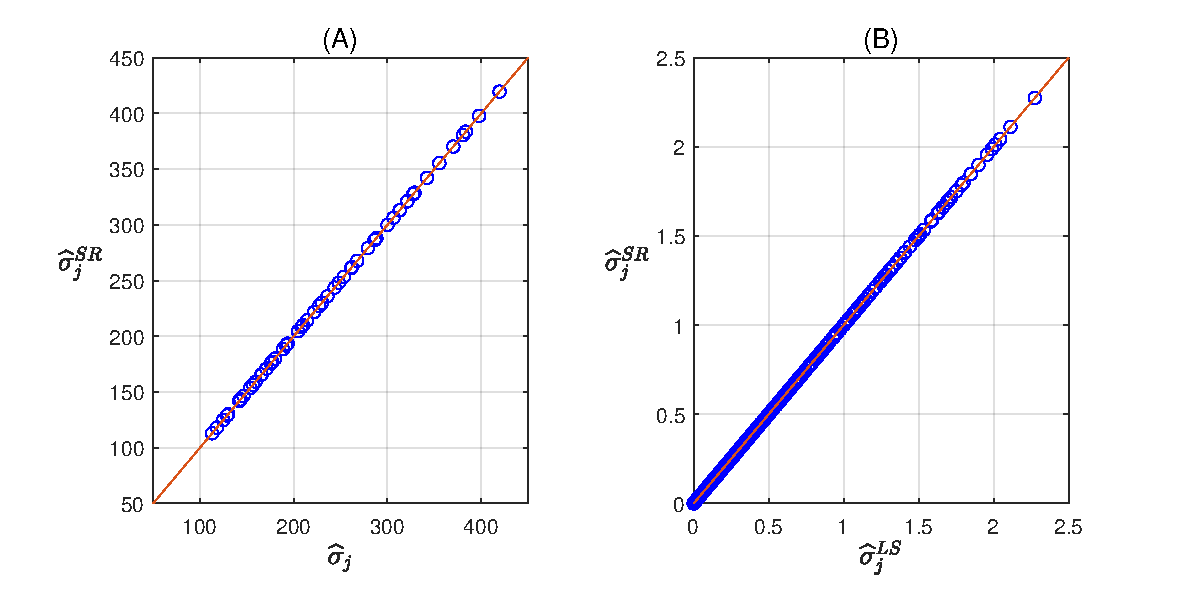
\includegraphics[width=120mm]{Figure/Fig2.pdf}
  \centering
  \caption{ Under non-orthogonal $\boldsymbol{X}$, panel (A) displays the plot of the first $50$ singular values of $\widehat{\boldsymbol{\Theta}}$ versus $\widehat{\boldsymbol{\Theta}}^{\text{SR}}$.
  Panel (B) exhibits the plot of the remaining $200$ singular values of $\widehat{\boldsymbol{\Theta}}^{\text{LS}}$ versus $\widehat{\boldsymbol{\Theta}}^{\text{SR}}$.}
  \label{Fig2}
\end{figure}

Note that as long as $\widehat{\boldsymbol{\Theta}}^{\text{LS}}$ is a full-rank, $\widehat{\boldsymbol{\Theta}}^{\text{SR}}$ is a full-rank matrix whose first $\widehat{r}$ singular values are identical to those of $\widehat{\boldsymbol{\Theta}}$, and remaining $(p-\widehat{r})$ singular values are equal to the  corresponding singular values of $\widehat{\boldsymbol{\Theta}}^{\text{LS}}$.
Although the result of Proposition~\ref{surrogate} is stated under orthogonal design assumption, we also empirically demonstrate that the same results hold under non-orthogonal design in Figure~\ref{Fig2}.
Specifically, under the same experimental setting of Figure~\ref{Fig1}, $\widehat{\boldsymbol{\Theta}}$ is a minimizer of~\eqref{WMVR} obtained via WMVR-ADMM with the weight updating scheme, which will be introduced in Section~\ref{parameter_selection}.
In this experiment, the minimum absolute off-diagonal entry of $\boldsymbol{X}^{\top}\boldsymbol{X}$ is $0.00157$, which implies $\boldsymbol{X}$ is a non-orthogonal design.
The result in Figure~\ref{Fig2} is consistent with the statement in Proposition~\ref{surrogate}.

\subsection{GCV Statistic and Weight Updates}
We divide the process for tuning $\boldsymbol{\lambda_{n}}$ and weights $\omega_{1}, \cdots, \omega_{p}$ into two procedures.
In the first procedure, we propose a following iterative algorithm that alternates between estimating $\boldsymbol{\Theta}^{\star}$ and updating weights.
\begin{enumerate}
    \item[(I)] Set the iteration count $\ell$ to $0$ and weights $\omega_{1}^{(0)}=\dots=\omega_{p}^{(0)}=1$.
    \item[(II)] For the fixed $\boldsymbol{\lambda}_{n}$, solve~\eqref{WMVR} via WMVR-ADMM with the weights $\{\omega_{j}^{(\ell)}\}_{j=1}^{p}$, and denote the solution as  $\widehat{\boldsymbol{\Theta}}^{(\ell)}$.
    \item[(III)] Update weights : for each $j\in\{1,\dots,p\}$,
    \begin{align} \label{weight}
        \omega_{j}^{(\ell+1)}=\frac{1}{\sigma_{j}(\widehat{\boldsymbol{\Theta}}^{(\ell)})+\epsilon}.
    \end{align}
    \item[(IV)] Terminate until convergence or when $\ell$ attains a pre-specified maximum number of iterations.
    Otherwise, increment $\ell$ and go to step {\bf(II)}.
\end{enumerate}

The introduced parameter $\epsilon>0$ in step {\bf(III)} guarantees that, for any $j\in\{1,\dots,p\}$,
the $(\ell+1)^{\text{th}}$ updated weight $\omega_{j}^{(\ell+1)}$ is computable, even when $\sigma_{j}(\widehat{\boldsymbol{\Theta}}^{(\ell)})=0$.
The recovery process of $\boldsymbol{\Theta}^{\star}$ is reasonably robust to the choice of $\epsilon$, and we set $\epsilon=10^{-3}$ hereafter.
The choice $\epsilon=10^{-3}$ may appear a little bit arbitrary, but works well in practice. The resulting estimator from the first procedure is denoted by $\boldsymbol{\text{W}}(\boldsymbol{\lambda_{n}})$. We use a superscript $\boldsymbol{\text{W}}$ in $\widehat{\boldsymbol{\Theta}}^{\text{W}}(\boldsymbol{\lambda_{n}})$ to indicate that the estimator is a converged solution from weight updating procedure introduced above, and use $\boldsymbol{\lambda_{n}}$ to denote the estimator is obtained from a fixed hyper-tuning parameter  $\boldsymbol{\lambda_{n}}$.

The second procedure is designed for choosing parameter $\boldsymbol{\lambda_{n}}$. We develop a GCV type of statistic~\citep{golub1979generalized}, which is more computationally efficient than the ordinary CV (Cross Validation) method, especially in large scale problems. This can be done by using the surrogate estimator $\widehat{\boldsymbol{\Theta}}^{\text{SR}}$ for approximating the degrees of freedom of $\widehat{\boldsymbol{\Theta}}^{\text{W}}(\boldsymbol{\lambda_{n}})$ from the first procedure. That is, given $\widehat{\boldsymbol{\Theta}}^{\text{W}}(\boldsymbol{\lambda_{n}})$, we can construct $\boldsymbol{K}^{\text{W}}$ from (\ref{K}).
Then, by proposition \ref{surrogate}, we can define the projection matrix (hat matrix) for the regression problem~\eqref{closed_form} by $\boldsymbol{X} \big(\boldsymbol{X}^{\top}\boldsymbol{X}+\boldsymbol{\lambda}_{n}n\boldsymbol{K}^{\text{W}}\big)^{-1}\boldsymbol{X}^{\top}$ and approximate the degrees of freedom of $\widehat{\boldsymbol{\Theta}}^{\text{W}}(\boldsymbol{\lambda_{n}})$ as
\begin{align}
    \text{df}(\boldsymbol{\lambda}_{n}) \approx d_{2} \textbf{tr}\big(\boldsymbol{X} \big(\boldsymbol{X}^{\top}\boldsymbol{X}+\boldsymbol{\lambda}_{n}n\boldsymbol{K}^{\text{W}}\big)^{-1}\boldsymbol{X}^{\top}\big).
\end{align}
Thus, the GCV score for $\widehat{\boldsymbol{\Theta}}^{\text{W}}(\lambda_{n})$ is given by
\begin{align} \label{GCV}
    \text{GCV}(\boldsymbol{\lambda}_{n}) := \frac{\textbf{tr}\big(\big(\boldsymbol{Y}-\boldsymbol{X}\widehat{\boldsymbol{\Theta}}^{\text{W}}(\lambda_{n})\big)\big(\boldsymbol{Y}-\boldsymbol{X}\widehat{\boldsymbol{\Theta}}^{\text{W}}(\lambda_{n})\big)^{\top}\big)}{d_{1}d_{2}-\text{df}(\boldsymbol{\lambda}_{n})},
\end{align}
and the optimal $\boldsymbol{\lambda}_{n}^{\star}$ for which GCV($\boldsymbol{\lambda}_{n}$) is obtained by minimizing the GCV score (\ref{GCV}) over the search range $\boldsymbol{\lambda}_{n}\in [0,\mathcal{T}]$.

\section{Simulation Study} \label{SC5}
In subsection $5.1$, we empirically demonstrate convergence results stated in Theorem~\ref{convergence}.
In subsection $5.2$, we compare our methods with the existing methods in terms of estimation error.
Specifically, SNN method (\citet{yuan2007dimension}) and the estimator introduced by~\citet{chen2013reduced} are used for the comparisons.
Hereafter, we refer the estimator in~\citet{chen2013reduced} as Adpative Nuclear Norm estimator (i.e., ANN estimator).
Moreover, we provide an experiment showing the effectiveness of our weight updating scheme~\eqref{weight} in comparison to weight setting in~\citet{chen2013reduced}.

\subsection{Convergence of WMVR-ADMM} \label{conv_exp}
The convergences of WMVR-ADMM can be observed through the following two quantities:
\begin{enumerate}
    \item For checking the Primal residual convergence (i.e., $\boldsymbol{\Theta}^{(k)}-\boldsymbol{\Gamma}^{(k)}\rightarrow{0}$ as $k\rightarrow{\infty}$),
    and $\boldsymbol{\Gamma}^{(k)}$ convergence (i.e., $\boldsymbol{\Gamma}^{(k+1)}-\boldsymbol{\Gamma}^{(k)}\rightarrow{0}$ as $k\rightarrow{\infty}$), we consider
    \begin{align*}
        R^{(k)} := \| \boldsymbol{\Theta}^{(k)}-\boldsymbol{\Gamma}^{(k)} \|_{\text{F}}^{2} +
        \| \boldsymbol{\Gamma}^{(k+1)}-\boldsymbol{\Gamma}^{(k)} \|_{\text{F}}^{2}.
    \end{align*}
    \item For checking the objective convergence, we consider
    \begin{align*}
        O^{(k)} :=  \frac{1}{2n} \left\| \boldsymbol{Y}-\boldsymbol{X}\boldsymbol{\Theta}^{(k)} \right\|_{\text{F}}^{2} + \boldsymbol{\lambda}_{n} \left\| \boldsymbol{\Theta}^{(k)}\right\|_{\boldsymbol{\omega,\star}} .
    \end{align*}
\end{enumerate}

\begin{figure} [t!]
  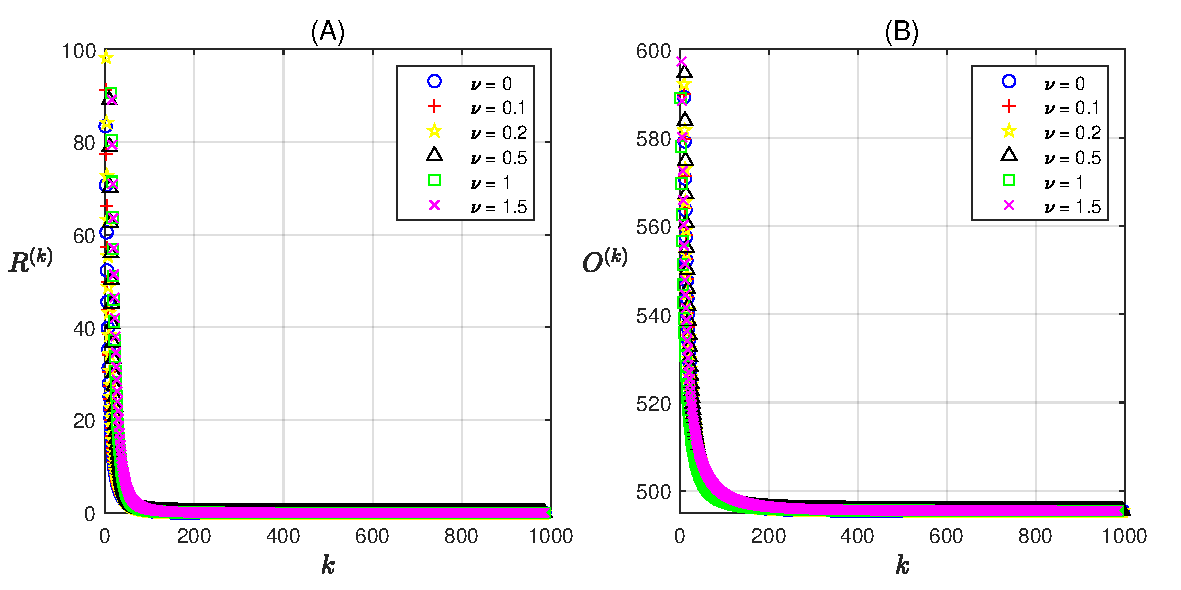
\includegraphics[width=120mm]{Figure/Fig4.pdf}
  \centering
  \caption{Convergences of $R^{(k)}$ (panel (A)) and $O^{(k)}$ (panel (B)) over the algorithm iteration index $k$.
  Regardless of random initializations, $R^{(k)}$ and $O^{(k)}$ converge to $0$ and to a same objective function value, respectively.}
  \label{Fig4}
\end{figure}

Under the exactly same simulation setting as that from the experiment for Figure~\ref{Fig1} with $n=250$, we vary the initialized tuple matrix values $(\boldsymbol{\Theta}^{(0)},\boldsymbol{\Gamma}^{(0)},\boldsymbol{\Lambda}^{(0)})$ of WMVR-ADMM in Algorithm \ref{alg:1}. 
Entries of three matrices are sampled from $\mathcal{N}(0,\nu^{2})$, where $\nu=\{0,0.1,0.2,0.5,1,1.5\}$. 
Weights $\{\omega_j\}_{j=1}^{p}$ are updated once, and with the updated weights, $R^{(k)}$ and $O^{(k)}$ are calculated with the same data set $(\boldsymbol{X},\boldsymbol{Y})$ over all simulation scenarios. 
The resulting  $R^{(k)}$ and $O^{(k)}$ values are demonstrated in Figure~\ref{Fig4}, and the figure shows that both $R^{(k)}$ and $O^{(k)}$ converge to 0 as $k$ increases, regardless of the initializations of algorithm.  
This observation is consistent with the claims in Theorem~\ref{convergence}, and implies that the the converged solutions from WMVR-ADMM have the same objective value on the non-convex landscape of problem~\eqref{WMVR}.

\subsection{Comparisons of Estimation Error with Other Methods}

The simulation setting is under model (\ref{MVR}) with a ground-truth coefficient matrix $\boldsymbol{\Theta}^{\star}$  whose dimension is $d_{1} = 25$ and $d_{2} = 25$.
The coefficient matrix is generated by choosing $\boldsymbol{\Theta}^{\star}  = \boldsymbol{A}\boldsymbol{B}^{\top},$ where $\boldsymbol{A}, \boldsymbol{B} \in R^{25 \times r^{\star}}$ and the elements of  $\boldsymbol{A}$ and $\boldsymbol{B}$ are independently and identically following the standardized normal distribution $\mathcal{N}(0, 1)$.
The value $r^{\star}$ is the rank of the ground truth matrix and is chosen to be $2, 5, 8,$ and $11$.
The design matrix $\boldsymbol{X}$ are chosen randomly from a normal distribution $\mathcal{N}(0, \mathcal{I}_{ d_{1} \times d_{1}})$, and the noise matrix $\boldsymbol{E}$ are independently chosen from another $\mathcal{N}(0, \mathcal{I}_{ d_{2} \times d_{2}})$.
The sample sizes $n$ are set to be 30, 300, and 3000, and the simulation is repeated 100 times.

The estimation errors of the proposed method are recorded in terms of the root mean squared errors (RMSE) between the estimated coefficient matrix and the ground-truth matrix for each simulation.
The results are compared with those from SNN and ANN methods.
Recall SNN estimator is equivalent to the model~\eqref{MVR} with $\{\omega_{j}\}_{j=1}^{p}$.
As for ANN estimator, let $\widehat{\boldsymbol{U}}^{\text{XLS}}\widehat{\boldsymbol{D}}^{\text{XLS}}\big(\widehat{\boldsymbol{V}}^{\text{XLS}}\big)^{\top}$ be SVD of the matrix $\boldsymbol{X}\widehat{\boldsymbol{\Theta}}^{\text{LS}}:=\boldsymbol{X}\big(\boldsymbol{X}^{\top}\boldsymbol{X}\big)^{-1}\boldsymbol{X}^{\top}\boldsymbol{Y}$.
Then, the estimator (Corollary 1 in~\citet{chen2013reduced}) has a closed-form solution as:
\begin{align}
    \widehat{\boldsymbol{\Theta}}^{\text{ANN}} = \widehat{\boldsymbol{\Theta}}^{\text{LS}}
    \widehat{\boldsymbol{V}}^{\text{XLS}} \big(\widehat{\boldsymbol{D}}^{\text{XLS}}\big)^{-1}
    \mathcal{S}_{\boldsymbol{\lambda}_{n}\omega}\big(\widehat{\boldsymbol{D}}^{\text{XLS}}\big)
    \big(\widehat{\boldsymbol{V}}^{\text{XLS}}\big)^{\top},
\end{align}
where $\mathcal{S}_{\boldsymbol{\lambda}_{n}\omega}\big(\widehat{\boldsymbol{D}}^{\text{XLS}}\big)=\text{diag}\bigg\{\max\bigg\{\sigma_{j}(\widehat{\boldsymbol{D}}^{\text{XLS}})-\boldsymbol{\lambda}_{n} w_{j},0 \bigg\}$ for $j=1,\dots,p\bigg\}$. The three methods WMVR-ADMM, SNN, and WNN include parameters needed to be tuned, and we use the GCV tuning method from Section 4 for the tuning.

All results are demonstrated in Figure~\ref{Fig_S4_Ex1}.
The first row of Figure~\ref{Fig_S4_Ex1} shows the performance of all methods under the case whose ground-truth matrix is rank 2 ($r^{\star} = 2$), and we observe that the averages of RMSEs from the WMVR-ADMM method are smaller than those from other methods for all sample size cases.
The second to fourth rows of Figures~\ref{Fig_S4_Ex1} presents the RMSE results from rank $r^{\star} = 5, 8$, and $11$ cases, and the proposed methods are still better than other methods in almost all cases.
Additionally, the panels in Figure~\ref{Fig_S4_Ex1} demonstrate that the RMSEs from the proposed estimator decrease to $0$ as the sample size increases.
This shows the consistency property of the proposed estimator empirically.

\begin{figure}[b!]
  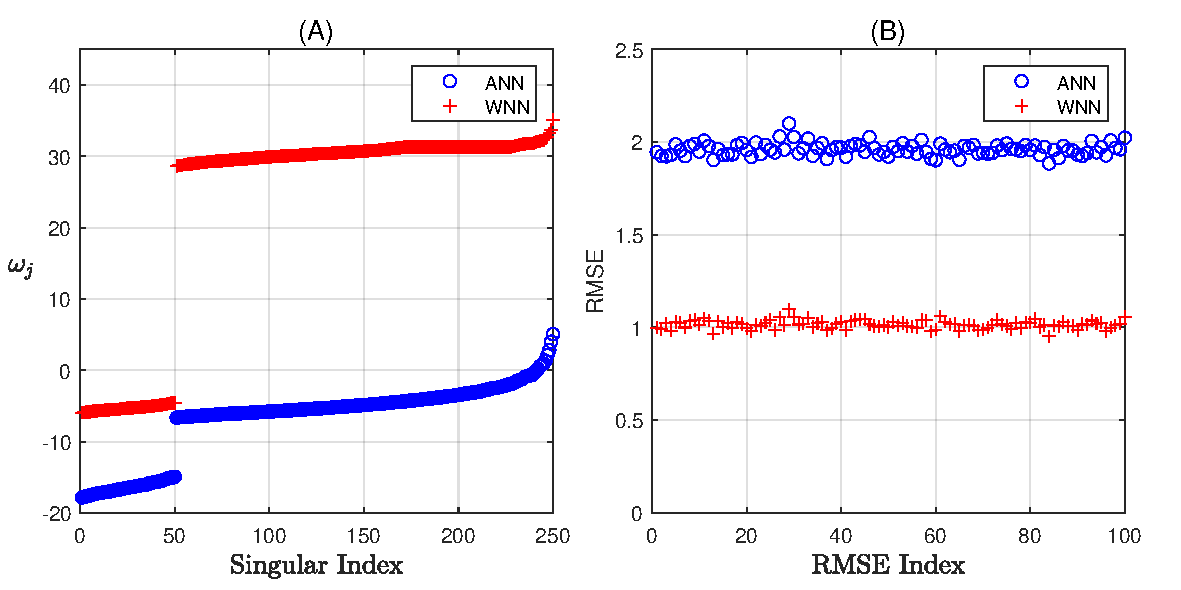
\includegraphics[width=120mm]{Figure/Fig5.pdf}
  \centering
  \caption{Two sequences of weights in (30) used for the estimation (panel (A)) and the resulting RMSEs (panel (B)). Low RMSEs of WNN weights arise from the high penalization on the remaining $200$ singular values, when they are compared with RMSEs of ANN weights.}
  \label{Fig5}
\end{figure}

\begin{figure}[htbp!]
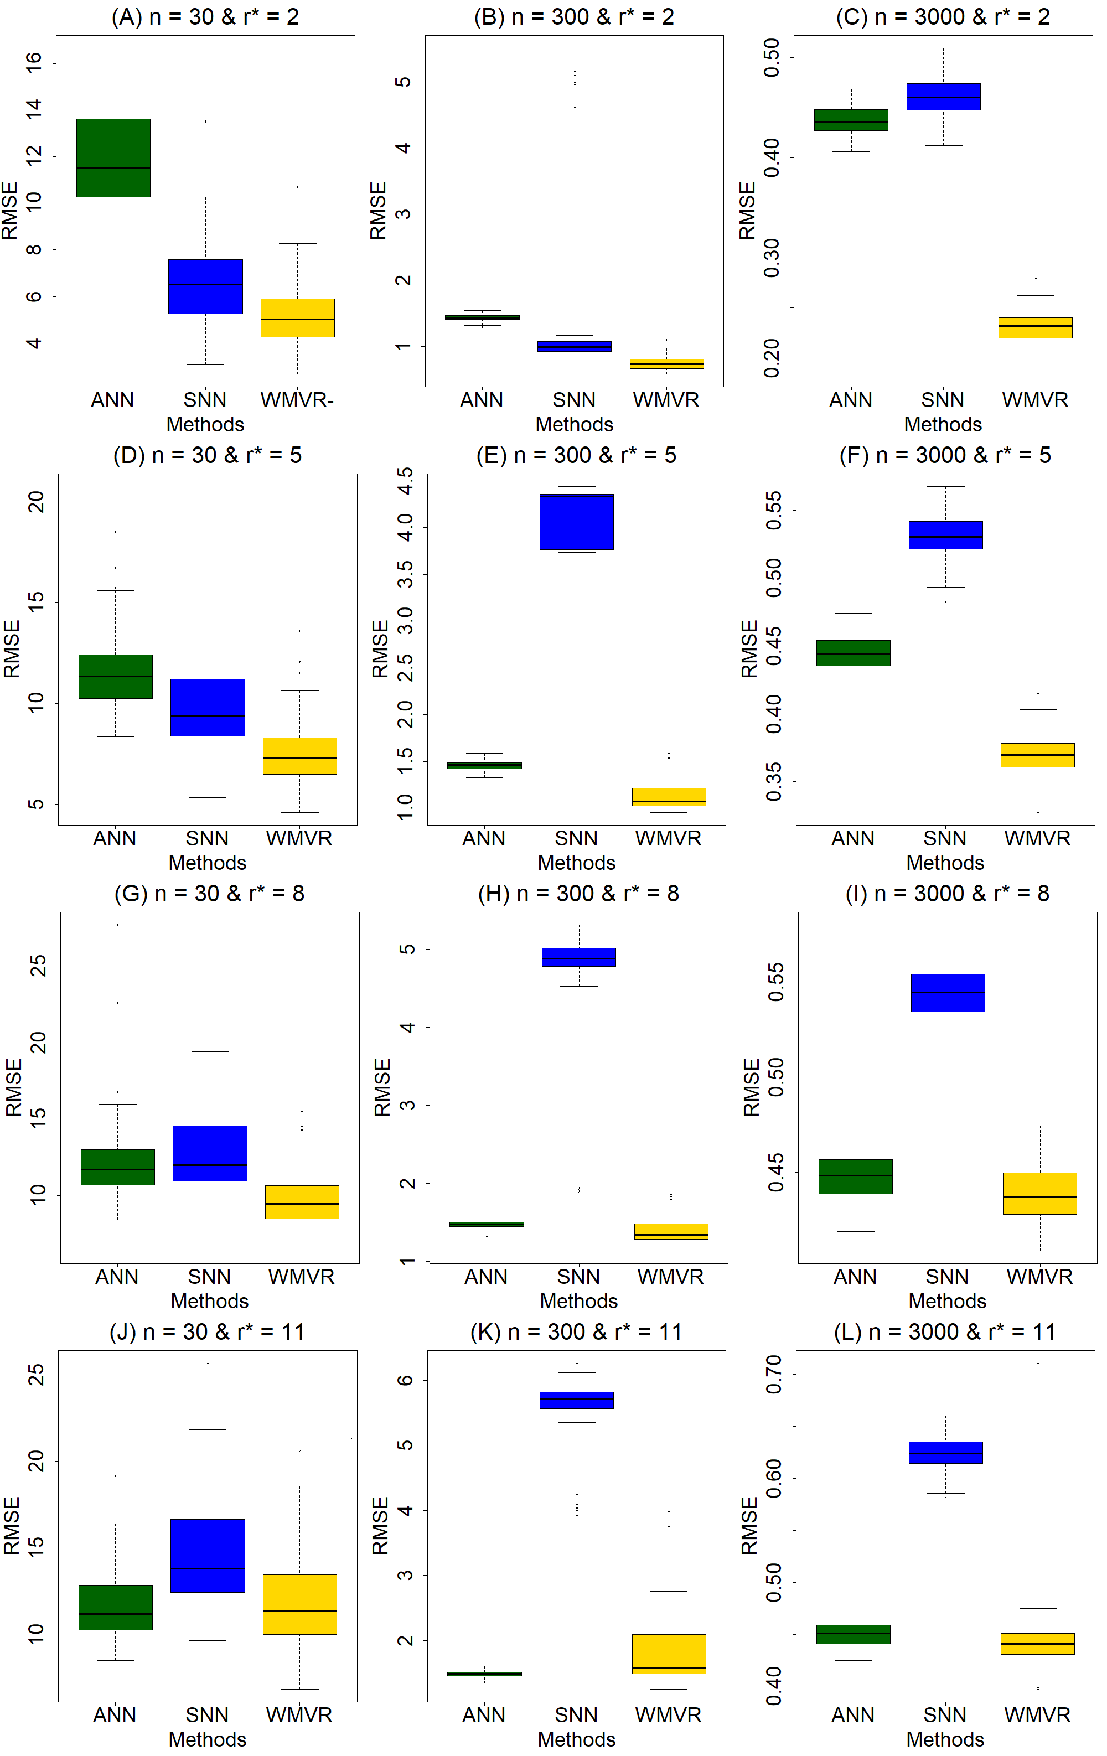
\includegraphics[width=95mm]{Figure/S5_P1.pdf}
\centering
\caption{The plots demonstrates the comparisons of estimation errors in terms of RMSEs from the proposed method with ANN and SNN methods under different simulation settings. 
The three figures in the first row (A) $\sim$ (C) are the comparison results from sample size 30, 300, and 3000, respectively, under the true rank $r^{\star} = 2$. 
Analogously, Figures (D) $\sim$ (F) (second row) are the results from $r^{\star} = 5,$ Figures (G) $\sim$ (I) (third row) are the results from $r^{\star} = 8,$ and Figures (J) $\sim$ (L) (fourth row) are the results from $r^{\star} = 11.$  }
\label{Fig_S4_Ex1}
\end{figure}

To show the effectiveness of the proposed weight updating scheme in section~\ref{parameter_selection},
we compare the weight setting suggested in~\citet{chen2013reduced} with our method.
For the comparison, we revisit the synthetic setting used in Figure~\ref{Fig1}.
Let $\widehat{\boldsymbol{\Theta}}^{(1)}$ be the SNN estimator, and denote $\omega^{\text{WNN}}$
and $\omega^{\text{ANN}}$ be the weight settings introduced in~\eqref{weight} and~\citet{chen2013reduced}, respectively.
Then, we have
\begin{align} \label{weight_comp}
    \omega_{j}^{\text{WNN}} =
    \big(\sigma_{j}(\widehat{\boldsymbol{\Theta}}^{(1)})+10^{-3}\big)^{-1},
    \qquad
    \omega_{j}^{\text{ANN}} =
    \sigma_{j}\big( \boldsymbol{X}\widehat{\boldsymbol{\Theta}}^{\text{LS}} \big)^{-2},
    \qquad j=1,\dots,250.
\end{align}


For the fair comparison, we use WMVR-ADMM estimator.
In Figure~\ref{Fig5}, panel (A) shows the two sequences of averaged weights $\{\omega_{j}\}_{j=1}^{250}$ in~\eqref{weight_comp} used for the estimation in logarithmic scale,
and panel (B) exhibits 100 RMSEs with the respective weight scheme.
While the difference of the first $50$ weights between two weight schemes is negligible, the effect of WNN-weight scheme is dramatized for penalizing the remaining $200$ singular values in comparison to ANN-weight scheme, and this results in lower RMSEs in panel (B).

\section{Application to A Real Dataset}

\begin{figure}[b!]
    \centering
    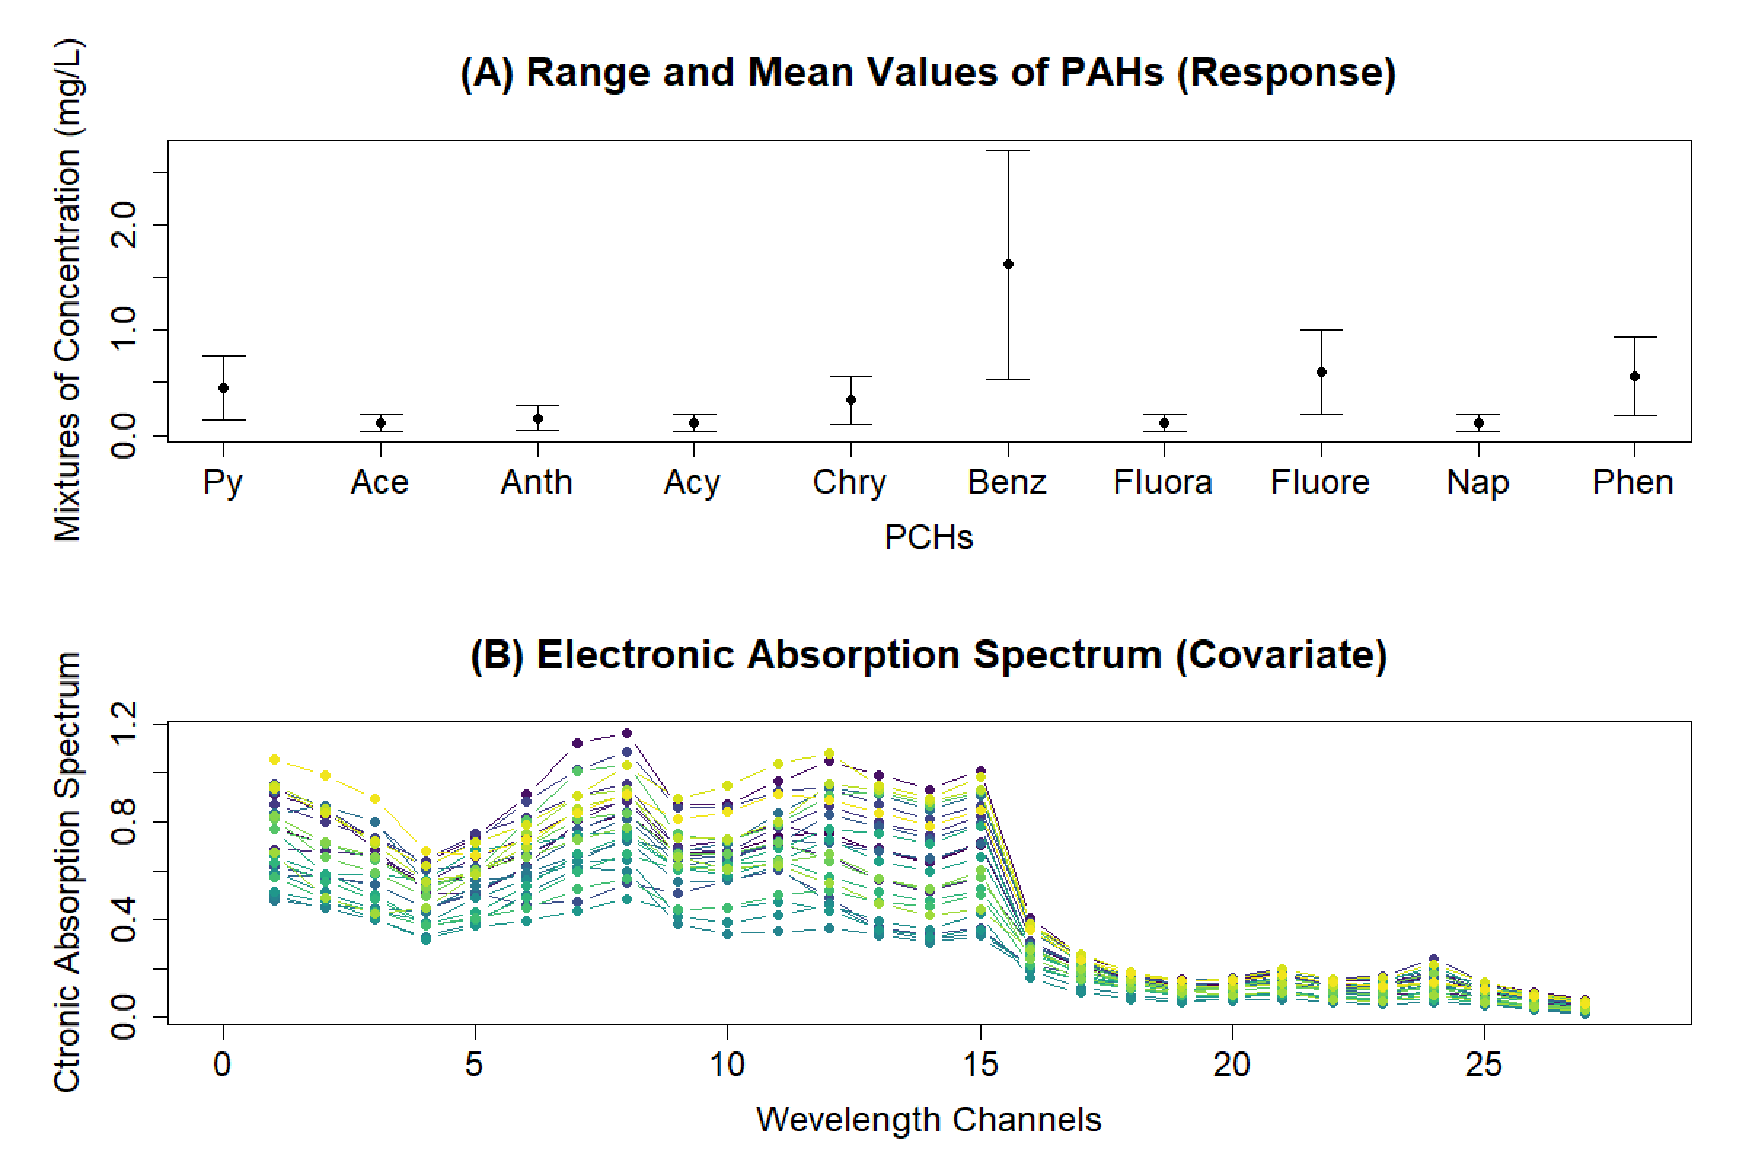
\includegraphics[width = 120mm]{Figure/S6_P1.pdf}
    \caption{Demonstration of the mixture components of the PAHs ($\boldsymbol{Y}$) and the electronic absorption spectrum of the 25 samples ($\boldsymbol{X}$)}
    \label{fig:Realdata_XY}
\end{figure}

Although there are many applications of multivariate linear regression (\ref{MVR}) in the literature, these applications are usually analyzed by assuming a full rank model and least square method for estimating.
In this section, we demonstrate an important application of model (\ref{MVR}) without the full rank assumption through the proposed WMVR-ADMM method.
The application is about a study of Polycyclic Aromatic Hydrocarbons (PAHs) from Section $2.2.2$ of \citet{isenmann2008modern}.

PAHs are ubiquitous environmental contaminants generated primarily during the incomplete combustion of some organic substances, such as coal, oil, rubbish, and wood. They are linked with the causes of tumors and their effects on reproduction. PAHs are widely used in industry or medicines to make dyes, plastics, and pesticides. In the dataset, 10 PAHs, including pyrene (Py), acenaphthene (Ace), anthracene (Anth), acenaphthylene (Acy), chrysene (Chry), benzanthracene (Benz), fluoranthene (Fluora), fluorene (Fluore), naphthalene (Nap), phenanthracene (Phen), and 25 complex mixtures of certain concentrations (with unit milligrams per liter) of these PAHs were recorded, which indicates $n = 25$ and $d_{1} = 10$ in model (\ref{MVR}). The mean and range values of these mixtures of certain concentrations are plotted in Panel (A) of Figure \ref{fig:Realdata_XY}.
From each of these mixtures, an electronic absorption spectrum is computed, The spectrum are digitized at 5 nm intervals 27 wavelength channels from 220 nm to 350 nm, as shown in in Panel (B) of Figure \ref{fig:Realdata_XY}.  This means there are 27 columns for $\boldsymbol{X}_{2}$ in model (\ref{MVR}) ($d_{2}  = 27$). More details about the dataset can be found in Section 5.1.2 of \citet{brereton2003chemometrics} and Section 2.2.2 of \citet{isenmann2008modern}.

\begin{figure}[hbt!]
    \centering
    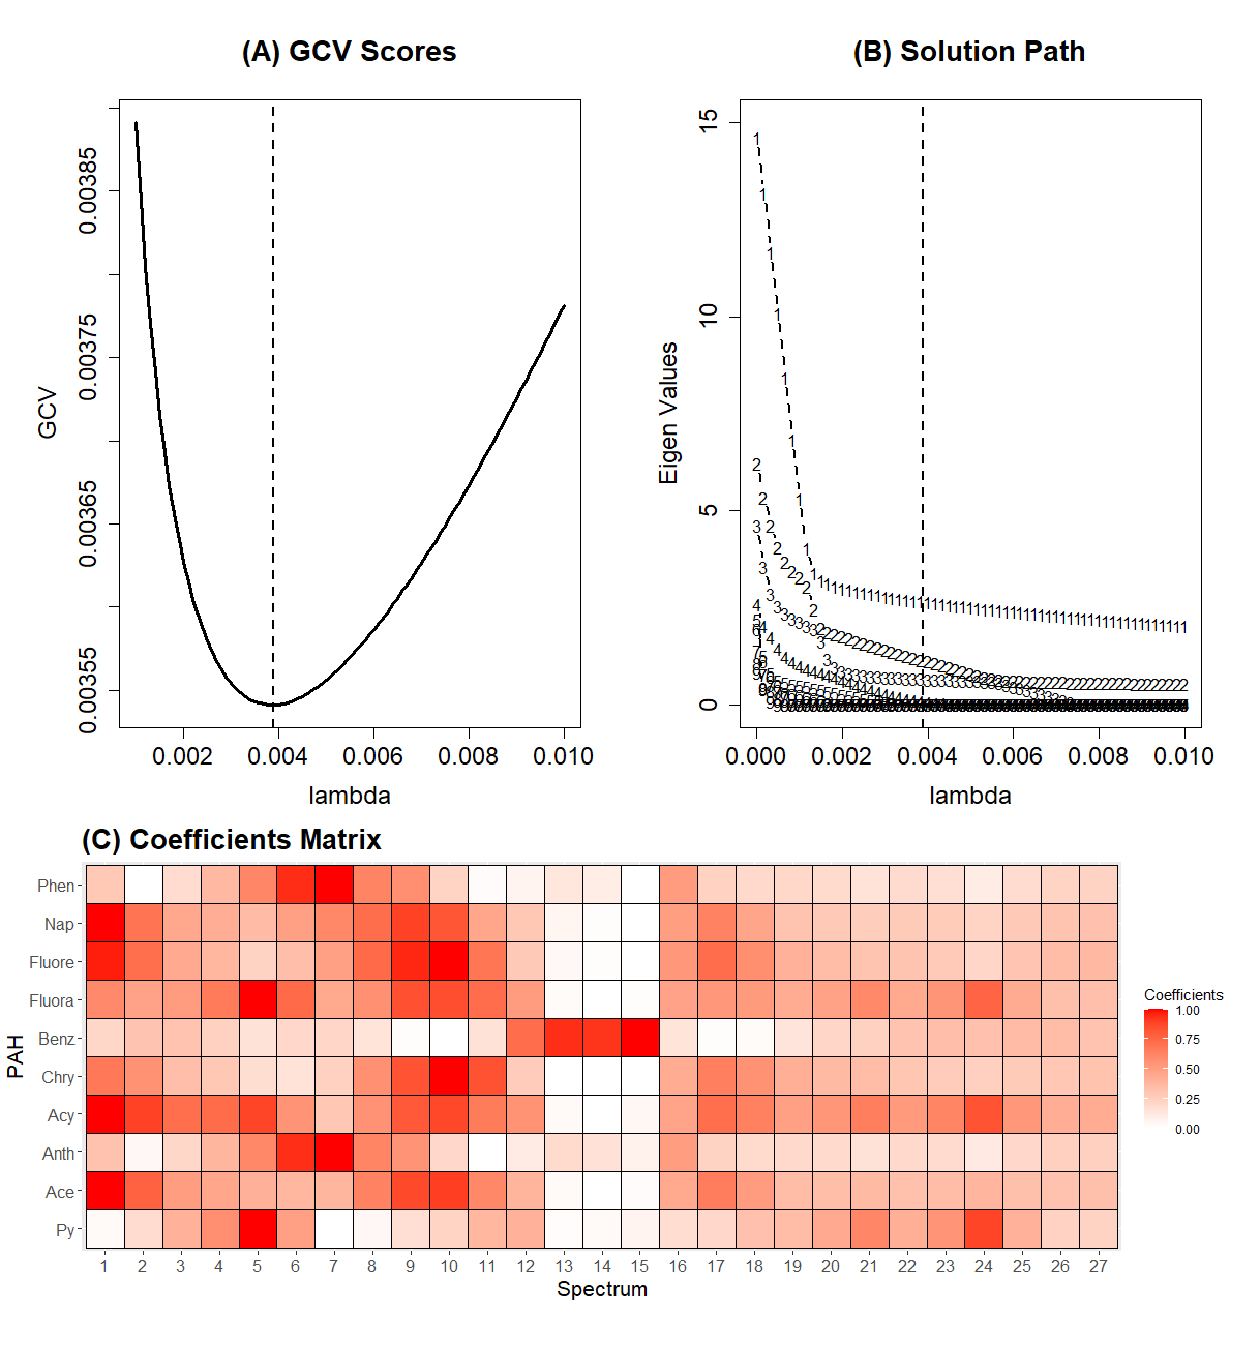
\includegraphics[width = 95mm]{Figure/S6_P2.pdf}
    \caption{(A) GCV Score Versus Tuning Parameters $\boldsymbol{\lambda}$, (B) Solution Path, (C) Estimated Coefficient Matrix.}
    \label{fig:Realdata_GCV}
\end{figure}

We are mainly interested in using WMVR-ADMM to understand the association between the concentrations from PAHs (Figure
\ref{fig:Realdata_XY} (A)) and the electronic absorption spectrum  (Figure \ref{fig:Realdata_XY} (B)) through model (\ref{MVR}). The method is conducted by following Algorithm 1, and the optimal tuning parameter $\boldsymbol{\lambda}_{n}$ and weights $\boldsymbol{w}$ are selected by the proposed GCV criterion described in Section 4.
The resulting GCV scores are plotted in Figure \ref{fig:Realdata_GCV} (A) with respect to value $\boldsymbol{\lambda}_{n}$, showing the selected $\boldsymbol{\lambda}_{n}$ is around $0.039$.
The estimated eigenvalues with respect to $\boldsymbol{\lambda}_{n}$ are plotted in Figure \ref{fig:Realdata_GCV} (B), and under the optimal $\boldsymbol{\lambda}_{n}$ and weights from the GCV criterion, the estimated coefficient matrix is rank $5$.
The estimated coefficients are demonstrated in a heatmap as shown in Figure \ref{fig:Realdata_GCV} (C).
The figure shows that for each PAH, only a few important channels can be used to determine the concentrations because only some coefficients are relatively large.
Additionally, these larger coefficients are usually from smaller column numbers in the heatmap.
Thus, the channels with smaller wavelengths are more important than larger wavelength channels.

\section{Conclusion and Discussion} \label{Disc}
We propose an ADMM-based method for solving the multivariate regression problem with WNN penalty.
Under non-decreasing order of weights, the WNN is a non-convex function, and induce non-convexity of WNN penalized least-square 
problem in~\eqref{MVR} over the parameter space.
The provided algorithm is shown to converge uniquely to one of stationary points of augmented Lagrangian function. 
The statistical properties of the estimator are investigated under orthogonal design, providing some insights on the choices of weights for the estimation.
Furthermore, the minimax convergence rate of the estimation error is derived under random Gaussian design setting.
In simulation studies, we demonstrate followings: 
$(I)$  under random initializations, solutions of~\eqref{WMVR} via WMVR-ADMM algorithm converge to a certain estimator whose objective values are same
$(II)$ the WNN method outperforms SNN~\citep{yuan2007dimension} and ANN~\citep{chen2013reduced} under synthetic settings,
$(III)$ the effect of our suggested weight updating scheme is verified through the comparison with the weight setting by~\citet{chen2013reduced}.
Lastly the application to the real data set shows the effectiveness of our method. 
Nonetheless, there are several remaining open questions which require further investigations in the future.
We summarize them as follows.
\begin{figure} [t!]
  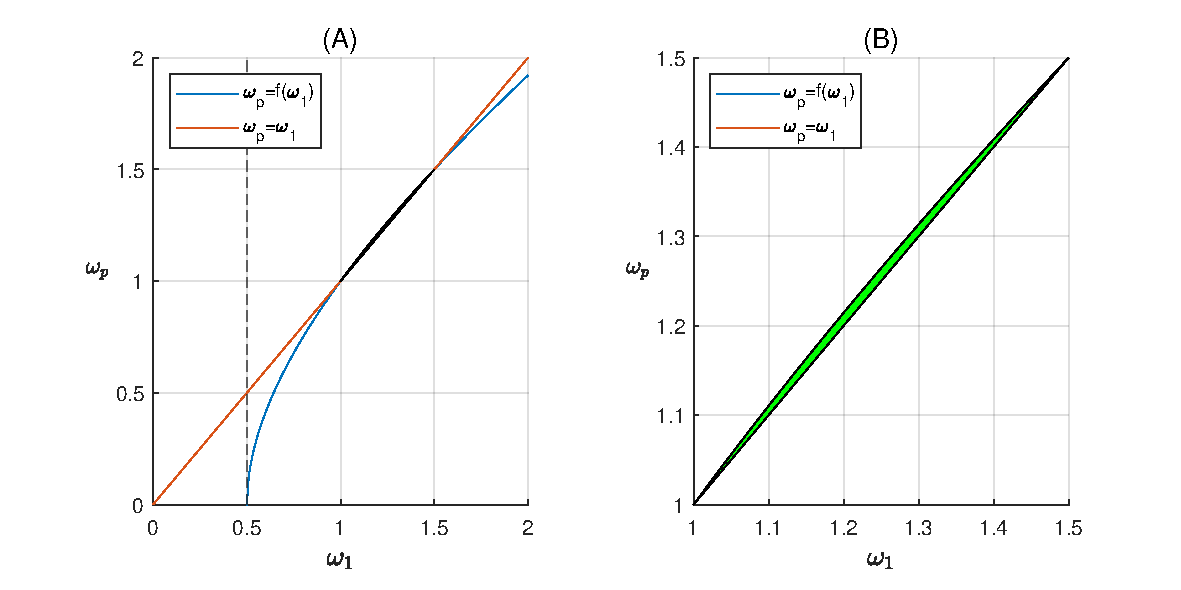
\includegraphics[width=130mm]{Figure/Fig3.pdf}
  \centering
  \caption{ Panel (A) exhibits the intersected region of $\mathcal{W} \leq 3$ and $\frac{1}{2} < \omega_{1} \leq \dots \leq \omega_{p}$. Panel (B) magnifies the intersected region on grid $(\omega_{1},\omega_{p})\in[1,1.5] \times [1,1.5]$. }
  \label{Fig6}
\end{figure}

\begin{enumerate}
    \item A question on whether the non-convex ADMM can achieve the global minimizer of~\eqref{WMVR} is a huge open question.
    Although empirical results on the convergence of WMVR-ADMM are provided in section~\ref{SC5}, they still cannot verify the converged solution is a global minimizer of~\eqref{WMVR}. 
    We leave both empirical and theoretical justifications on this issue as important open problems. 
    Under SNN setting, it is proved that there exists a primal-dual pair of~\eqref{WMVR} which satisfies the strong duality~\citep{shang2021regularization}.
    Therefore, the existence of saddle point on $\mathcal{L}_{0}$ can be ensured, so that the global minimizer of~\eqref{WMVR} can be proved through the classical techniques in~\citet{boyd2011distributed}.
    Nonetheless, we need further investigation whether these conditions can be used under our WNN setting with non-decreasing weights.

    \item As previously mentioned in the remark of Theorem~\ref{thm2}, $\mathcal{W}:= w_{p}\big(2w_{p}-w_{1}+\frac{1}{2}\big)/(w_{1}-\frac{1}{2})$ is a sole factor that accounts for the effects of weights in the convergence rate of~\eqref{Rate}.
    This result naturally leads us to ask the question; ``Under which pair of $(\omega_{1},\omega_{p})$, does the estimator from WNN have a faster convergence rate than the one from SNN?''.
    Under the same choices of tuning parameter $\boldsymbol{\lambda}_{n}$, a naive way for the comparison is to plug $\omega_{1}=\omega_{p}=1$ in $\mathcal{W}$. 
    That is, we want to find a pair of $(\omega_{1},\omega_{p})$ for which $\mathcal{W} \leq 3$ and $\frac{1}{2} < \omega_{1} \leq \dots \leq \omega_{p}$.
    The intersected region is illustrated in Figure~\ref{Fig6}.
    From our empirical experiences, the region of $(\omega_{1},\omega_{p})$, for which WNN is superior than SNN in terms of estimation, is much larger than it is presented in Figure~\ref{Fig6}.
    This problem arises from the tightness of the subset $\mathcal{C}$ we derive in Lemma~\ref{Cone_like_set}.
    In order to avoid this problem, we suspect that the different approach from using RSC condition of cost function is needed.
    A paper~\citet{law2021rank}, recently appeared on arXiv, introduces a technique which takes the advantage of controlling the covering number of projection operators corresponding to the subspaces spanned by the design.
    They consider a problem of solving nuclear norm penalized least square problem, and their technique is independent from RSC condition. 
    It would be an interesting open problem if their technique can be employed in our problem for obtaining a bigger intersected region than that in Figure~\ref{Fig6}.
\end{enumerate}

\bibliography{Ref_all}

\newpage
\section{Appendix}
In this section, an extended algorithm of WMVR-ADMM to trace regression model is proposed in Section 8.1.
%Then, we provide a noition of decomposability of nuclear norm with respect to a pair of specially designed matrix subspaces.
Subsequently, proofs on Lemma~\ref{Lemma2.3}, Lemma~\ref{Lemma2.4}, Theorem~\ref{convergence}, Lemma~\ref{Cone_like_set}, and Theorem~\ref{thm2} are provided in Sections $8.2$, $8.3$, $8.4$, and $8.5$, respectively.

\subsection{Extension of WMVR-ADMM to Trace Regression Model} \label{tr_algo}
First, let us consider a following trace regression problem :
\begin{equation*}
    y_{i} = \textbf{tr}(\boldsymbol{X}^{T}_{i}\boldsymbol{\Theta^\star}) + \varepsilon_{i} \ ,\ i = 1, \cdots, n, \label{eq: TR}
\end{equation*}
where $\boldsymbol{X}_{i} \in \boldsymbol{R}^{d_{1} \times d_{2}}$ is a known measurement matrix for $i = 1, \cdots, n$ and $\big\{\varepsilon_{i}\big\}_{i=1}^{n}\stackrel{\text{i.i.d}}{\sim} \mathcal{N}\big( 0, \sigma^{2} \big)$.
In this subsection, we present an extension of WMVR-ADMM algorithm for solving a following optimization problem.
\begin{equation*}
    \min_{\boldsymbol{\Theta}} \Bigg\{ \frac{1}{2n}\sum^{n}_{i=1} (y_{i} - \textbf{tr}(\boldsymbol{X}^{T}_{i}\boldsymbol{\Theta}))^2 + \boldsymbol{\lambda}_{n} ||\boldsymbol{\Theta}||_{\boldsymbol{\omega,\star}} \Bigg\}. \label{eq: opt}
\end{equation*}
First, let $v(M)\in\mathbb{R}^{d_{1}d_{2}}$ be the vectorized version of matrix $M$ concatenating columns of $M\in\mathbb{R}^{d_{1} \times d_{2}}$ into one column vector, and let us also define an inverse operator $\textbf{Mat} \big[ v(M) \big] := M$.
With this notation, the algorithm is summarized in the Algorithm~\ref{trace_algo}.
\begin{algorithm}[hbt!]
    \textbf{Input} : $\big\{\boldsymbol{X}_{i},y_{i}\big\}_{i=1}^{n}$, $\boldsymbol{\lambda}_{n} \geq 0$. \\
    \textbf{Prelimiaries} : $\boldsymbol{M_{y}x}:=\sum_{i=1}^{n}y_{i}\boldsymbol{X}_{i}$, and
    $\mathcal{A} := \frac{1}{n}\sum_{i=1}^{n} v(\boldsymbol{X}_{i})v(\boldsymbol{X}_{i})^{\top}+\rho\cdot\mathcal{I}_{ d_1d_2 \times d_1d_2}$. \\
    \textbf{Initialization} : $\boldsymbol{\Theta}^{(0)}=\boldsymbol{0}$, $\boldsymbol{\Gamma}^{(0)}=\boldsymbol{0}$, $\boldsymbol{\Lambda}^{(0)}=\boldsymbol{0} \in\mathbb{R}^{d_{1}\times d_{2}}$. \\
    \qquad {\bf Repeat following Steps :} \\
    \qquad \qquad {\bf Step 1.} Let $\boldsymbol{B^{(k)}}:=\frac{1}{n}\boldsymbol{M_{y}x}-\boldsymbol{\Lambda}^{(k)}+\rho \cdot \boldsymbol{\Gamma}^{(k)}$. \quad $\boldsymbol{B^{(k)}}=\boldsymbol{U}^{\textbf{B}}\boldsymbol{D}^{\textbf{B}}\big(\boldsymbol{V^{\textbf{B}}}\big)^{\top}$. (SVD) \\
    \qquad \qquad \qquad \qquad  Set $\mathcal{S}_{\boldsymbol{\lambda}_{n}\omega}\big(\boldsymbol{D}^{\textbf{B}}\big) = \textbf{diag}\bigg\{ \max\bigg\{\frac{1}{\rho}\big(\sigma_{j}(\boldsymbol{B}^{(k)}\big)-\boldsymbol{\lambda}_{n} w_{j}\big),0 \bigg\}$ for $j=1,\dots,p \bigg\}$.  \\
    \qquad \qquad \qquad \qquad $\boldsymbol{\Theta}^{(k+1)} = \boldsymbol{U}^{\textbf{B}} \mathcal{S}_{\boldsymbol{\lambda}_{n}\omega}\big(\boldsymbol{D}^{\textbf{B}}\big) \big(\boldsymbol{V^{\textbf{B}}}\big)^{\top}$.  \\
    \qquad \qquad {\bf Step 2.}
    $\boldsymbol{\Gamma}^{(k+1)} = \textbf{Mat} \big[\mathcal{A}^{-1}\big(\rho v(\boldsymbol{\Theta}^{(k+1)})-v(\boldsymbol{\Lambda}^{(k)})\big)\big].$\\
    \qquad \qquad {\bf Step 3.} $\boldsymbol{\Lambda}^{(k+1)} = \boldsymbol{\Lambda}^{(k)} + \rho\big( \boldsymbol{\Theta}^{(k+1)}-\boldsymbol{\Gamma}^{(k+1)} \big)$.\\
    \qquad {\bf Until} $|| \boldsymbol{\Theta}^{(k+1)}-\boldsymbol{\Gamma}^{(k+1)} ||_{F}\leq 10^{-7}$ and $|| \boldsymbol{\Gamma}^{(k+1)}-\boldsymbol{\Gamma}^{(k)} ||_{F}\leq 10^{-7}$. \\
    \textbf{Output} : $\widehat{\boldsymbol{\Theta}}=\boldsymbol{\Theta}^{(k+1)}$.
    \caption{ADMM for weighted Trace Regression. (WTR-ADMM)}
    \label{trace_algo}
\end{algorithm}
The presented algorithm can be derived easily by using exactly the same techniques employed in subsection~\ref{WMVR-ADMM} by plugging $f(\boldsymbol{\Theta}):=-\frac{1}{n}\textbf{tr}\big( \big(\sum_{j=1}^{n}y_{i}\boldsymbol{X}_{i}\big)^{\top}\boldsymbol{\Theta} \big)+\boldsymbol{\lambda}_{n}||\boldsymbol{\Theta}||_{\boldsymbol{\omega,\star}}$ and $g(\boldsymbol{\Gamma})=\frac{1}{2n}\sum_{j=1}^{n}\textbf{tr}\big(\boldsymbol{X_i^\top}\boldsymbol{\Gamma}\big)^{2}$ in~\eqref{reform},
and we omit the detailed derivation.

\subsection{Proof of Lemma 3}
By the result of Lemma~\ref{Lemma2.1}, we have
\begin{align} \label{ineq1}
    \mathcal{L}_{\rho} \big( \boldsymbol{\Theta}^{(k)},\boldsymbol{\Gamma}^{(k)},\boldsymbol{\Lambda}^{(k)} \big) 
    - \mathcal{L}_{\rho} \big( \boldsymbol{\Theta}^{(k+1)},\boldsymbol{\Gamma}^{(k)},\boldsymbol{\Lambda}^{(k)} \big)
    \geq 0.
\end{align}
Now, we control the following difference term.
\begin{align} \label{ineq2}
    &\mathcal{L}_{\rho} \big( \boldsymbol{\Theta}^{(k+1)},\boldsymbol{\Gamma}^{(k)},\boldsymbol{\Lambda}^{(k)} \big) - \mathcal{L}_{\rho} \big( \boldsymbol{\Theta}^{(k+1)},\boldsymbol{\Gamma}^{(k+1)},\boldsymbol{\Lambda}^{(k)} \big) \nonumber \\
    &\qquad = g(\boldsymbol{\Gamma}^{(k)})-g(\boldsymbol{\Gamma}^{(k+1)}) - \textbf{tr}\big( \boldsymbol{\Lambda}^{(k)\top}\big(\boldsymbol{\Gamma}^{(k)}-\boldsymbol{\Gamma}^{(k+1)}\big)\big) \nonumber \\
    &\qquad \qquad - \rho \cdot \textbf{tr}\big( \big(\boldsymbol{\Theta}^{(k+1)}-\boldsymbol{\Gamma}^{(k+1)}\big)^{\top}
    \big(\boldsymbol{\Gamma}^{(k)}-\boldsymbol{\Gamma}^{(k+1)}\big) \big) + \frac{\rho}{2}\left\| \boldsymbol{\Gamma}^{(k)}-\boldsymbol{\Gamma}^{(k+1)} \right\|_{F}^{2}  \nonumber \\
    &\qquad = g(\boldsymbol{\Gamma}^{(k)})-g(\boldsymbol{\Gamma}^{(k+1)}) - \textbf{tr}\big( \boldsymbol{\Lambda}^{(k+1)\top}\big(\boldsymbol{\Gamma}^{(k)}-\boldsymbol{\Gamma}^{(k+1)}\big)\big) + \frac{\rho}{2}\left\| \boldsymbol{\Gamma}^{(k)}-\boldsymbol{\Gamma}^{(k+1)} \right\|_{F}^{2}.
\end{align}
Note that we use $\boldsymbol{\Lambda}^{(k+1)}=\boldsymbol{\Lambda}^{(k)}+\rho\big(\boldsymbol{\Theta}^{(k+1)}-\boldsymbol{\Gamma}^{(k+1)}\big)$ in the last equality.
Recall the definition of $\mathcal{L}_{\rho} \big( \boldsymbol{\Theta}^{(k)},\boldsymbol{\Gamma}^{(k)},\boldsymbol{\Lambda}^{(k)} \big)$ from~\eqref{Lagrangian} and $\boldsymbol{\Lambda}^{(k+1)}=\boldsymbol{\Lambda}^{(k)}+\rho\big(\boldsymbol{\Theta}^{(k+1)}-\boldsymbol{\Gamma}^{(k+1)}\big)$.
Then, we have
\begin{align} \label{ineq3}
    \mathcal{L}_{\rho} \big( \boldsymbol{\Theta}^{(k+1)},\boldsymbol{\Gamma}^{(k+1)},\boldsymbol{\Lambda}^{(k)} \big) 
    - \mathcal{L}_{\rho} \big( \boldsymbol{\Theta}^{(k+1)},\boldsymbol{\Gamma}^{(k+1)},\boldsymbol{\Lambda}^{(k+1)} \big) 
    = -\frac{1}{\rho}\left\| \boldsymbol{\Lambda}^{(k)}-\boldsymbol{\Lambda}^{(k+1)} \right\|_{F}^{2}.
\end{align}
By combining~\eqref{ineq2} and~\eqref{ineq3}, we have
\begin{align} \label{ineq4}
    &\mathcal{L}_{\rho} \big( \boldsymbol{\Theta}^{(k+1)},\boldsymbol{\Gamma}^{(k)},\boldsymbol{\Lambda}^{(k)} \big) 
    - \mathcal{L}_{\rho} \big( \boldsymbol{\Theta}^{(k+1)},\boldsymbol{\Gamma}^{(k+1)},\boldsymbol{\Lambda}^{(k+1)} \big) \nonumber \\
    &\qquad = g(\boldsymbol{\Gamma}^{(k)})-g(\boldsymbol{\Gamma}^{(k+1)}) - \textbf{tr}\big( \boldsymbol{\Lambda}^{(k+1)\top}\big(\boldsymbol{\Gamma}^{(k)}-\boldsymbol{\Gamma}^{(k+1)}\big)\big) \nonumber \\
    &\qquad \qquad \qquad \qquad \qquad \qquad \qquad
    + \frac{\rho}{2}\left\| \boldsymbol{\Gamma}^{(k)}-\boldsymbol{\Gamma}^{(k+1)} \right\|_{F}^{2} -\frac{1}{\rho}\left\| \boldsymbol{\Lambda}^{(k)}-\boldsymbol{\Lambda}^{(k+1)} \right\|_{F}^{2}.
\end{align}
Recall the definition of $\boldsymbol{\Gamma}^{(k+1)}$ from \textbf{Step 2} of WMVR-ADMM.
\begin{align*}
    \boldsymbol{\Gamma}^{(k+1)} = \argmin_{\boldsymbol{\Gamma} \in \mathbb{R}^{d_{1} \times d_{2}}}
    \bigg\{ g(\boldsymbol{\Gamma}) - \textbf{tr}\big(\boldsymbol{\Lambda}^{(k)\top}\boldsymbol{\Gamma}\big)+\frac{\rho}{2}\left\|\boldsymbol{\Gamma}-\boldsymbol{\Theta}^{(k+1)} \right\|_{F}^{2} \bigg\}.
\end{align*}
Since $\boldsymbol{\Gamma}^{(k+1)}$ is a stationary point of the above optimization problem, we have
\begin{align*}
    \nabla g\big( \boldsymbol{\Gamma}^{(k+1)} \big)
    = \boldsymbol{\Lambda}^{(k)} + \rho\big( \boldsymbol{\Theta}^{(k+1)}-\boldsymbol{\Gamma}^{(k+1)} \big)
    = \boldsymbol{\Lambda}^{(k+1)},
\end{align*}
where $\nabla g (\cdot)$ is a gradient of $g$.
Likewise, we get $\nabla g\big( \boldsymbol{\Gamma}^{(k)} \big) = \boldsymbol{\Lambda}^{(k)}$.
Recall the definition of $g(\cdot)$, then we can easily have
\begin{align} \label{ineq5}
    \left\|\boldsymbol{\Lambda}^{(k+1)}-\boldsymbol{\Lambda}^{(k)}\right\|_{F} =
    \left\|\nabla g\big( \boldsymbol{\Gamma}^{(k+1)} \big)
    - \nabla g\big( \boldsymbol{\Gamma}^{(k)} \big)\right\|_{F}
    \leq \sigma_{1}\bigg( \frac{1}{n}\boldsymbol{X}^{\top}\boldsymbol{X}\bigg)
    \cdot 
    \left\| \boldsymbol{\Gamma}^{(k+1)} - \boldsymbol{\Gamma}^{(k)} \right\|_{F}.
\end{align}
Function $g$ is Lipschitz smooth with constant $L_{\nabla g}:=\sigma_{1}\bigg( \frac{1}{n}\boldsymbol{X}^{\top}\boldsymbol{X}\bigg)$.
Then, we have 
\begin{align} \label{ineq6}
    g(\boldsymbol{\Gamma}^{(k)}) - g(\boldsymbol{\Gamma}^{(k+1)})
    - \textbf{tr}\bigg(\nabla g\big(\boldsymbol{\Gamma}^{(k+1)}\big)^\top
    \big(\boldsymbol{\Gamma}^{(k)}-\boldsymbol{\Gamma}^{(k+1)}\big)\bigg) \geq -\frac{L_{\nabla g}}{2}
    \left\| \boldsymbol{\Gamma}^{(k+1)} - \boldsymbol{\Gamma}^{(k)} \right\|_{F}^{2}.
\end{align}
Recall $\nabla g\big( \boldsymbol{\Gamma}^{(k+1)} \big) = \boldsymbol{\Lambda}^{(k+1)}$, combining~\eqref{ineq1},~\eqref{ineq4},~\eqref{ineq5}, and~\eqref{ineq6} yields 
\begin{align*}
    \mathcal{L}_{\rho} \big( \boldsymbol{\Theta}^{(k)},\boldsymbol{\Gamma}^{(k)},\boldsymbol{\Lambda}^{(k)} \big) 
    - \mathcal{L}_{\rho} \big( \boldsymbol{\Theta}^{(k+1)},\boldsymbol{\Gamma}^{(k+1)},\boldsymbol{\Lambda}^{(k+1)} \big)
    \geq \bigg(  -\frac{L_{\nabla g}}{2} -\frac{1}{\rho} L_{\nabla g}^{2} + \frac{\rho}{2} \bigg) \cdot 
    \left\| \boldsymbol{\Gamma}^{(k+1)} - \boldsymbol{\Gamma}^{(k)} \right\|_{F}^{2}.
\end{align*}
Setting $\rho>2L_{\nabla g}$ makes $C_{1}:=-\frac{L_{\nabla g}}{2} -\frac{1}{\rho} L_{\nabla g}^{2} + \frac{\rho}{2}>0$, which implies that $\mathcal{L}_{\rho}\big( \boldsymbol{\Theta}^{(k)},\boldsymbol{\Gamma}^{(k)},\boldsymbol{\Lambda}^{(k)} \big)$ is non-increasing over $k\in\mathbb{R}\cup \{0\}$.
Now, we will prove $ \mathcal{L}_{\rho}\big(\boldsymbol{\Theta}^{(k)},\boldsymbol{\Gamma}^{(k)},\boldsymbol{\Lambda}^{(k)}\big)$ is bounded below over $k\in\mathbb{N}\cup\{0\}$.
\begin{align*}
    \mathcal{L}_{\rho}\big(\boldsymbol{\Theta}^{(k)},\boldsymbol{\Gamma}^{(k)},\boldsymbol{\Lambda}^{(k)}\big)
    &= f(\boldsymbol{\Theta}^{(k)}) + g(\boldsymbol{\Gamma}^{(k)}) + \textbf{tr}\big( \boldsymbol{\Lambda}^{(k)\top}\big( \boldsymbol{\Theta}^{(k)} - \boldsymbol{\Gamma}^{(k)} \big)\big)
    + \frac{\rho}{2} || \boldsymbol{\Theta}^{(k)}-\boldsymbol{\Gamma}^{(k)} ||_{\text{F}}^{2} \\
    &= f(\boldsymbol{\Theta}^{(k)}) + g(\boldsymbol{\Gamma}^{(k)}) + \textbf{tr}\big( \nabla g(\boldsymbol{\Gamma}^{(k)})^\top\big( \boldsymbol{\Theta}^{(k)} - \boldsymbol{\Gamma}^{(k)} \big)\big)
    + \frac{\rho}{2} || \boldsymbol{\Theta}^{(k)}-\boldsymbol{\Gamma}^{(k)} ||_{\text{F}}^{2} \\
    &\geq g(\boldsymbol{\Gamma}^{(k)}) + \textbf{tr}\big( \nabla g(\boldsymbol{\Gamma}^{(k)})^\top\big( \boldsymbol{\Theta}^{(k)} - \boldsymbol{\Gamma}^{(k)} \big)\big)
    + \frac{\rho}{2} || \boldsymbol{\Theta}^{(k)}-\boldsymbol{\Gamma}^{(k)} ||_{\text{F}}^{2} \\
    &\geq g(\boldsymbol{\Theta}^{(k)}) -\frac{L_{\nabla g}}{2}|| \boldsymbol{\Theta}^{(k)}-\boldsymbol{\Gamma}^{(k)} ||_{\text{F}}^{2} + \frac{\rho}{2} || \boldsymbol{\Theta}^{(k)}-\boldsymbol{\Gamma}^{(k)} ||_{\text{F}}^{2} \\
    &\geq g(\boldsymbol{\Theta}^{(k)})
    :=\frac{1}{2n}\left\|\boldsymbol{Y}-\boldsymbol{X\Theta}^{(k)}\right\|_{\text{F}}^{2}.
\end{align*}
In the first inequality, $f(\boldsymbol{\Theta}^{(k)}) \geq 0$ is used. 
In the second inequality, Lipschitz smoothness of $g$ with constant $L_{\nabla g}$ is used, and in the last inequality, the choice on $\rho>2L_{\nabla g}$ is used.
It is obvious that $g(\boldsymbol{\Theta}^{(k)})$ is bounded below from $0$.
\\ \\
As long as $\{(\boldsymbol{\Theta}^{(0)},\boldsymbol{\Gamma}^{(0)},\boldsymbol{\Lambda}^{(0)})\}$ is bounded, it is easy to see the generated sequence $\{\boldsymbol{\Theta}^{(k)},\boldsymbol{\Gamma}^{(k)},\boldsymbol{\Lambda}^{(k)}\}_{k \geq 1}$ is bounded as well. 
Since the minimizers of \textbf{Step 1.} and \textbf{Step 2.} have explicit closed form solution, the pair $\{\boldsymbol{\Theta}^{(1)},\boldsymbol{\Gamma}^{(1)}\}$ is bounded, and by~\textbf{Step 3.}, the boundedness of $\boldsymbol{\Lambda}^{(1)}$ is automatically ensured.
Applying the same logic over the $k \geq 2$ yields the claim.
\qquad \qquad \qquad \qquad \qquad \qquad \qquad \qquad \qquad \qquad \qquad \qquad \qquad \qquad \qquad \qquad \qquad \qquad \qquad \qquad \qquad \qquad \qquad \quad $\Box$

\subsection{Proof of Lemma 4}
Let us define the partial derivative of $\mathcal{L}_{\rho} \big( \boldsymbol{\Theta}^{(k+1)},\boldsymbol{\Gamma}^{(k+1)},\boldsymbol{\Lambda}^{(k+1)} \big)$ as
\begin{align*}
    \partial \mathcal{L}_{\rho} \big( \boldsymbol{\Theta}^{(k+1)},\boldsymbol{\Gamma}^{(k+1)},\boldsymbol{\Lambda}^{(k+1)} \big)
    := \big( \partial_{\Theta} \mathcal{L}_{\rho}, \nabla_{\Gamma} \mathcal{L}_{\rho}, \nabla_{\Lambda} \mathcal{L}_{\rho} \big)\big(\boldsymbol{\Theta}^{(k+1)},\boldsymbol{\Gamma}^{(k+1)},\boldsymbol{\Lambda}^{(k+1)} \big).
\end{align*}
It is easy to see followings:
\begin{align*}
    &\nabla_{\Gamma} \mathcal{L}_{\rho} \big( \boldsymbol{\Theta}^{(k+1)},\boldsymbol{\Gamma}^{(k+1)},\boldsymbol{\Lambda}^{(k+1)} \big)
    = \boldsymbol{\Lambda}^{(k+1)} - \boldsymbol{\Lambda}^{(k)} \\
    &\nabla_{\Lambda} \mathcal{L}_{\rho} \big( \boldsymbol{\Theta}^{(k+1)},\boldsymbol{\Gamma}^{(k+1)},\boldsymbol{\Lambda}^{(k+1)} \big)
    = \frac{1}{\rho} \big( \boldsymbol{\Lambda}^{(k+1)} - \boldsymbol{\Lambda}^{(k)} \big).
\end{align*}
Since $\boldsymbol{\Theta}^{(k+1)}$ is a minimizer of \textbf{Step 1.}, it satisfies a following stationary condition. 
\begin{align} \label{subgradient}
    \boldsymbol{0} \in \partial f(\boldsymbol{\Theta}^{(k+1)}) + \boldsymbol{\Lambda}^{(k)} + \rho (\boldsymbol{\Theta}^{(k+1)} - \boldsymbol{\Gamma}^{(k)}).
\end{align}
Then, we are interested in getting a subdifferential of $\mathcal{L}_{\rho} \big( \boldsymbol{\Theta}^{(k+1)},\boldsymbol{\Gamma}^{(k+1)},\boldsymbol{\Lambda}^{(k+1)} \big)$ with respect to $\boldsymbol{\Theta}$, which can be calculated as follows:
\begin{align*}
    \partial_{\boldsymbol{\Theta}}\mathcal{L}_{\rho} \big( \boldsymbol{\Theta}^{(k+1)},\boldsymbol{\Gamma}^{(k+1)},\boldsymbol{\Lambda}^{(k+1)} \big)
    &= \partial f(\boldsymbol{\Theta}^{(k+1)}) + \boldsymbol{\Lambda}^{(k+1)} + \rho (\boldsymbol{\Theta}^{(k+1)} - \boldsymbol{\Gamma}^{(k+1)}) \\
    &= \partial f(\boldsymbol{\Theta}^{(k+1)}) + \boldsymbol{\Lambda}^{(k)} + \rho (\boldsymbol{\Theta}^{(k+1)} - \boldsymbol{\Gamma}^{(k)})
    + (\boldsymbol{\Lambda}^{(k+1)} - \boldsymbol{\Lambda}^{(k)}) + \rho (\boldsymbol{\Gamma}^{(k)} - \boldsymbol{\Gamma}^{(k+1)} ).
\end{align*}
Then, by~\eqref{subgradient}, we have
\begin{align*}
    (\boldsymbol{\Lambda}^{(k+1)} - \boldsymbol{\Lambda}^{(k)}) + \rho (\boldsymbol{\Gamma}^{(k)} - \boldsymbol{\Gamma}^{(k+1)} )
    \in \partial_{\boldsymbol{\Theta}}\mathcal{L}_{\rho} \big( \boldsymbol{\Theta}^{(k+1)},\boldsymbol{\Gamma}^{(k+1)},\boldsymbol{\Lambda}^{(k+1)} \big).
\end{align*}
If we define $p^{(k+1)}$ as
\begin{align} \label{subgradient1}
    p^{(k+1)} 
    &:=\bigg( (\boldsymbol{\Lambda}^{(k+1)} - \boldsymbol{\Lambda}^{(k)}) + \rho (\boldsymbol{\Gamma}^{(k)} - \boldsymbol{\Gamma}^{(k+1)} ),  
    \boldsymbol{\Lambda}^{(k+1)} - \boldsymbol{\Lambda}^{(k)}, \frac{1}{\rho} \big( \boldsymbol{\Lambda}^{(k+1)} - \boldsymbol{\Lambda}^{(k)} \big) \bigg),
\end{align}
then $p^{(k+1)}\in\partial \mathcal{L}_{\rho} \big( \boldsymbol{\Theta}^{(k+1)},\boldsymbol{\Gamma}^{(k+1)},\boldsymbol{\Lambda}^{(k+1)} \big)$.
Furthermore, its Frobenious norm can be bounded by combining~\eqref{ineq5} and~\eqref{subgradient1} as follows:
\begin{align*}
    \left\| p^{(k+1)} \right\|_{\text{F}} \leq 
    \bigg( \rho + \big(2+\frac{1}{\rho}\big)L_{\nabla g} \bigg) \cdot 
    \left\| \boldsymbol{\Gamma}^{(k+1)} - \boldsymbol{\Gamma}^{(k)} \right\|_{\text{F}}.
\end{align*}
Setting $C_{2}:=\rho + \big(2+\frac{1}{\rho}\big)L_{\nabla g}$ yields the claim.
\qquad \qquad \qquad \qquad \qquad \qquad \qquad \qquad \qquad \qquad \qquad \qquad \qquad \qquad \qquad \qquad $\Box$

%\subsection{Proof of Theorem \ref{Thm1}}
\subsection{Proof of Lemma 6}
Since $\widehat{\boldsymbol{\Theta}}$ is a minimizer and $\boldsymbol{\Theta^{\star}}$ is a feasible solution of the optimization problem in~\eqref{WMVR} respectively, we have a following basic inequality:
\begin{eqnarray} \label{basic_eq}
    & & \frac{1}{2n} \left\| \boldsymbol{Y}-\boldsymbol{X}\boldsymbol{\widehat{\Theta}} \right\|_{\text{F}}^{2} + \boldsymbol{\lambda}_{n}||\widehat{\boldsymbol{\Theta}}||_{w,\star} \leq \frac{1}{2n}\left\| \boldsymbol{Y}-\boldsymbol{X}\boldsymbol{\Theta^{\star}} \right\|_{\text{F}}^{2} + \boldsymbol{\lambda}_{n}||\boldsymbol{\Theta^{\star}}||_{w,\star}.
\end{eqnarray}
Plugging in $\boldsymbol{Y}=\boldsymbol{X}\boldsymbol{\Theta^{\star}}+\boldsymbol{E}$ in the~\eqref{basic_eq} yields
\begin{align}
    \frac{1}{2n} \left\| \boldsymbol{X} \big(\boldsymbol{\Theta^{\star}}-\boldsymbol{\widehat{\Theta}}\big) \right\|_{\text{F}}^{2} \leq \frac{1}{n} \textbf{tr}\big( ( \boldsymbol{\widehat{\Theta}} - \boldsymbol{\Theta^{\star}})^{\top} \boldsymbol{X}^{\top}\boldsymbol{E} \big) +
    \boldsymbol{\lambda}_{n} \big( ||\boldsymbol{\Theta^{\star}}||_{w,\star} - ||\widehat{\boldsymbol{\Theta}}||_{w,\star} \big). \label{eq: apn_pre}
\end{align}
By denoting $\boldsymbol{\widehat{\Delta}} \equiv \widehat{\boldsymbol{\Theta}} - \boldsymbol{\Theta^{\star}} $ and since left-hand side of \eqref{eq: apn_pre} is $\geq 0$, we have
\begin{eqnarray}
    0 \leq \frac{1}{n} \textbf{tr}\big( \boldsymbol{\widehat{\Delta}}^{\top} \boldsymbol{X}^{\top}\boldsymbol{E} \big) + \boldsymbol{\lambda}_{n}\big( ||\boldsymbol{\Theta^{\star}}||_{w,\star} - ||\boldsymbol{\widehat{\Delta}} + \boldsymbol{\Theta^{\star}}||_{w,\star} \big).  \label{eq: apn_main}
\end{eqnarray}
%\noindent {\bf [Decomposition of weighted nuclear norm, an extension of \citep{negahban2011estimation}, page 1 in results]}
%Let the SVD of $\boldsymbol{\Theta^{\star}} = \boldsymbol{UDV}^{T}$. For a given interger $r \leq \min{m_{1}, m_{2}},$ denote the $r$-dimensional subspaces of the first $r$ columns of $\boldsymbol{U}$ and $\boldsymbol{V}$ by $\mathcal{U}$ and $\mathcal{V},$ respectively. We can define the two subspaces of matrices
%\begin{eqnarray}
%A_{r} & = & \left\lbrace \Theta \in R^{d_{1} \times d_{2}} : rowspan(\boldsymbol{\Theta}) \subseteq \mathcal{U},  colspan(\boldsymbol{\Theta}) \subseteq \mathcal{V} \right\rbrace \nonumber \\
%B_{r} & = & \left\lbrace \Theta \in R^{d_{1} \times d_{2}} : rowspan(\boldsymbol{\Theta}) \subseteq \mathcal{U}^{\perp},  colspan(\boldsymbol{\Theta}) \subseteq \mathcal{V}^{\perp} \right\rbrace \nonumber,
%\end{eqnarray}
%where $\mathcal{U}^{\perp}$ and $\mathcal{V}^{\perp}$ denote the subspaces orthogonal to  $\mathcal{U}$ and $\mathcal{V},$ respectively, and $rowspan(\boldsymbol{\Theta}) \subseteq R^{m_{1}}$ and  $colspan(\boldsymbol{\Theta}) \subseteq R^{m_{1}}$ denote the row space and column space of $\Theta$.
First, we will control the upper-bound on the second term of the~\eqref{eq: apn_main}.
By the definition of the weighted nuclear norm, we can re-write the term as follows:
\begin{align}
    ||\boldsymbol{\Theta^{\star}}||_{w,\star} - ||\boldsymbol{\widehat{\Delta}} + \boldsymbol{\Theta^{\star}}||_{w,\star}
    &= \sum^{p}_{j = 1} w_{j}\sigma_{j}\big(\boldsymbol{\Theta^{\star}}\big) - \sum^{p}_{j = 1} w_{j}\sigma_{j}\big(\boldsymbol{\widehat{\Delta}} + \boldsymbol{\Theta^{\star}}\big)  \nonumber \\
    & \quad = \left[w_{p}\sum^{p}_{j = 1}\sigma_{j}\big(\boldsymbol{\Theta^{\star}}\big) - \sum^{p}_{j = 1}(w_{p} - w_{j})\sigma_{j}\big(\boldsymbol{\Theta^{\star}}\big)\right] - \left[w_{p}\sum^{p}_{j = 1}\sigma_{j}\big(\boldsymbol{\widehat{\Delta}} + \boldsymbol{\Theta^{\star}}\big) - \sum^{p}_{j = 1}(w_{p} - w_{j})\sigma_{j}\big(\boldsymbol{\widehat{\Delta}} + \boldsymbol{\Theta^{\star}}\big)\right] \nonumber \\
    & \quad = w_{p}\Bigg[ \sum^{p}_{j = 1}\sigma_{j}\big(\boldsymbol{\Theta^{\star}}\big) - \sum^{p}_{j = 1}\sigma_{j}\big(\boldsymbol{\widehat{\Delta}} + \boldsymbol{\Theta^{\star}}\big) \Bigg] + \Bigg[ \sum^{p}_{j=1}(w_{p} - w_{j})\big\{ \sigma_{j}\big(\boldsymbol{\widehat{\Delta}} + \boldsymbol{\Theta^{\star}}\big)-\sigma_{j}\big(\boldsymbol{\Theta^{\star}}\big)\big\}\Bigg] \nonumber\\
    & \quad = \underbrace{w_{p}\big( ||\boldsymbol{\Theta^{\star}}||_{\star} - ||\boldsymbol{\widehat{\Delta}} + \boldsymbol{\Theta^{\star}}||_{\star} \big)}_{:=\RN{1}} + \underbrace{\big( ||\boldsymbol{\widehat{\Delta}} + \boldsymbol{\Theta^{\star}}||_{w_{p}-w,\star} - ||\boldsymbol{\Theta^{\star}}||_{w_{p}-w,\star}\big)}_{:=\RN{2}}, \label{eq: wnn_diff}
\end{align}
where $||\Theta||_{w_{p} - w, \star} = \sum^{p}_{j = 1} (w_{p} - w_{j})\sigma_{j}(\boldsymbol{\Theta})$.

\noindent
Recall the definitions of the two subspaces $\mathcal{M}_{r}$ and $\overline{\mathcal{M}}_{r}^{\perp}$ in subsection~\ref{GF}.
For any $r\leq p$, we have
\begin{equation} \label{star}
    \boldsymbol{\Theta^{\star}} = \Pi_{\mathcal{M}_{r}}\big(\boldsymbol{\Theta^{\star}}\big) +  \Pi_{\overline{\mathcal{M}}_{r}^{\perp}}\big(\boldsymbol{\Theta^{\star}}\big).
\end{equation}
Recall that $\boldsymbol{\widehat{\Delta}}'' \in \Pi_{\overline{\mathcal{M}}_{r}^{\perp}}\big(\boldsymbol{\widehat{\Delta}}\big)$ and
$\boldsymbol{\widehat{\Delta}}'=\boldsymbol{\widehat{\Delta}}-\boldsymbol{\widehat{\Delta}}''$.
Then, we can control the term $||\boldsymbol{\widehat{\Delta}} + \boldsymbol{\Theta^{\star}}||_{\star}$ as follows:
\begin{align}
    ||\boldsymbol{\widehat{\Delta}} + \boldsymbol{\Theta^{\star}}||_{\star} & =  ||\boldsymbol{\widehat{\Delta}}' + \boldsymbol{\widehat{\Delta}}'' + \Pi_{\mathcal{M}_{r}}(\boldsymbol{\Theta^{\star}}) + \Pi_{\overline{\mathcal{M}}_{r}^{\perp}}(\boldsymbol{\Theta^{\star}})||_{\star}\nonumber \\
    & \geq  ||\boldsymbol{\widehat{\Delta}}'' + \Pi_{\mathcal{M}_{r}}(\boldsymbol{\Theta^{\star}})||_{\star} - \{||\boldsymbol{\widehat{\Delta}}'||_{\star} + ||\Pi_{\overline{\mathcal{M}}_{r}^{\perp}}(\boldsymbol{\Theta^{\star}})||_{\star}\} \nonumber\\
    & =  ||\boldsymbol{\widehat{\Delta}}''||_{\star} + ||\Pi_{\mathcal{M}_{r}}(\boldsymbol{\Theta^{\star}})||_{\star} - \{||\boldsymbol{\widehat{\Delta}}'||_{\star} + ||\Pi_{\overline{\mathcal{M}}_{r}^{\perp}}(\boldsymbol{\Theta^{\star}})||_{\star}\} \label{one_inq},
\end{align}
where in the first inequality, we used the triangle inequality of $||\cdot||_{\star}$ and in the last equality, the decomposability of $||\cdot||_{\star}$ with respect to a pair of subspaces $(\mathcal{M}_{r},\overline{\mathcal{M}}_{r}^{\perp})$ is used.
With~\eqref{one_inq}, we are ready to control the term $\RN{1}$ in~\eqref{eq: wnn_diff}.
\begin{align}
    & w_{p}\Bigg( ||\boldsymbol{\Theta^{\star}}||_{\star} - ||\boldsymbol{\widehat{\Delta}} + \boldsymbol{\Theta^{\star}}||_{\star} \Bigg)
    \nonumber \\
    & \qquad \leq  w_{p} \cdot \Bigg\{ \left( ||\Pi_{\mathcal{M}_{r}}(\boldsymbol{\Theta^{\star}})||_{\star} + ||\Pi_{\overline{\mathcal{M}}_{r}^{\perp}}(\boldsymbol{\Theta^{\star}})||_{\star} \right) \nonumber \\
    & \qquad \qquad \qquad - \left(||\boldsymbol{\widehat{\Delta}}''||_{\star} + ||\Pi_{\mathcal{M}_{r}}(\boldsymbol{\Theta^{\star}})||_{\star} - \{||\boldsymbol{\widehat{\Delta}}'||_{\star} + ||\Pi_{\overline{\mathcal{M}}_{r}^{\perp}}(\boldsymbol{\Theta^{\star}})||_{\star}\} \right) \Bigg\} \nonumber \\
    & \qquad =  w_{p} \cdot \left\lbrace 2||\Pi_{\overline{\mathcal{M}}_{r}^{\perp}}(\boldsymbol{\Theta^{\star}})||_{\star} + ||\boldsymbol{\widehat{\Delta}}'||_{\star} - ||\boldsymbol{\widehat{\Delta}}''||_{\star} \right\rbrace \label{eq: wnn_diff_1}
\end{align}
Note that the equality $||\Theta^\star||_{\star}=||\Pi_{\mathcal{M}_{r}}(\boldsymbol{\Theta^{\star}})||_{\star} + ||\Pi_{\overline{\mathcal{M}}_{r}^{\perp}}(\boldsymbol{\Theta^{\star}})||_{\star}$ is used in the first inequality due to~\eqref{star}.

Now the term~\RN{2} in~\eqref{eq: wnn_diff} needs to be controlled.
First, we need to see the norm $ ||\cdot||_{w_{p} - w, \star} = \sum^{p}_{j = 1} (w_{p}-w_{j}) \sigma_{j}\big(\cdot\big)$ with respect to any pair of matrices: $(A,B)\in(\mathcal{M}_{r},\overline{\mathcal{M}}_{r}^{\perp})$ satisfies the decomposability, meaning $
||A+B||_{w_{p} - w, \star}=||A||_{w_{p} - w, \star}+||B||_{w_{p} - w, \star}$.
By definition of the subspace pair $(\mathcal{M}_{r},\overline{\mathcal{M}}_{r}^{\perp})$, we can write $A$ and $B$ as
\begin{align*}
    A = \boldsymbol{U}
    \begin{bmatrix}
        \boldsymbol{T}_{1,1} & \boldsymbol{0}_{r\times (p-r)} \\
        \boldsymbol{0}_{(p-r) \times r} & \boldsymbol{0}_{(p-r) \times (p-r)}
    \end{bmatrix}
    \boldsymbol{V}^{\top}, \qquad
    B = \boldsymbol{U}
    \begin{bmatrix}
        \boldsymbol{0}_{r \times r} & \boldsymbol{0}_{r\times (p-r)} \\
        \boldsymbol{0}_{(p-r) \times r} & \boldsymbol{T}_{2,2}
    \end{bmatrix}
    \boldsymbol{V}^{\top},
\end{align*}
where $\boldsymbol{T}_{1,1}\in\mathbb{R}^{r \times r}$ and $\boldsymbol{T}_{2,2}\in\mathbb{R}^{(p-r) \times (p-r)}$ are arbitrary matrices.
Define two diagonal matrices $\boldsymbol{W}_{1}:=\text{diag}(w_{p}-w_{1},\dots,w_{p}-w_{r})$ and $\boldsymbol{W}_{2}:=\text{diag}(w_{p}-w_{r+1},\dots,w_{p}-w_{p})$.
Then, we have
\begin{align*}
    ||A+B||_{w_{p} - w, \star}
    &= \left\| \begin{bmatrix}
        \boldsymbol{W}_{1}\boldsymbol{T}_{1,1} & \boldsymbol{0}_{r\times (p-r)} \\
        \boldsymbol{0}_{(p-r) \times r} & \boldsymbol{0}_{(p-r) \times (p-r)}
    \end{bmatrix} +
    \begin{bmatrix}
        \boldsymbol{0}_{r \times r} & \boldsymbol{0}_{r\times (p-r)} \\
        \boldsymbol{0}_{(p-r) \times r} & \boldsymbol{W}_{2}\boldsymbol{T}_{2,2}
    \end{bmatrix}
    \right\|_{\star}\\
    &= \left\| \begin{bmatrix}
        \boldsymbol{W}_{1}\boldsymbol{T}_{1,1} & \boldsymbol{0}_{r\times (p-r)} \\
        \boldsymbol{0}_{(p-r) \times r} & \boldsymbol{0}_{(p-r) \times (p-r)}
    \end{bmatrix}  \right\|_{\star}
    + \left\|\begin{bmatrix}
        \boldsymbol{0}_{r \times r} & \boldsymbol{0}_{r\times (p-r)} \\
        \boldsymbol{0}_{(p-r) \times r} & \boldsymbol{W}_{2}\boldsymbol{T}_{2,2}
    \end{bmatrix}\right\|_{\star} \\
    &= ||A||_{w_{p} - w, \star}+||B||_{w_{p} - w, \star}.
\end{align*}
In the first equality, the definition of $\|\cdot\|_{w_{p} - w, \star}$ and the invariance of the nuclear norm to orthogonal transformation to multiplication by the matrices $\boldsymbol{U}^{\star}$ and $\boldsymbol{V}^{\star}$ are used.

Using this fact, similarly with~\eqref{one_inq} and~\eqref{eq: wnn_diff_1}, we get the upper-bound on $\RN{2}$ in the equality~\eqref{eq: wnn_diff}:
\begin{align}
||\boldsymbol{\widehat{\Delta}} + \boldsymbol{\Theta^{\star}}||_{w_{p} - w, \star} -  ||\boldsymbol{\Theta^{\star}}||_{w_{p} - w, \star}
 & \Leftrightarrow  ||\Pi_{\mathcal{M}_{r}}(\boldsymbol{\Theta^{\star}}) + \Pi_{\overline{\mathcal{M}}_{r}^{\perp}}(\boldsymbol{\Theta^{\star}}) + \boldsymbol{\widehat{\Delta}}' + \boldsymbol{\widehat{\Delta}}''||_{w_{p} - w, \star} - ||\boldsymbol{\Theta^{\star}}||_{w_{p} - w, \star} \nonumber\\
 & \leq ||\Pi_{\mathcal{M}_{r}}(\boldsymbol{\Theta^{\star}}) + \boldsymbol{\widehat{\Delta}}''||_{w_{p} - w, \star} + || \Pi_{\overline{\mathcal{M}}_{r}^{\perp}}(\boldsymbol{\Theta^{\star}}) ||_{w_{p} - w, \star} + ||\boldsymbol{\widehat{\Delta}}'||_{w_{p} - w, \star} - ||\boldsymbol{\Theta^{\star}}||_{w_{p} - w, \star} \nonumber\\
 & = \bigg\{ ||\Pi_{\mathcal{M}_{r}}(\boldsymbol{\Theta^{\star}})||_{w_{p} - w, \star} + || \boldsymbol{\widehat{\Delta}}''||_{w_{p} - w, \star}  + || \Pi_{\overline{\mathcal{M}}_{r}^{\perp}}(\boldsymbol{\Theta^{\star}}) ||_{w_{p} - w, \star} + \nonumber\\
 & \qquad ||\boldsymbol{\widehat{\Delta}}' ||_{w_{p} - w, \star} \bigg\}  - \bigg\{ ||\Pi_{\mathcal{M}_{r}}(\boldsymbol{\Theta^{\star}})||_{w_{p} - w, \star} + || \Pi_{\overline{\mathcal{M}}_{r}^{\perp}}(\boldsymbol{\Theta^{\star}}) ||_{w_{p} - w, \star} \bigg\} \nonumber\\
 & = ||\boldsymbol{\widehat{\Delta}}''||_{w_{p} - w, \star}  + ||\boldsymbol{\widehat{\Delta}}'||_{w_{p} - w, \star}. \label{eq: wnn_diff_2}
\end{align}
By combining the inequalities~\eqref{eq: wnn_diff_1} and~\eqref{eq: wnn_diff_2}, we can obtain an upper-bound on the Eq.~\eqref{eq: wnn_diff};
\begin{align}
    &||\boldsymbol{\Theta^{\star}}||_{w,\star} - ||\boldsymbol{\widehat{\Delta}} + \boldsymbol{\Theta^{\star}}||_{w,\star} \nonumber \\
    &\quad =   w_{p}(||\boldsymbol{\Theta^{\star}}||_{\star} - ||\boldsymbol{\widehat{\Delta}} + \boldsymbol{\Theta^{\star}}||_{\star}) + (||\boldsymbol{\widehat{\Delta}} + \boldsymbol{\Theta^{\star}}||_{w_{p}-w,\star} - ||\boldsymbol{\Theta^{\star}}||_{w_{p}-w,\star} )  \nonumber\\
    &\quad \leq  w_{p}\left\lbrace 2||\Pi_{\overline{\mathcal{M}}_{r}^{\perp}}(\boldsymbol{\Theta^{\star}})||_{\star} + ||\boldsymbol{\widehat{\Delta}}'||_{\star} - ||\boldsymbol{\widehat{\Delta}}''||_{\star}  \right\rbrace + \left\lbrace ||\boldsymbol{\widehat{\Delta}}''||_{w_{p} - w, \star}  + ||\boldsymbol{\widehat{\Delta}}'||_{w_{p} - w, \star}\right\rbrace.\nonumber
\end{align}
Now, we control the first term of right-hand side in~\eqref{eq: apn_main} as follows:
\begin{align}
    \left| \frac{1}{n} \textbf{tr}\big( \boldsymbol{\widehat{\Delta}}^{\top} \boldsymbol{X}^{\top}\boldsymbol{E} \big) \right|
    \leq \left\|\frac{1}{n} \boldsymbol{X}^{\top}\boldsymbol{E} \right\|_{\text{op}} ||\boldsymbol{\widehat{\Delta}}||_{\star}
    \leq \frac{\boldsymbol{\lambda}_{n}}{2} ||\boldsymbol{\widehat{\Delta}}||_{\star}.
    \label{holder_ineq}
\end{align}
In the first inequality, we used H\"older's inequality and in the second inequality
the condition $\boldsymbol{\lambda}_{n}\geq\frac{2}{n}\left\|\boldsymbol{X}^{\top}\boldsymbol{E} \right\|_{\text{op}}$ is used.
Combining everything, we finally have a bound on Eq.~\eqref{eq: apn_main}:
\begin{align}
    0  & \leq \frac{1}{n} \textbf{tr}\big( \boldsymbol{\widehat{\Delta}}^{\top} \boldsymbol{X}^{\top}\boldsymbol{E} \big)
    + \boldsymbol{\lambda}_{n}\left\lbrace||\boldsymbol{\Theta^{\star}}||_{w, \star} - ||\boldsymbol{\widehat{\Delta}} + \boldsymbol{\Theta^{\star}}||_{w, \star}\right\rbrace \nonumber\\
    & \leq \boldsymbol{\lambda}_{n} \Bigg\{ \frac{1}{2}||\boldsymbol{\widehat{\Delta}}||_{\star} + w_{p}\left\lbrace 2||\Pi_{\overline{\mathcal{M}}_{r}^{\perp}}(\boldsymbol{\Theta^{\star}})||_{\star} + ||\boldsymbol{\widehat{\Delta}}'||_{\star} - ||\boldsymbol{\widehat{\Delta}}''||_{\star}  \right\rbrace + \left\lbrace ||\boldsymbol{\widehat{\Delta}}''||_{w_{p} - w, \star}  + ||\boldsymbol{\widehat{\Delta}}'||_{w_{p} - w, \star}\right\rbrace \Bigg\} \nonumber\\
    & \leq \boldsymbol{\lambda}_{n} \Bigg\{ \frac{1}{2}||\boldsymbol{\widehat{\Delta}}'||_{\star} + \frac{1}{2}||\boldsymbol{\widehat{\Delta}}''||_{\star} + w_{p}\left\lbrace 2||\Pi_{\overline{\mathcal{M}}_{r}^{\perp}}(\boldsymbol{\Theta^{\star}})||_{\star} + ||\boldsymbol{\widehat{\Delta}}'||_{\star} - ||\boldsymbol{\widehat{\Delta}}''||_{\star}  \right\rbrace
    + \left\lbrace ||\boldsymbol{\widehat{\Delta}}''||_{w_{p} - w, \star}  + ||\boldsymbol{\widehat{\Delta}}'||_{w_{p} - w, \star}\right\rbrace \Bigg\} \nonumber\\
    &= \boldsymbol{\lambda}_{n} \Bigg\{ 2w_{p}||\Pi_{\overline{\mathcal{M}}_{r}^{\perp}}(\boldsymbol{\Theta^{\star}})||_{\star} +  ||\boldsymbol{\widehat{\Delta}}'||_{2w_{p}-w+\frac{1}{2}, \star} - ||\boldsymbol{\widehat{\Delta}}''||_{w - \frac{1}{2},\star} \Bigg\}. \label{eq: pre_new_main}
\end{align}
Note the norm denotes $ ||\cdot||_{2w_{p} - w + \frac{1}{2}, \star} := \sum^{p}_{j = 1} (2w_{p}-w_{j}+\frac{1}{2}) \sigma_{j}\big(\cdot\big)$.
The inequality (\ref{eq: pre_new_main}) implies
\begin{eqnarray} \label{eq: new main_0}
    \sum^{p}_{j = 1}\bigg(w_{j} - \frac{1}{2}\bigg)\sigma_{j}\big(\boldsymbol{\widehat{\Delta}}''\big) \leq  2w_{p} \cdot ||\Pi_{\overline{\mathcal{M}}_{r}^{\perp}}(\boldsymbol{\Theta^{\star}})||_{\star} + \sum^{2r}_{j = 1} \bigg(2w_{p}-w_{j} + \frac{1}{2} \bigg) \sigma_{j}\big(\boldsymbol{\widehat{\Delta}}'\big).
\end{eqnarray}
In~\eqref{eq: new main_0}, we use the fact $\text{rank}(\boldsymbol{\widehat{\Delta}}^{'}) \leq 2r$.
See the proof of Lemma $1$ in~\cite{negahban2011estimation}.
Because  $(w_{1} - \frac{1}{2})\sum^{p}_{j = 1}\sigma_{j}\big(\boldsymbol{\widehat{\Delta}}''\big) \leq \sum^{p}_{j = 1}\big(w_{j} - \frac{1}{2}\big)\sigma_{j}\big(\boldsymbol{\widehat{\Delta}}''\big)$, and similarly, $\sum^{2r}_{j = 1}\big(2w_{p} - w_{j} +  \frac{1}{2}\big)\sigma_{j}\big(\boldsymbol{\widehat{\Delta}}'\big)\leq (2w_{p}-w_{1}+\frac{1}{2})\sum_{j=1}^{2r}\sigma_{j}(\boldsymbol{\widehat{\Delta}}')$,
the inequality (\ref{eq: new main_0}) implies
\begin{align}
    ||\boldsymbol{\widehat{\Delta}}''||_{\star} \leq \frac{2w_{p}}{w_{1}-\frac{1}{2}} \sum_{j=r+1}^{p}\sigma_{j}\big(\boldsymbol{\Theta^{\star}}\big)
    + \frac{2w_{p}-w_{1}+\frac{1}{2}}{w_{1}-\frac{1}{2}}\cdot \| \boldsymbol{\widehat{\Delta}}' \|_{\star}.
    \label{eq: new main_1}
\end{align}

%\subsection{Proof of Theorem~\ref{thm2}}
\subsection{Proof of Theorem 2}
\label{pf_thm_3_2}
First, recall the basic inequality~\eqref{eq: apn_pre}, transformation of weighted nuclear norm~\eqref{eq: wnn_diff} and duality of operator and nuclear norm~\eqref{holder_ineq}.
Then, we have
\begin{align}
    \frac{1}{2n} \left\| \boldsymbol{X} \boldsymbol{\widehat{\Delta}} \right\|_{\text{F}}^{2}
    &\leq \frac{1}{n} \textbf{tr}\big( \boldsymbol{\widehat{\Delta}}^{\top} \boldsymbol{X}^{\top}\boldsymbol{E} \big) +
    \boldsymbol{\lambda}_{n} \big( ||\boldsymbol{\Theta^{\star}}||_{w,\star} - ||\widehat{\boldsymbol{\Theta}}||_{w,\star} \big) \nonumber \\
    &\leq \boldsymbol{\lambda}_{n}\bigg\{ \frac{1}{2}||\boldsymbol{\widehat{\Delta}}'||_{\star}
    + \frac{1}{2}||\boldsymbol{\widehat{\Delta}}''||_{\star}
    + w_{p}\big( ||\boldsymbol{\Theta^{\star}}||_{\star} - ||\boldsymbol{\widehat{\Delta}}  + \boldsymbol{\Theta^{\star}}||_{\star} \big) \nonumber \\
    &\qquad \qquad \qquad \qquad \qquad + \big( ||\boldsymbol{\widehat{\Delta}} + \boldsymbol{\Theta^{\star}}||_{w_{p}-w,\star} - ||\boldsymbol{\Theta^{\star}}||_{w_{p}-w,\star}\big)\bigg\} \nonumber \\
    &\leq \boldsymbol{\lambda}_{n}\bigg\{ \frac{1}{2}||\boldsymbol{\widehat{\Delta}}'||_{\star}
    + \frac{1}{2}||\boldsymbol{\widehat{\Delta}}''||_{\star}
    + w_{p}\big( ||\boldsymbol{\widehat{\Delta}}'||_{\star} + ||\boldsymbol{\widehat{\Delta}}''||_{\star} \big) \nonumber \\
    &\qquad \qquad \qquad \qquad \qquad + \big( ||\boldsymbol{\widehat{\Delta}}'||_{w_{p}-w,\star} + ||\boldsymbol{\widehat{\Delta}}''||_{w_{p}-w,\star}\big)\bigg\} \nonumber \\
    &=\boldsymbol{\lambda}_{n}\bigg\{ \sum_{j=1}^{2r}\bigg(2w_{p}-w_{j}+\frac{1}{2}\bigg)\sigma_{j}\big(\boldsymbol{\widehat{\Delta}}'\big) + \sum_{j=1}^{p}\bigg(2w_{p}-w_{j}+\frac{1}{2}\bigg)\sigma_{j}\big(\boldsymbol{\widehat{\Delta}}''\big)\bigg\} \nonumber \\
    &\leq \boldsymbol{\lambda}_{n} \bigg( 2w_{p}-w_{1}+\frac{1}{2} \bigg)
    \bigg( \left\|\boldsymbol{\widehat{\Delta}}'\right\|_{\star} + \left\|\boldsymbol{\widehat{\Delta}}'' \right\|_{\star} \bigg),  \label{eq: basic}
\end{align}
where in the third inequality, triangle inequality of norms $\left\| \cdot \right\|_{\star}$ and $\left\| \cdot \right\|_{w_{p}-w,\star}$ is applied twice.
In the last inequality, we used
$\sum_{j=1}^{2r}\big(2w_{p}-w_{j}+\frac{1}{2}\big)\sigma_{j}\big(\boldsymbol{\widehat{\Delta}}'\big)\leq \big(2w_{p}-w_{1}+\frac{1}{2}\big) \sum_{j=1}^{2r}\sigma_{j}\big(\boldsymbol{\widehat{\Delta}}'\big)$ and
$\sum_{j=1}^{p}\big(2w_{p}-w_{j}+\frac{1}{2}\big)\sigma_{j}\big(\boldsymbol{\widehat{\Delta}}''\big)\leq \big(2w_{p}-w_{1}+\frac{1}{2}\big) \sum_{j=1}^{p}\sigma_{j}\big(\boldsymbol{\widehat{\Delta}}''\big)$.

By the RSC condition, there exists a constant $\kappa>0$ such that $\kappa \|\boldsymbol{\widehat{\Delta}}\|_{\text{F}}^{2}\leq \frac{1}{2n} \left\| \boldsymbol{X} \boldsymbol{\widehat{\Delta}} \right\|_{\text{F}}^{2}$.
Then, by~\eqref{eq: new main_0} and~\eqref{eq: basic}, with some straightforward calculations, we have
\begin{align}
    \kappa \|\boldsymbol{\widehat{\Delta}}\|_{\text{F}}^{2}
    &\leq
    \boldsymbol{\lambda}_{n}\frac{2w_{p}\big(2w_{p}-w_{1}+\frac{1}{2}\big)}{w_{1}-\frac{1}{2}}
    \cdot \bigg( \left\| \boldsymbol{\widehat{\Delta}}' \right\|_{\star} + \sum_{j=r+1}^{p}\sigma_{j}\big(\boldsymbol{\Theta^{\star}}\big) \bigg) \nonumber \\
    &\leq
    \boldsymbol{\lambda}_{n}\frac{2w_{p}\big(2w_{p}-w_{1}+\frac{1}{2}\big)}{w_{1}-\frac{1}{2}}
    \cdot \bigg( 2\sqrt{r} \left\| \boldsymbol{\widehat{\Delta}} \right\|_{\text{F}} + \sum_{j=r+1}^{p}\sigma_{j}\big(\boldsymbol{\Theta^{\star}}\big) \bigg) \nonumber \\
    &\leq
    \boldsymbol{\lambda}_{n} \frac{w_{p}\big(2w_{p}-w_{1}+\frac{1}{2}\big)}{w_{1}-\frac{1}{2}}
    \cdot \max \bigg\{ 8 \sqrt{r} \left\| \boldsymbol{\widehat{\Delta}} \right\|_{\text{F}}, 4\sum_{j=r+1}^{p}\sigma_{j}\big(\boldsymbol{\Theta^{\star}}\big)
    \bigg\} \nonumber,
\end{align}
where in the second inequality, we used the fact
$\|\boldsymbol{\widehat{\Delta}}'\|_{\star}\leq\sqrt{2r}\|\boldsymbol{\widehat{\Delta}}'\|_{\text{F}} \leq 2\sqrt{r}\|\boldsymbol{\widehat{\Delta}}\|_{F}$, and in the last inequality,
the inequality $a+b\leq \max\{2a, 2b\}$ for $a,b\geq 0$ is used.
Let us denote $\mathcal{W}:=\frac{w_{p}\big(2w_{p}-w_{1}+\frac{1}{2}\big)}{w_{1}-\frac{1}{2}}$.
Then, we obtain the final bound:
\begin{align} \label{Est_bound}
    \left\| \widehat{\boldsymbol{\Theta}} - \boldsymbol{\Theta^{\star}} \right\|_{\text{F}}
    \leq \max\bigg\{ 8\mathcal{W} \cdot \frac{\boldsymbol{\lambda}_{n}\sqrt{r}}{\kappa},
    \bigg[  4 \mathcal{W} \cdot \frac{\boldsymbol{\lambda}_{n}\sum_{j=r+1}^{p}\sigma_{j}\big(\boldsymbol{\Theta^{\star}}\big)}{\kappa}  \bigg]^{1/2}
    \bigg\}.
\end{align}
Let us construct a set of indices whose corresponding eigenvalues are greater than a threshold $\tau>0$, and denote it as $\mathcal{K}$ and its complement as $\mathcal{K}^{c}$.
\begin{align*}
    \mathcal{K}:=\bigg\{ j \in \{1,\dots,p\} : \sigma_{j}\big(\boldsymbol{\Theta}^{\star} \big) > \tau \bigg\}, \qquad
    \mathcal{K}^{c}:=\bigg\{ j \in \{1,\dots,p\} : \sigma_{j}\big(\boldsymbol{\Theta}^{\star} \big) \leq \tau \bigg\}.
\end{align*}
Since it is assumed that $\boldsymbol{\Theta}^{\star}\in\mathbb{B}_{q}(r^{\star})$, for $q\in[0,1]$, we have a following inequality:
\begin{align} \label{Rq_1}
    r^{\star} \geq \sum_{j=1}^{p} \left| \sigma_{j}\big(\boldsymbol{\Theta}^{\star} \big) \right|^{q}
    \geq \left| \mathcal{K} \right| \cdot \tau^{q},
\end{align}
where $\left| \mathcal{K} \right|$ denotes a cardinality of the set $\mathcal{K}$.
Similarly, by using the definition of set $\mathcal{K}^{c}$, for $q\in[0,1]$, we have a following inequality:
\begin{align} \label{Rq_2}
    \sum_{j\in \mathcal{K}^{c}}\sigma_{j}\big(\boldsymbol{\Theta^{\star}}\big)
    = \tau \sum_{j = |\mathcal{K}|+1}^{p} \frac{\sigma_{j}\big(\boldsymbol{\Theta^{\star}}\big)}{\tau}
    \leq \tau \sum_{j = |\mathcal{K}|+1}^{p} \bigg(\frac{\sigma_{j}\big(\boldsymbol{\Theta^{\star}}\big)}{\tau}\bigg)^{q}
    \leq r^{\star} \cdot \big(\tau^{1-q}\big).
\end{align}
Set $r=|\mathcal{K}|$ and plugging~\eqref{Rq_1} and~\eqref{Rq_2} in~\eqref{Est_bound} yields:
\begin{align} \label{Est_bound_1}
    \left\| \widehat{\boldsymbol{\Theta}} - \boldsymbol{\Theta^{\star}} \right\|_{\text{F}}
    \leq \max\bigg\{ 8\mathcal{W} \cdot \frac{\boldsymbol{\lambda}_{n}\sqrt{r^{\star}} \cdot \big(\tau^{-q/2}\big)}{\kappa},
    \bigg[  4 \mathcal{W} \cdot \frac{\boldsymbol{\lambda}_{n}r^{\star} \cdot \big(\tau^{1-q}\big)}{\kappa}  \bigg]^{1/2}
    \bigg\}.
\end{align}
Setting $\tau=\boldsymbol{\lambda}_{n}/\kappa$ yields that
\begin{align} \label{Est_bound_2}
    \left\| \widehat{\boldsymbol{\Theta}} - \boldsymbol{\Theta^{\star}} \right\|_{\text{F}}
    \leq 8\mathcal{W} \cdot \sqrt{r^{\star}} \bigg(\frac{\boldsymbol{\lambda}_{n}}{\kappa}\bigg)^{1-q/2}.
\end{align}
Recall that we choose $\boldsymbol{\lambda}_{n}$ such that  $\boldsymbol{\lambda}_{n}\geq\frac{2}{n}\left\|\boldsymbol{X}^{\top}\boldsymbol{E} \right\|_{\text{op}}$.
\citet{negahban2011estimation} proved that $\frac{2}{n}\left\|\boldsymbol{X}^{\top}\boldsymbol{E} \right\|_{\text{op}}\leq 10 \sigma \|\boldsymbol{\Sigma}\|_{\text{op}} \sqrt{\frac{d_{1}+d_{2}}{n}} $ holds with high probability in Lemma $3$ of their paper.
We formally re-state the Lemma in the following.
\begin{lemma}
There are universal constants $c_{1},c_{2}>0$ such that
\begin{align*}
    \mathbb{P}\Bigg\{ \left|\frac{1}{n} \left\| \boldsymbol{X}^{\top}\boldsymbol{E} \right\|_{\text{op}} \right|
    \geq 5 \sigma \|\boldsymbol{\Sigma}\|_{\text{op}} \sqrt{\frac{d_{1}+d_{2}}{n}}  \Bigg\} \leq c_{1} \exp \Big( -c_{2} \big(d_{1}+d_{2}\big) \Big).
\end{align*}
\end{lemma}
\noindent
Then, it remains us to determine the constant term $\kappa$, which satisfies the RSC property.
Readers can refer Lemma $2$ in~\citet{negahban2011estimation} for the following result.
\begin{lemma}\label{RSC_Consts}
Let $\boldsymbol{X} \in \mathbb{R}^{n \times d_{1}}$ be a random matrix with i.i.d. rows sampled from a $d_{1}$-
variate $\mathcal{N}(0,\Sigma)$ distribution. Then for $n \geq 2d_{1}$, we have
\begin{align*}
    \mathbb{P}\Bigg\{ \sigma_{\text{min}}\bigg(\frac{1}{n}\boldsymbol{X}^{\top}\boldsymbol{X}\bigg) \geq \frac{\sigma_{\text{min}}(\boldsymbol{\Sigma})}{9} \Bigg\} \geq 1 - 4\exp \bigg( -\frac{n}{2} \bigg).
\end{align*}
\end{lemma}
\noindent
With the result from Lemma~\ref{RSC_Consts}, some algebra shows that
we can easily establish the lower bound on the quantity $\frac{1}{2n} \left\| \boldsymbol{X}\boldsymbol{\widehat{\Delta}} \right\|_{\text{F}}^{2}$ as follows:
\begin{align*}
    \frac{1}{2n} \left\| \boldsymbol{X}\boldsymbol{\widehat{\Delta}} \right\|_{\text{F}}^{2}
    = \frac{1}{2n} \sum_{j=1}^{d_{2}} \left\| \big(\boldsymbol{X}\boldsymbol{\widehat{\Delta}}\big)_{j} \right\|_{2}^{2}
    \geq \frac{1}{2n}\sigma_{\text{min}}\big( \boldsymbol{X}^{\top} \boldsymbol{X} \big)
    \left\| \boldsymbol{\widehat{\Delta}} \right\|_{\text{F}}^{2}
    \geq \frac{\sigma_{\text{min}}(\boldsymbol{\Sigma})}{18} \left\| \boldsymbol{\widehat{\Delta}} \right\|_{\text{F}}^{2}.
\end{align*}
This shows that the RSC property holds with probability at least $ 1 - 4\exp ( -n/2 )$ with the constant $\kappa=\frac{\sigma_{\text{min}}(\boldsymbol{\Sigma})}{18}$.
Plugging $\boldsymbol{\lambda}_{n}=10 \sigma \|\boldsymbol{\Sigma}\|_{\text{op}} \sqrt{\frac{d_{1}+d_{2}}{n}}$ and $\kappa = \frac{\sigma_{\text{min}}(\boldsymbol{\Sigma})}{18}$ in~\eqref{Est_bound_2} yields a following inequality:
\begin{align*}
    \left\| \widehat{\boldsymbol{\Theta}} - \boldsymbol{\Theta^{\star}} \right\|_{\text{F}}^{2}
    &\leq 64 \mathcal{W}^{2} \cdot r^{\star} \Bigg(10 \sigma \|\boldsymbol{\Sigma}\|_{\text{op}} \sqrt{\frac{d_{1}+d_{2}}{n}} \frac{18}{\sigma_{\text{min}}(\boldsymbol{\Sigma})} \Bigg)^{2-q} \\
    &= c_{1} \mathcal{W}^{2} \Bigg( \frac{\sigma^{2}\|\boldsymbol{\Sigma}\|_{\text{op}}^{2}}{\sigma_{\text{min}}^{2}(\boldsymbol{\Sigma})} \Bigg)^{1-q/2} r^{\star} \Bigg( \frac{d_{1}+d_{2}}{n} \Bigg)^{1-q/2}.
\end{align*}

%\section*{acknowledgements}
%Acknowledgements should include contributions from anyone who does not meet the criteria for authorship (for example, to recognize contributions from people who provided technical help, collation of data, writing assistance, acquisition of funding, or a department chairperson who provided general support), as well as any funding or other support information.

%\section*{conflict of interest}
%You may be asked to provide a conflict of interest statement during the submission process. Please check the journal's author guidelines for details on what to include in this section. Please ensure you liaise with all co-authors to confirm agreement with the final statement.

\printendnotes

% Submissions are not required to reflect the precise reference formatting of the journal (use of italics, bold etc.), however it is important that all key elements of each reference are included.

\end{document} 